\documentclass[11pt]{../../TexTemplate/elegantbook}

\title{Analyse Mathématique} % 这里放置书名
% \subtitle{Subtitle} % 这里放置副标题

\author{CatMono} % 这里放置作者名
\date{July, 2025} % 这里放置日期
\version{0.1} % 这里放置版本号
% \institute{Elegant\LaTeX{} Program} % 这里放置机构名
% \bioinfo{Custom Key}{Custom Value} % 这里放置自定义信息

% \extrainfo{extra information} % 这里放置额外信息,将显示在最下方中央

\setcounter{tocdepth}{2} % 设置目录深度
\setcounter{secnumdepth}{2} % 设置章节编号深度


% \logo{logo-blue.png} % 这里放置封面logo,默认从figure目录下寻找
% \cover{LogiqueMathematique.png} % 这里放置封面图片,默认从figure目录下寻找

% modify the color in the middle of titlepage
\definecolor{customcolor}{RGB}{32,178,170} % 自定义颜色
\colorlet{coverlinecolor}{customcolor}
\usepackage{cprotect} % 保护命令参数不被 LaTeX 解析器过早处理,允许在某些特殊环境中使用脆弱命令(fragile commands)。
\usepackage{xeCJK} % 使用 xeCJK 包支持中文
% \usepackage{unicode-math} % 使用 unicode-math 包支持 Unicode 数学符号
\usepackage{esint}

% 表格颜色
\usepackage{colortbl}
\usepackage{xcolor}



% ===== 开始文档 =====
\begin{document}

\maketitle %生成文档的标题页,根据之前定义的标题信息(如标题、作者、日期等)自动创建一个格式化的标题页

% === 前言部分 ===
\frontmatter        % 开始前言,页码为 i, ii, iii...
\tableofcontents    % 目录 (页码: i, ii)
% \listoffigures      % 图表目录 (页码: iii)
% \listoftables       % 表格目录 (页码: iv)

\chapter{Preface}   % 前言章节(无编号,页码: v, vi...)
For an interval \(I\), a open interval \((a, b)\) and a closed interval \([a, b]\),
we denote \(C(I)\), \(C(a, b)\) and \(C[a, b]\)
as the set of continuous \underline{univariate} functions on \(I\), \((a, b)\) and \([a, b]\) respectively.
Similarly, the following notations are used:

\[
\begin{array}{cc}
\toprule
\text{Notation} & \text{Meaning} \\
\hline
D(I) & \text{Set of derivative (differential) functions on } I \\
D(a, b) & \text{Set of derivative (differential) functions on } (a, b) \\
D[a, b] & \text{Set of derivative (differential) functions on } [a, b] \\
D^{k}(I) & \text{Set of } k\text{-th order derivative (differential) functions on } I \\
\bottomrule
\end{array}
\]

Let \(U \subset \mathbb{R}^n\) be an open set, and \(\mathbf{f}: U \to \mathbb{R}^m\) be a \(C^k\) mapping:  
\begin{itemize}
    \item \(k = 0\), \(\mathbf{f}\) is a continuous mapping;
    \item \(0 < k < +\infty\), \(f_i\) has continuous partial derivatives up to order \(k\), \(i = 1, 2, \dots, m\);
    \item \(k = +\infty\), \(f_i\) has continuous partial derivatives of all orders, \(i = 1, 2, \dots, m\);
    \item \(k = \omega\), \(f_i\) is really analytic, i.e., 
        in the neighborhood of any point \(\mathbf{x}^0 = (x_1^0, x_2^0, \dots, x_n^0) \in U\), 
        \(f_i\) can be expanded into a convergent (\(n\)-dimensional) power series, \(i = 1, 2, \dots, m\).
\end{itemize}
Let \(C^k(U, \mathbb{R}^m)\) denote the set of \(C^k\) mappings from \(U\) to \(\mathbb{R}^m\).

% \chapter{Acknowledgments}  % 致谢(无编号)
% I would like to thank...
% === 正文部分 ===
\mainmatter         % 开始正文,页码从 1 重新开始

\chapter{Preliminaries} % 这里放置章节标题
\section{Trigonometric Formulas} % 这里放置小节标题
% Trigonometric identities and formulas (Academic English LaTeX)

% Product-to-Sum (Product to Sum and Difference)
\textbf{Product-to-Sum Formulas:}
\begin{align*}
\sin\alpha \cos\beta &= \frac{1}{2} \left[ \sin(\alpha + \beta) + \sin(\alpha - \beta) \right] \\
\cos\alpha \sin\beta &= \frac{1}{2} \left[ \sin(\alpha + \beta) - \sin(\alpha - \beta) \right] \\
\cos\alpha \cos\beta &= \frac{1}{2} \left[ \cos(\alpha + \beta) + \cos(\alpha - \beta) \right] \\
\sin\alpha \sin\beta &= -\frac{1}{2} \left[ \cos(\alpha + \beta) - \cos(\alpha - \beta) \right]
\end{align*}

% Sum and Difference Formulas
\textbf{Sum and Difference Formulas:}
\begin{align*}
\sin(\alpha + \beta) &= \sin\alpha \cos\beta + \cos\alpha \sin\beta \\
\sin(\alpha - \beta) &= \sin\alpha \cos\beta - \cos\alpha \sin\beta \\
\cos(\alpha + \beta) &= \cos\alpha \cos\beta - \sin\alpha \sin\beta \\
\cos(\alpha - \beta) &= \cos\alpha \cos\beta + \sin\alpha \sin\beta
\end{align*}

% Sum-to-Product (Sum and Difference to Product)
\textbf{Sum-to-Product Formulas:}
\begin{align*}
\sin\alpha + \sin\beta &= 2 \sin\left( \frac{\alpha + \beta}{2} \right) \cos\left( \frac{\alpha - \beta}{2} \right) \\
\sin\alpha - \sin\beta &= 2 \sin\left( \frac{\alpha - \beta}{2} \right) \cos\left( \frac{\alpha + \beta}{2} \right) \\
\cos\alpha + \cos\beta &= 2 \cos\left( \frac{\alpha + \beta}{2} \right) \cos\left( \frac{\alpha - \beta}{2} \right) \\
\cos\alpha - \cos\beta &= -2 \sin\left( \frac{\alpha + \beta}{2} \right) \sin\left( \frac{\alpha - \beta}{2} \right)
\end{align*}

% Double Angle Formulas
\textbf{Double Angle Formulas:}
\begin{align*}
\sin 2\alpha &= 2\sin\alpha \cos\alpha \\
\cos 2\alpha &= \cos^2\alpha - \sin^2\alpha = 2\cos^2\alpha - 1 = 1 - 2\sin^2\alpha \\
\tan 2\alpha &= \frac{2\tan\alpha}{1 - \tan^2\alpha}
\end{align*}

% Half Angle Formulas
\textbf{Half Angle Formulas:}
\begin{align*}
\sin \frac{\alpha}{2} &= \pm \sqrt{ \frac{1 - \cos\alpha}{2} } \\
\cos \frac{\alpha}{2} &= \pm \sqrt{ \frac{1 + \cos\alpha}{2} } \\
\tan \frac{\alpha}{2} &= \frac{1 - \cos\alpha}{\sin\alpha} = \frac{\sin\alpha}{1 + \cos\alpha}
\end{align*}

% Power-Reducing Formulas
\textbf{Power-Reducing Formulas:}
\begin{align*}
\sin^2\alpha &= \frac{1 - \cos 2\alpha}{2} \\
\cos^2\alpha &= \frac{1 + \cos 2\alpha}{2}
\end{align*}

% Angle Decomposition Formulas
\textbf{Angle Decomposition Formulas:}
\begin{align*}
\sin^2\alpha - \sin^2\beta &= \sin(\alpha + \beta) \sin(\alpha - \beta) \\
\cos^2\alpha - \sin^2\beta &= \cos(\alpha + \beta) \cos(\alpha - \beta)
\end{align*}

% 万能公式
\textbf{Universal Formulas:} (let \(t = \tan(\alpha/2)\))
\begin{align*}
\sin\alpha &= \frac{2t}{1 + t^2} \\
\cos\alpha &= \frac{1 - t^2}{1 + t^2} \\
\tan\alpha &= \frac{2t}{1 - t^2}
\end{align*}

\begin{figure}[h]
    \centering
    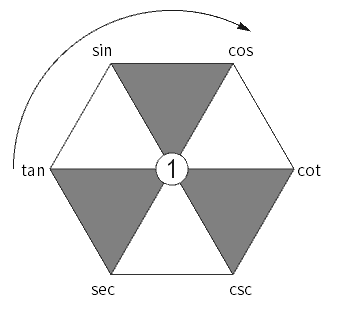
\includegraphics[width=0.4\textwidth]{img/triangle.png}
\end{figure}

% Geometric remarks
\begin{remark}
    \begin{itemize}
        \item On the gray triangle, the sum of the squares of the two numbers above is equal to the square of the number below,
            for instance, \(\tan^{2} x + 1 = \sec^{2}x\)
        \item The three trigonometric functions in the clockwise direction have the following properties: 
            $\tan x = \frac{\sin x}{\cos x}$, etc.
    \end{itemize}
\end{remark}

\section{Factorial Power}
\begin{definition}
    Rising factorials and falling factorials can be expressed in multiple notations.

    The Pochhammer symbol, introduced by Leo August Pochhammer, is one of the commonly used notations, 
    represented as \( x^{(n)} \) or \( (x)_n \).

    Ronald Graham, Donald Ervin Knuth, and Oren Patashnik introduced the symbols 
    \( x^{\bar{n}} \) and \( x^{\underline{n}} \) in their book \textit{Concrete Mathematics}.

    \paragraph{Definitions:}
    \begin{itemize}
        \item \textbf{Rising factorial:}
        \[
        x^{\bar{n}} = x(x+1)(x+2)\dots(x+n-1) = \frac{(x+n-1)!}{(x-1)!}.
        \]
        \item \textbf{Falling factorial:}
        \[
        x^{\underline{n}} = x(x-1)(x-2)\dots(x-n+1) = \frac{x!}{(x-n)!}.
        \]
    \end{itemize}

    \paragraph{Relationships:}
    \begin{itemize}
        \item Relationship between rising and falling factorials:
        \[
        x^{\bar{n}} = (x+n-1)^{\underline{n}}.
        \]
        \item Relationship with factorial:
        \[
        1^{\bar{n}} = n^{\underline{n}} = n!.
        \]
    \end{itemize}
\end{definition}

\section{Combination}
\begin{definition}{Combination}
    The number of ways to choose \(k\) elements from a set of \(n\) distinct elements, 
    denoted as \(\mathrm{C}_{n}^{k}\) or \(\binom{n}{k}\), is given by:
    \[
        \mathrm{C}_{n}^{k} = \binom{n}{k} = \frac{n!}{k!(n-k)!}.
    \]
\end{definition}

\begin{property}
    \begin{align*}
        &\mathrm{C}_{n}^{k} = \frac{\mathrm{A}_{n}^{k}}{k!} = \frac{n!}{(n-k)!k!} \\
        &\mathrm{C}_{n}^{k} = \mathrm{C}_{n}^{n-k} \\
        &\mathrm{C}_{n}^{k} = \mathrm{C}_{n-1}^{k-1} + \mathrm{C}_{n-1}^{k}
    \end{align*}
\end{property}

\begin{remark}
    The third property can be understood that to choose \(k\) elements from \(n+1\), 
    you can first take one element \(A\): 
    \begin{enumerate}
        \item  The number of ways that include \(A\) is \(\mathrm{C}_{n}^{k-1}\); 
        \item  The number of ways that do not include \(A\) is \(\mathrm{C}_{n}^{k}\).
    \end{enumerate}
\end{remark}


\chapter{Limits of Sequences and Continuity of Real Number System} 
\section{Convergent Sequences}
\begin{leftbarTitle}{Convergent Sequences}\end{leftbarTitle}

\begin{leftbarTitle}{Properties of Convergent Sequences}\end{leftbarTitle}



\begin{leftbarTitle}{Cauchy Proposition and Fitting Method}\end{leftbarTitle}
\begin{proposition}{Cauchy Proposition}\label{prop:Cauchy Proposition}
    Let \(\lim_{n \to \infty} x_n = l\), then:
    \[
        \lim_{n \to \infty} \frac{x_{1}+x_{2}+ \cdots +x_{n}}{n} = l.
    \]
\end{proposition}

\begin{note}
    \begin{enumerate}
        \item In the proposition, \(l\) can be \(+\infty\) or \(-\infty\).
        \item Let \(\lim_{n \to \infty} x_n = l\), then:
            \[
                \lim_{n \to \infty}\frac{x_{1}+x_{2}+ \cdots +x_{n}}{n}
                =\lim_{n \to \infty} \sqrt[n]{x_{1} x_{2} \cdots x_{n}} 
                =\lim_{n \to \infty} \frac{n}{\frac{1}{x_{1}} + \frac{1}{x_{2}} + \cdots + \frac{1}{x_{n}}}
                = l.
            \]
    \end{enumerate}
\end{note}

It can be proved directly by Stolz theorem~\ref{thm:Stolz Theorem}.
On top of that, it can also be proved by the \textbf{fitting method}.

\begin{proof}
    
\end{proof}

\begin{remark}
    To prove \(\lim_{n \to \infty} x_n = A\), 
    the key is to show that \(|x_n - A|\) can be arbitrarily small. 
    For this purpose, it is generally recommended to simplify the expression of \(x_n\) as much as possible. 
    However, in some cases, \(A\) can also be transformed into a form similar to \(x_n\). 
    This method is called the fitting method. 
    The core idea behind the method of fitting is to appropriately divide into units of \(1\) for analysis.
\end{remark}



\section{Indeterminate Form}
\begin{leftbarTitle}{Infinitely Large Quantities and Infinitesimal Quantities}\end{leftbarTitle}

\begin{leftbarTitle}{Indeterminate Forms}\end{leftbarTitle}

\begin{theorem}{Stolz-Cesàro theorem}\label{thm:Stolz Theorem}
    \begin{description}
        \item[Type \(\frac{0}{0}\)] Let \(\{a_n\}, \{b_n\}\) be two infinitesimal sequences, 
            where \(\{a_n\}\) is also a strictly monotonic decreasing sequence. If  
            \[
            \lim_{n \to \infty} \frac{b_{n+1} - b_n}{a_{n+1} - a_n} = l \, (\text{finite or } \pm\infty),
            \]  
            then  
            \[
            \lim_{n \to \infty} \frac{a_n}{b_n} = l.
            \] 
        \item[Type \(\frac{\text{*}}{\infty}\)] Let \(\{a_n\}\) be a strictly monotonic increasing sequence 
            of divergent large quantities. If  
            \[
            \lim_{n \to \infty} \frac{b_{n+1} - b_n}{a_{n+1} - a_n} = l \, (\text{finite or } \pm\infty),
            \]  
            then  
            \[
            \lim_{n \to \infty} \frac{a_n}{b_n} = l.
            \]
    \end{description}
\end{theorem}
\begin{note}
    \begin{enumerate}
        \item The inverse proposition of Stolz's Theorem does not hold.
        \item If \(a_1\) is an undefined infinite quantity \(\infty\), Stolz Theorem does not hold.
    \end{enumerate}
\end{note}

\begin{theorem}{Silverman-Toeplitz Theorem}\label{thm:Toeplitz Theorem}
    Let
    \[
        \begin{bmatrix}
        y_1 \\ y_2 \\ \vdots \\ y_n \\ \vdots
        \end{bmatrix}
        =
        \begin{bmatrix}
        a_{11} & 0 & \cdots & 0 \\
        a_{21} & a_{22} & \cdots & 0 \\
        \vdots & \vdots & \ddots & \vdots \\
        a_{n1} & a_{n2} & \cdots & a_{nn} \\
        \vdots & \vdots &        & \vdots \\
        \end{bmatrix}
        \begin{bmatrix}
        x_1 \\  x_2 \\  \vdots \\   x_n \\ \vdots
        \end{bmatrix},
    \]
    where the infinite triangular matrix satisfies:
    \begin{enumerate}
        \item \(\forall j, \lim_{n \to \infty} a_{nj} = 0.\)(Every column sequence converges to \(0\).)
        \item \(\sup_{i\in \mathbb{N}} \sum_{j=1}^{i} \left| a_{ij} \right| < \infty.\)(The absolute row sums are bounded.)
    \end{enumerate}
    And \(\lim_{n \to \infty} x_n = l\).
    We denote \(y_{n}\) as the weighted sum sequence: \(y_{n} = \sum_{j=1}^n a_{nj} x_j\).
    Then the following results hold:
    \begin{enumerate}
        \item If \(l=0\), then  \(\lim_{n \to \infty} y_n = 0\).
        \item If \(l \neq 0\) and \(\lim_{n \to \infty}\sum_{j=1}^{n} a_{ij}=1 \), then \(\lim_{n \to \infty} y_n = l\).
    \end{enumerate}
\end{theorem}




\section{Subsequences}
\begin{leftbarTitle}{Subsequences}\end{leftbarTitle}

\begin{leftbarTitle}{Upper Limits and Lower Limits}\end{leftbarTitle}


\section{Completeness of The Real Numbers}
\begin{leftbarTitle}{Dedkind Completeness}\end{leftbarTitle}

\begin{leftbarTitle}{Least Upper Bound Property}\end{leftbarTitle}

\begin{leftbarTitle}{Monotone Convergence Theorem}\end{leftbarTitle}

\begin{leftbarTitle}{Bolzano-Weierstrass Theorem}\end{leftbarTitle}

\begin{leftbarTitle}{Nested Interval Theorem}\end{leftbarTitle}

\begin{leftbarTitle}{Cauchy Completeness}\end{leftbarTitle}
\begin{definition}{Cauchy Sequence}
    A sequence \(\{x_n\}\) is called a \textbf{Cauchy sequence} if for any \(\varepsilon > 0\), 
    there exists a positive integer \(N\) such that when \(m,n > N\), 
    \[
        \left|x_n - x_m\right| < \varepsilon.
    \]
\end{definition}

\begin{theorem}{Cauchy Convergence Criterion for Sequences}\label{thm:Cauchy Convergence Criterion for Sequences}
    A sequence \(\{x_n\}\) converges if and only if it is a Cauchy sequence.
\end{theorem}


\begin{leftbarTitle}{Heine-Borel Theorem}\end{leftbarTitle}

\section{Iterative Sequences}
Formally, \(x_{0}\) is a \textbf{fixed point} of the function \(f\) if \(f(x_{0}) = x_{0}\).

\begin{theorem}{Banach Fixed-Point Theorem (Contraction Mapping Theorem)}\label{thm:Banach Fixed-Point Theorem}
    There exists a contraction mapping (in~\ref{def:Lipschitz Continuity}) \(f\) on an interval \(I\),
    which admits a unique fixed point \(x^{*}\in I\).
    Furthermore, \(x^{*}\) can be found as follows:
    start with an arbitrary point \(x_{0}\in I\) and define the iterative sequence
    \(x_{n+1}=f(x_n)\) for \(n=0,1,2,\cdots\).
    Then \(\lim_{n \to \infty} x_n = x^{*}\).
\end{theorem}

\begin{remark}
    The following inequalities are equivalent and describe the speed of convergence:  
    \begin{gather*}
        \left| x_{n} - x^{*} \right|  \leqslant \frac{L^{n}}{1-L} \left| x_{1} - x_{0} \right|, \\
        \left| x_{n+1} - x^{*} \right| \leqslant \frac{L}{1-L} \left| x_{n+1} - x_{n} \right|, \\
        \left| x_{n+1} - x^{*} \right| \leqslant L \left| x_{n} - x^{*} \right|.
    \end{gather*}
    Any such value of \(L<1\) is the Lipschitz constant for \(f\), 
    and the smallest one is sometimes called \textbf{the best Lipschitz constant} of \(L\).
\end{remark}



\chapter{Limits and Continuity of Functions}
\section{Limits of Functions}
\begin{leftbarTitle}{Definition of Limit}\end{leftbarTitle}

\begin{leftbarTitle}{Limits of Functions and Sequences}\end{leftbarTitle}
\begin{theorem}{Heine Theorem}\label{thm:Heine Theorem}
    Let \(f\) be a function defined on a deleted neighborhood \(\mathring{U}(x_{0})\) of \(x_{0}\).
    The following two statements are equivalent:
    \begin{enumerate}
        \item \(\lim_{x \to x_{0}} f(x) = A\).
        \item For any sequence \(\{x_n\}\subset \mathring{U}(x_{0})\) with \(\lim_{n \to \infty} x_n = x_0\),
            we have \(\lim_{n \to \infty} f(x_n) = A\) for the sequence \(\{f(x_n)\}\).
    \end{enumerate}
\end{theorem}

\section{Continuous Functions}

\section{Infinitesimal and Infinite Quantities}

\section{Continuous Functions on Closed Intervals}
\begin{leftbarTitle}{Concerning Theorems}\end{leftbarTitle}


\begin{theorem}{The Bolzano-Cauchy Intermediate-Value Theorem}\label{thm:Indeterminate Value Theorem}

\end{theorem}

\begin{theorem}{Zero Point Existence Theorem}\label{thm:Zero Point Existence Theorem}

\end{theorem}

\begin{leftbarTitle}{Uniform Continuity and Lipschitz Continuity}\end{leftbarTitle}

\begin{definition}{Uniform Continuity}
    
\end{definition}

\begin{theorem}{Uniform Continuity Theorem}
    
\end{theorem}


\begin{theorem}{Cantor's Theorem}
    
\end{theorem}


\begin{definition}{Lipschitz Continuity}\label{def:Lipschitz Continuity}
    If there exists a constant \(L > 0\) such that for any \(x_1, x_2 \in I\), 
    \[
        \left| f(x_{1}) - f(x_{2}) \right| \leqslant L \left| x_{1} - x_{2} \right|,
    \]
    then \(f\) is called \textbf{Lipschitz continuous} on \(I\).

    Specially, if \(L < 1\), then \(f\) is called a \textbf{contraction mapping} on \(I\).
\end{definition}

\begin{remark}
    \begin{itemize}
        \item If \(f\) is Lipschitz continuous on \(I\), then \(f\) is uniformly continuous on \(I\).
            (\(\forall \varepsilon > 0\), just let \(\delta = \frac{\varepsilon}{L}\))
        \item If \(f\) is uniformly continuous on \(I\), then \(f\) is continuous on \(I\).
        \item The converse of the above two statements does not hold.
    \end{itemize}
\end{remark}




\section{Period Three Implies Chaos}



\section{Functional Equations}

\chapter{Differential}
\section{Differential and Derivative}

\begin{leftbarTitle}{Basic Differential Rules and Formulas}\end{leftbarTitle}
\[
\begin{array}{|c|c|c|}
\hline
 & \textbf{Derivative Rules} & \textbf{Differential Rules} \\
\hline
\text{Linear Combination} & (c_{1}f+c_{2}g)' = c_{1}f' + c_{2}g' & 
    \mathrm{d}(c_{1}f+c_{2}g) = c_{1}\mathrm{d}f + c_{2}\mathrm{d}g \\
\hline
\text{Product Rule} & (fg)' = f'g + fg' & \mathrm{d}(fg) = g\mathrm{d}f + f\mathrm{d}g \\
\hline
\text{Quotient Rule} & \left( \frac{f}{g} \right)' = \frac{f'g - fg'}{g^2} & 
    \mathrm{d}\left( \frac{f}{g} \right) = \frac{g\mathrm{d}f - f\mathrm{d}g}{g^2} \\
\hline
\text{Inverse Function} & [f^{-1}(y)]' = \frac{1}{f'(x)} & \mathrm{d}x = \frac{\mathrm{d}y}{f'(x)} = [f^{-1}(y)]'\mathrm{d}y \\
\hline
\text{Chain Rule} & [f(g(x))]' = f'(u)g'(x) & \mathrm{d}[f(g(x))] = f'(u)g'(x)\mathrm{d}x \\
\hline
\end{array}
\]



\[
\begin{array}{|c|c|}
\hline
\textbf{Derivative} & \textbf{Differential} \\
\hline
(C)'=0 & \mathrm{d}(C)=0\cdot \mathrm{d}x=0 \\
\hline
(x^\alpha)'=\alpha x^{\alpha-1} & \mathrm{d}(x^\alpha)=\alpha x^{\alpha-1}\mathrm{d}x \\ \hline
\rowcolor{gray!30} & \\ \hline
(\sin x)'=\cos x & \mathrm{d}(\sin x)=\cos x\mathrm{d}x \\
\hline
(\cos x)'=-\sin x & \mathrm{d}(\cos x)=-\sin x\mathrm{d}x \\
\hline
(\tan x)'=\sec^2x & \mathrm{d}(\tan x)=\sec^2x\mathrm{d}x \\
\hline
(\cot x)'=-\csc^2x & \mathrm{d}(\cot x)=-\csc^2x\mathrm{d}x \\
\hline
(\sec x)'=\tan x\sec x & \mathrm{d}(\sec x)=\tan x\sec x\mathrm{d}x \\
\hline
(\csc x)'=-\cot x\csc x & \mathrm{d}(\csc x)=-\cot x\csc x\mathrm{d}x \\
\hline
(\arcsin x)'=\frac{1}{\sqrt{1-x^2}} & \mathrm{d}(\arcsin x)=\frac{1}{\sqrt{1-x^2}}\mathrm{d}x \\
\hline
(\arccos x)'=-\frac{1}{\sqrt{1-x^2}} & \mathrm{d}(\arccos x)=-\frac{1}{\sqrt{1-x^2}}\mathrm{d}x \\
\hline
(\arctan x)'=\frac{1}{1+x^2} & \mathrm{d}(\arctan x)=\frac{1}{1+x^2}\mathrm{d}x \\
\hline
(\mathrm{arccot} x)'=-\frac{1}{1+x^2} & \mathrm{d}(\mathrm{arccot} x)=-\frac{1}{1+x^2}\mathrm{d}x \\
\hline
\hline
(a^x)'=\ln a\cdot a^x, \, (e^x)'=e^x & \mathrm{d}(a^x)=\ln a\cdot a^x\mathrm{d}x, \, \mathrm{d}(e^x)=e^x\mathrm{d}x \\
\hline
(\log_{a}x)'=\frac{1}{x\ln a}, \, (\ln x)'=\frac{1}{x} & \mathrm{d}(\log_{a}x)=\frac{1}{x\ln a}\mathrm{d}x, \, \mathrm{d}(\ln x)=\frac{1}{x}\mathrm{d}x \\ \hline
\rowcolor{gray!30} & \\ \hline
(\mathrm{sh}\,x)'=\mathrm{ch}\,x & \mathrm{d}(\mathrm{sh}\,x)=\mathrm{ch}\,x\mathrm{d}x \\
\hline
(\mathrm{ch}\,x)'=\mathrm{sh}\,x & \mathrm{d}(\mathrm{ch}\,x)=\mathrm{sh}\,x\mathrm{d}x \\
\hline
(\mathrm{th}\,x)'=\mathrm{sech}^2\,x & \mathrm{d}(\mathrm{th}\,x)=\mathrm{sech}^2\,x\mathrm{d}x \\
\hline
(\mathrm{cth}\,x)'=-\mathrm{csch}^2\,x & \mathrm{d}(\mathrm{cth}\,x)=-\mathrm{csch}^2\,x\mathrm{d}x \\
\hline
(\mathrm{arcsh}\,x)'=\frac{1}{\sqrt{1+x^2}} & \mathrm{d}(\mathrm{arcsh}\,x)=\frac{1}{\sqrt{1+x^2}}\mathrm{d}x \\
\hline
(\mathrm{arcch}\,x)'=\frac{1}{\sqrt{x^2-1}} & \mathrm{d}(\mathrm{arcch}\,x)=\frac{1}{\sqrt{x^2-1}}\mathrm{d}x \\
\hline
(\mathrm{arcth}\,x)'=(\mathrm{arccth}\,x)'=\frac{1}{1-x^2} & 
    \mathrm{d}(\mathrm{arcth}\,x)=\mathrm{d}(\mathrm{arccth}\,x)=\frac{1}{1-x^2}\mathrm{d}x \\ \hline
\rowcolor{gray!30} & \\ \hline
\ln(x+\sqrt{x^2+a^2})'=\frac{1}{\sqrt{x^2+a^2}} & \mathrm{d}[\ln(x+\sqrt{x^2+a^2})]=\frac{\mathrm{d}x}{\sqrt{x^2+a^2}} \\
\hline
\end{array}
\]

\section{Higher-Order Derivatives}

Some useful formulas of higher-order derivatives:
\begin{gather*}
    (a^{x})^{(n)} = (\ln a)^n a^x,\\
    (\sin \alpha x)^{(n)} = \alpha^n \sin\left(\alpha x + \frac{n\pi}{2}\right), \\
    (\cos \alpha x)^{(n)} = \alpha^n \cos\left(\alpha x + \frac{n\pi}{2}\right),\\
    (\ln x)^{(n)} = \frac{(-1)^{n-1}(n-1)!}{x^n}, \\ 
    (x^\alpha)^{(n)} = \alpha(\alpha-1)\cdots(\alpha-n+1)x^{\alpha-n}.
\end{gather*}

In order to obtain the higher-order derivative of two or more functions' linear combination and product,
we need to use the following theorems.

\begin{theorem}{Linear Operation of Higher-Order Derivatives}
    If \(f,g\in D^{(n)}(I)\), then for any constants \(c_{1}, c_{2}\in \mathbb{R}\),
    \[
        (c_{1}f + c_{2}g)^{(n)} = c_{1}f^{(n)} + c_{2}g^{(n)}.
    \]
\end{theorem}

\begin{theorem}{Leibniz's Formula}
    If \(f,g\in D^{(n)}(I)\), then
    \[
        (fg)^{(n)} = \sum_{k=0}^{n} \binom{n}{k} f^{(k)} g^{(n-k)}.
    \]
\end{theorem}

\begin{caution}
    Note the distinction: 
    \begin{itemize}
        \item \(\mathrm{d}x^2\) represents the square of the differential of the independent variable, i.e., \((\mathrm{d}x)^2\);
        \item \(\mathrm{d}^2x\) represents the second differential of the independent variable, \(\mathrm{d}(\mathrm{d}x)\);
        \item \(\mathrm{d}(x^2)\) represents the differential of \(x^2\), which is \(2x\mathrm{d}x\).
    \end{itemize}
\end{caution}

\section{Differential Mean Value Theorems}
\begin{definition}{Argmax and Argmin}
    Let \(f(x)\) is defined on \((a,b)\), \(x_{0}\in (a,b)\).
    If there exists \(U(x_{0}, \delta)\subset (a,b)\) such that \(f(x)\leqslant f(x_{0})\) on it,
    then \(x_{0}\) is called a arguments of the maxima point of \(f\),
    and \(f(x_{0})\) is referred to as the corresponding arguments of the maxima (abbreviated arg max or argmax).

    The definition of the argmin is analogous.
\end{definition}


\begin{lemma}{Fermat's Lemma}
    If \(f\) is differentiable at \(x_{0}\) which is a local extremum, then \(f'(x_{0}) = 0\).
\end{lemma}

\begin{theorem}{Rolle's Theorem}
    If \(f\in C[a,b], f\in D(a,b)\) and \(f(a) = f(b)\), then there exists \(\xi\in (a,b)\) such that \(f'(\xi) = 0\).

    \underline{\textbf{Enhanced Version:}}If \(f\in D(a,b)\)(finite or infinite interval), 
    and \(\lim_{x \to a^{+}} f(x) = \lim_{x \to b^{-}} f(x) \) , 
    then there exists \(\xi\in (a,b)\) such that \(f'(\xi) = 0\).
\end{theorem}

\begin{theorem}{Lagrange's Mean Value Theorem}
    If \(f\in C[a,b], f\in D(a,b)\), then there exists \(\xi\in (a,b)\) such that
    \[
        f'(\xi) = \frac{f(b) - f(a)}{b - a}.
    \]
\end{theorem}

\begin{theorem}{Cauchy's Mean Value Theorem}
    If \(f,g\in C[a,b], f,g\in D(a,b)\) and \(g'(x) \neq 0\) for all \(x\in (a,b)\), 
    then there exists \(\xi\in (a,b)\) such that
    \[
        \frac{f'(\xi)}{g'(\xi)} = \frac{f(b) - f(a)}{g(b) - g(a)}.
    \]
\end{theorem}


\vspace{0.7cm}
\begin{note}
The following types of problems commonly appear in proofs related to intermediate values in differential calculus:
\begin{enumerate}
    \item Prove the existence of a point \(\xi\) such that \(F(\xi, f(\xi), f'(\xi)) = 0\).
        Problems of this type generally involve constructing auxiliary functions and applying Rolle's theorem. 
        The commonly used auxiliary functions include:
        \[
        \begin{aligned}
        \xi f'(\xi) + f(\xi) &= 0, \quad x f(x), \\
        \xi f'(\xi) + nf(\xi) &= 0, \quad x^n f(x), \\
        \xi f'(\xi) - f(\xi) &= 0, \quad e^x f(x), \\
        f'(\xi) + \lambda f(\xi) &= 0, \quad e^{-x} f(x), \\
        f'(\xi) + f(\xi) &= 0, \quad x^n f(x), \\
        f'(\xi) - f(\xi) &= 0, \quad x f(x). \\
        \end{aligned}
        \]
    
    \item Prove the existence of two points \(\xi, \eta\) (i.e., two intermediate values) 
        such that \(F(\xi, f(\xi), f'(\xi), \eta, f(\eta), f'(\eta)) = 0\).
        These problems can be divided into the following categories:
        \begin{description}
            \item [\(\xi \neq \eta\)] Problems of this type usually occur in the same interval \([a, b]\) and 
                employ theorems of \underline{double} differentiation intermediate values 
                such as the Lagrange mean value theorem or Cauchy's mean value theorem. 
                The specific choice of auxiliary functions often includes terms like \(\xi\) and 
                other variables determined after \underline{decomposition}.
            \item [\(\xi = \eta\)] Such problems cannot occur within the same interval \([a, b]\). 
                They use double differentiation mean value theorems by \underline{splitting} \([a, b]\) into 
                two intervals \([a,c]\) and \([c,b]\), 
                applying the Lagrange mean value theorem separately to each interval. 
                Here, the \underline{selection} of \(\xi\) and \(\eta\) is key.
        \end{description}

    \item As a rule, when conditions in a theorem involve additional constraints about \underline{higher-order} derivatives, 
        it is necessary to use Taylor's intermediate value theorem.
\end{enumerate}
\end{note}



\section{Theorems about Derivatives}

\begin{theorem}{Darboux's Intermediate Value Theorem for Derivatives}
    If \(f(x)\in D[a,b]\), and \(f'_{+}(a)\cdot f'_{-}(b)<0\),
    then there at least exists \(\xi\in (a,b)\) such that \(f'(\xi) = 0\).
\end{theorem}

\begin{theorem}{Theorem on the Limit of Derivatives}
    If \(f(x)\in C(U(x_{0})),\mathring{D}(U(x_{0}))\), and \(\lim_{x \to x_{0}} f'(x) = A\),
    then \(f\) is differentiable at \(x_{0}\) and \(f'(x_{0}) = A\).
\end{theorem}
\begin{remark}
    In fact, \(\lim_{x \to x_{0}} f'(x) = A\) has already been shown to imply that \(f\in \mathring{D}(U(x_{0}))\).
\end{remark}

\section{Taylor Theorem}
\begin{leftbarTitle}{L'Hôpital's Rule}\end{leftbarTitle}

\begin{leftbarTitle}{Taylor Formula}\end{leftbarTitle}


\begin{leftbarTitle}{Maclaurin Formula}\end{leftbarTitle}
\begin{lemma}
    If \(f(x)\) has \(n+2\) derivatives in some neighborhood of \(x_{0}\), 
    then the derivative of its \(n+1\)th degree Taylor polynomial 
    is exactly the \(n\)th degree Taylor polynomial of \(f'(x)\).
\end{lemma}

Taylor formula at \(x_{0} = 0\) is called the \textbf{Maclaurin formula}.
Some common Maclaurin formulas are as follows:
\begin{gather*}
    e^{x} = 1 + \frac{x}{1!} + \frac{x^2}{2!} + \frac{x^3}{3!} + \cdots + \frac{x^n}{n!} + o(x^n), \\
    \ln(1+x) = x - \frac{x^2}{2} + \frac{x^3}{3} - \cdots + (-1)^{n-1}\frac{x^n}{n} + o(x^n), \\
\end{gather*}
\begin{gather*}
    \sin x = x - \frac{x^3}{3!} + \frac{x^5}{5!} - \cdots + (-1)^{n-1}\frac{x^{2n-1}}{(2n-1)!} + o(x^{2n}), \\
    \cos x = 1 - \frac{x^2}{2!} + \frac{x^4}{4!} - \cdots + (-1)^{n}\frac{x^{2n}}{(2n)!} + o(x^{2n+1}), \\
\end{gather*}
\begin{gather*}
    \arctan x = x - \frac{x^3}{3} + \frac{x^5}{5} - \cdots + (-1)^{n-1}\frac{x^{2n-1}}{2n-1} + o(x^{2n}), \\
    \arcsin x = x + \frac{1}{2}\frac{x^3}{3} + \frac{1\cdot 3}{2\cdot 4}\frac{x^5}{5} + \cdots + 
        \frac{(2n-1)!!}{(2n)!!}\frac{x^{2n+1}}{2n+1} + o(x^{2n+2}). \\
\end{gather*}
Specially, 
\[
(1+x)^{\alpha} = \sum_{k=0}^{\alpha} \binom{\alpha}{k} x^k + o(x^{n}),
\]
\begin{itemize}
    \item if \(\alpha = n\in \mathbb{N}^{+}\), that is Newton's binomial formula 
        \((1+x)^n = 1 + \binom{n}{1}x + \binom{n}{2}x^2 + \cdots + \binom{n}{n}x^n\); 
    \item if \(\alpha = \frac{1}{2}\), then
        \((1+x)^{\frac{1}{2}} = 1 + \frac{1}{2}x - \frac{1}{8}x^2 + \cdots\);
    \item if \(\alpha = -1\), then
        \((1+x)^{-1} = 1 - x + x^2 - x^3 + \cdots\);
    \item if \(\alpha = -\frac{1}{2}\), then
        \((1+x)^{-\frac{1}{2}} = 1 - \frac{1}{2}x + \frac{3}{8}x^2 - \cdots\).
\end{itemize}

\begin{leftbarTitle}{Euler and Bernoulli Numbers}\end{leftbarTitle}
\begin{definition}{Euler Numbers}
    The Euler numbers \(E_n\) are defined by the Taylor series expansion of the secant function:
    \[
        \operatorname{sech} x = \frac{2}{e^x + e^{-x}} = \sum_{n=0}^{\infty} E_n \frac{x^n}{n!}.
    \]
    The odd-indexed Euler numbers are all zero. 
    The even-indexed ones have alternating signs. Some values are:
    \[
        E_0 = 1, \quad E_2 = -1, \quad E_4 = 5, \quad E_6 = -61, \quad E_8 = 1385.
    \]
\end{definition}

\begin{definition}{Bernoulli Numbers}
    The Bernoulli numbers \(B_n\) are defined by the Taylor series expansion of the function \(\frac{x}{e^x - 1}\):
    \[
        \frac{x}{e^x - 1} = \sum_{n=0}^{\infty} B_n \frac{x^n}{n!}.
    \]
    Some values are:
    \[
        B_0 = 1, \quad B_2 = \frac{1}{6}, \quad B_4 = -\frac{1}{30}, \quad B_6 = \frac{1}{42}, \quad B_8 = -\frac{1}{30}.
    \]
    Notably, all odd-indexed Bernoulli numbers (except \(B_1 = -\frac{1}{2}\)) are zero.
\end{definition}

\begin{remark}
    Euler and Bernoulli numbers are widely used in number theory, combinatorics, and numerical analysis.
    For example, in the infinite series:
    \[
    \sum_{n=1}^{\infty}  \frac{1}{n^{2k}} = (-1)^{k-1} \frac{(2\pi)^{2k}}{2(2k)!} B_{2k},\quad k \in \mathbb{N}^{+},
    \]
    when \(k=1\), it gives the famous Basel problem result:
    \[
    \sum_{n=1}^{\infty}  \frac{1}{n^{2}} = \frac{\pi^2}{6}.
    \]
\end{remark}

With the help of Bernoulli numbers, we have
\[
\tan x = \sum_{n=0}^{\infty} \frac{B_{2n}}{2n} \frac{x^{2n}}{(2n)!} = 
x + \frac{x^3}{3} + \frac{2}{15}x^5 + \cdots.
\]


\section{Properties of Functions}
\begin{leftbarTitle}{Monotonicity and Convexity}\end{leftbarTitle}
\begin{definition}{Convex Function}
    A function \(f\) is called \textbf{convex} on an interval \(I\) if for any \(x_1, x_2 \in I\) and 
    \(t \in [0,1]\), the following inequality holds:
    \[
        f(t x_1 + (1-t)x_2) \leqslant t f(x_1) + (1-t)f(x_2).
    \]
    If the inequality is strict for \(x_1 \neq x_2\) and \(t \in (0,1)\), 
    then \(f\) is called \textbf{strictly convex} on \(I\).

    Conversely, if the inequality is reversed, then \(f\) is called \textbf{concave} or \textbf{concave down} on \(I\).
\end{definition}
\begin{figure}[h]
    \centering
    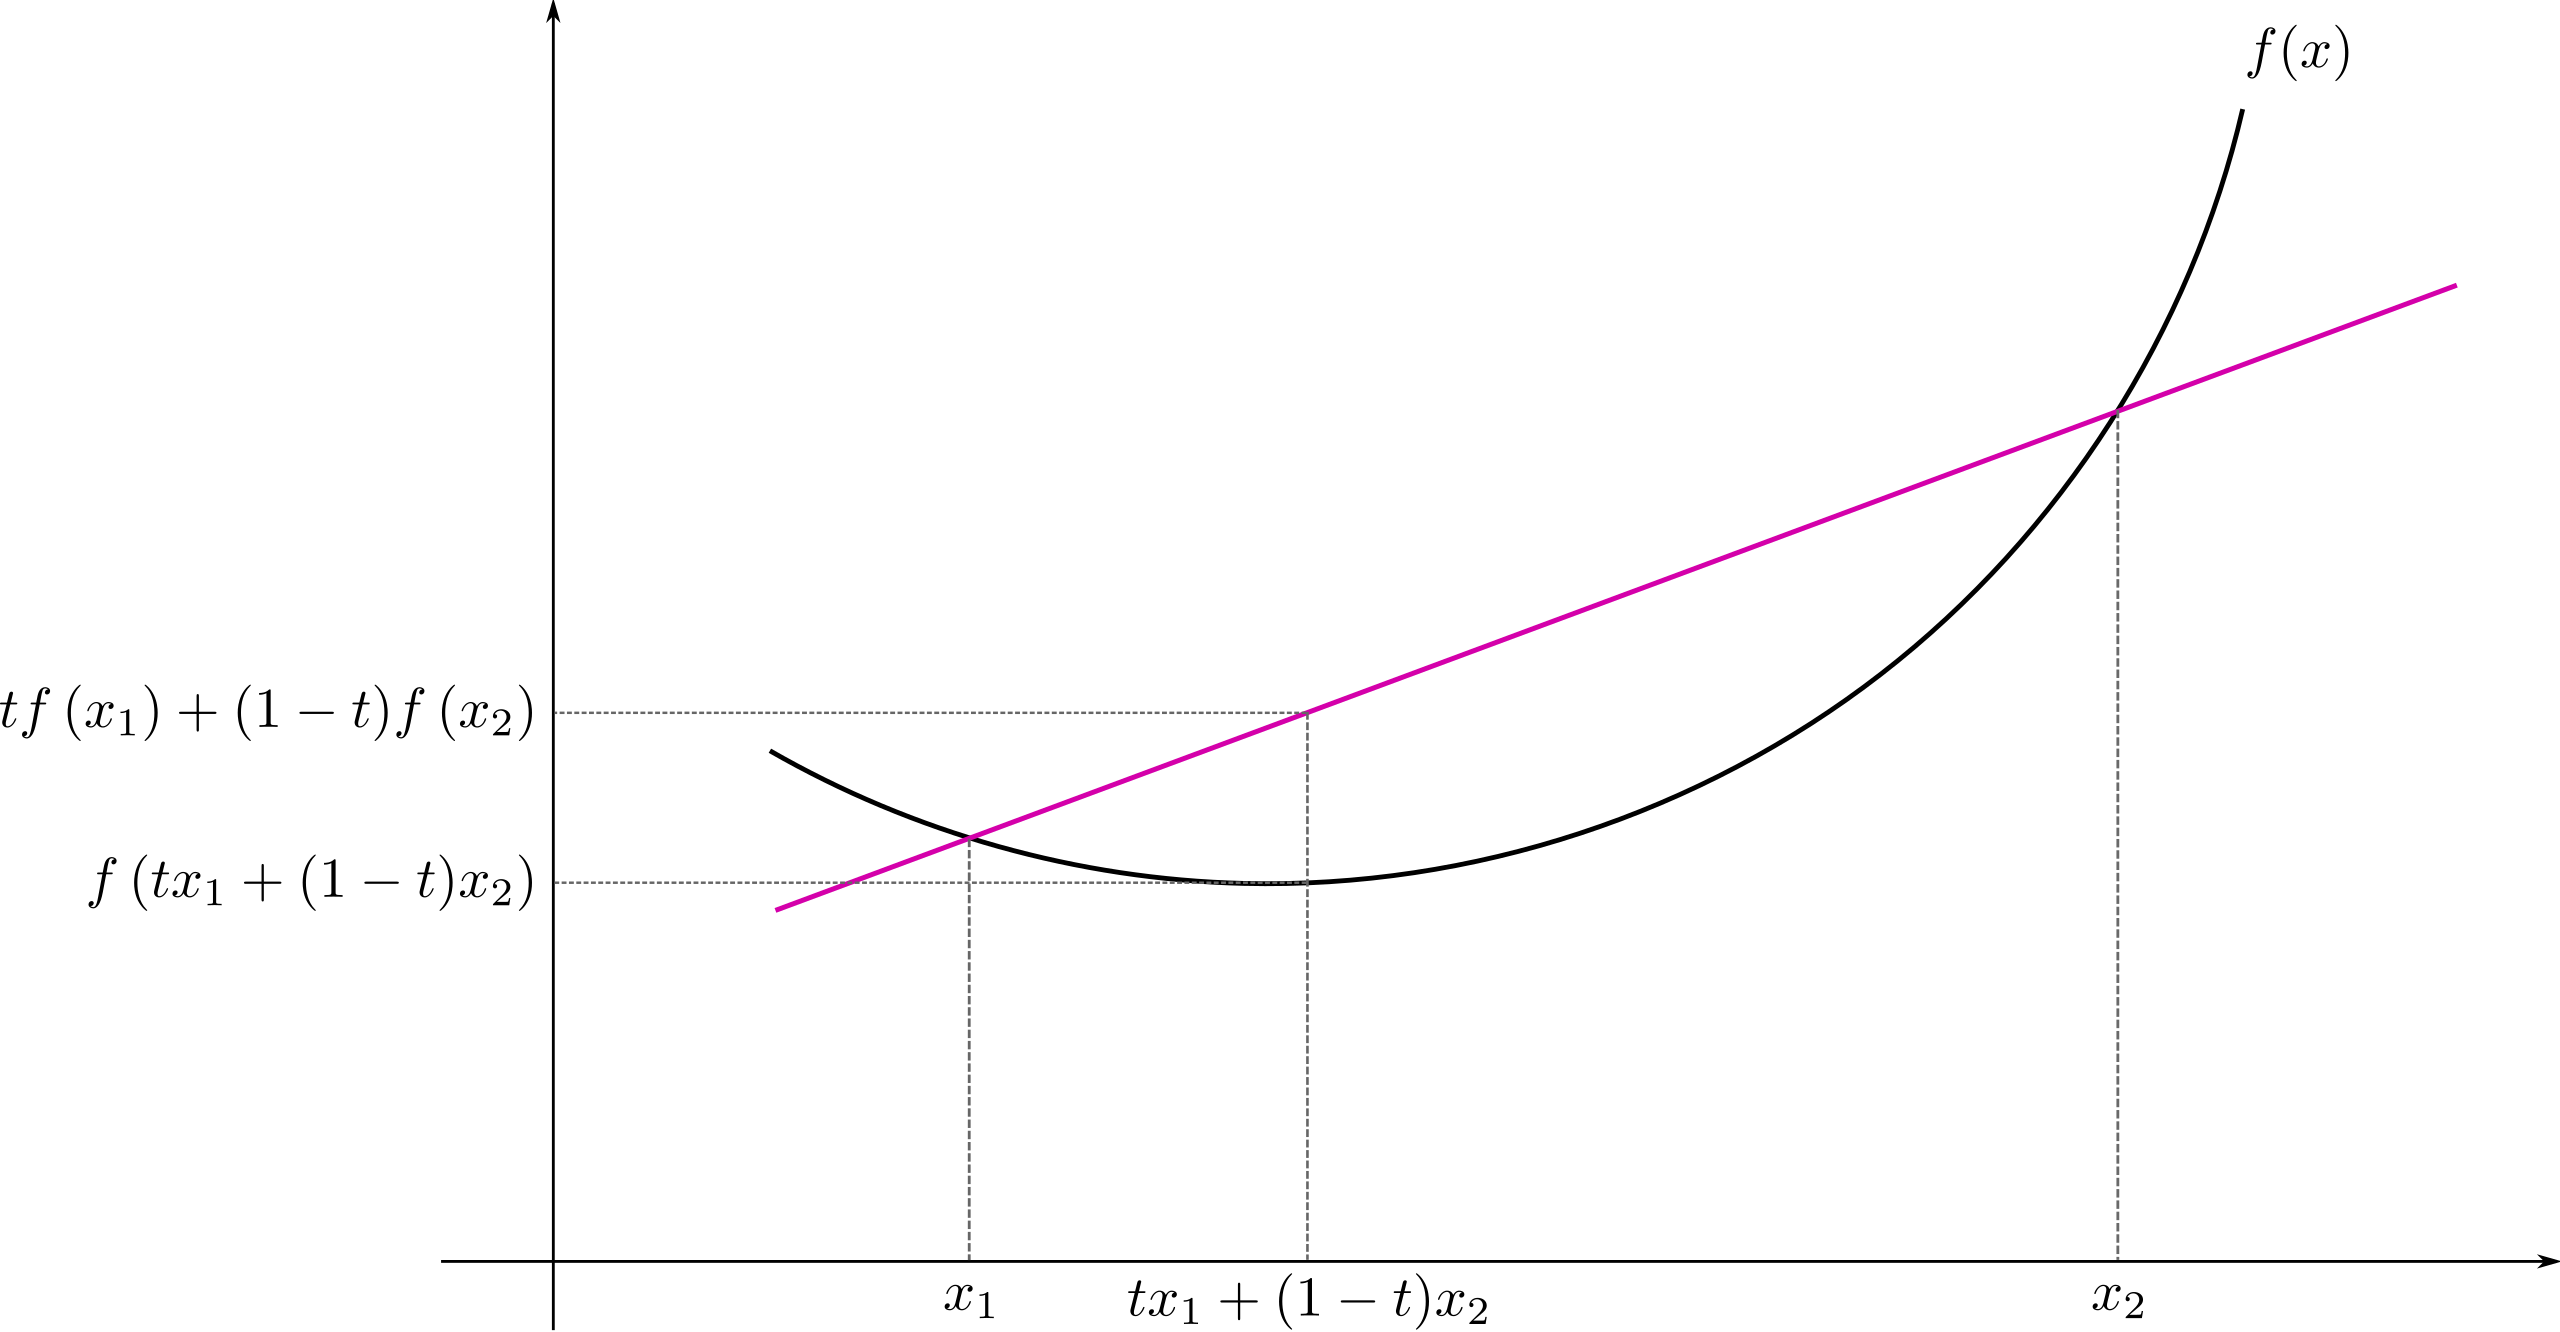
\includegraphics[width=0.8\textwidth]{img/ConvexFunction.png}
\end{figure}

\begin{theorem}
    Mark above definition as Definition 1, give the following statements:
    \begin{enumerate}
        \setcounter{enumi}{1} % 设置计数器,从 2 开始
        \item (\textbf{Jensen Definition}) A function \(f\) is called convex on an interval \(I\) 
            if for any \(x_1, x_2 \in I\):
            \[
                f\left( \frac{x_1 + x_2}{2} \right) \leqslant \frac{f(x_1) + f(x_2)}{2}.
            \]
        \item A function \(f\) is called convex on an interval \(I\) 
            if for any \(x_1, x_2, \cdots, x_n \in I\):
            \[
                f\left( \frac{x_1 + x_2 + \cdots + x_n}{n} \right) \leqslant \frac{f(x_1) + f(x_2) + \cdots + f(x_n)}{n}.
            \]
        \item A function \(f\) is called convex on an interval \(I\) 
            if the tangent line at any point lies below the graph of the function.
    \end{enumerate}
    Then,
    \begin{itemize}
        \item Definitions 2 and 3 are equivalent. 
        \item When \(f\) is continuous, Definition 1, 2, 3 is equivalent.
        \item When \(f\) is differentiable, all four definitions are equivalent.
    \end{itemize}
\end{theorem}


\begin{theorem}{Jensen Inequality}
    If \(f\) is convex on an interval \(I\), 
    then for any \(x_1, x_2, \cdots, x_n \in I\) and any \(t_1, t_2, \cdots, t_n > 0\) 
    such that \(t_1 + t_2 + \cdots + t_n = 1\),
    the following inequality holds:
    \[
        f(t_1 x_1 + t_2 x_2 + \cdots + t_n x_n) \leqslant t_1 f(x_1) + t_2 f(x_2) + \cdots + t_n f(x_n).
    \]

    Specially, when \(t_1 = t_2 = \cdots = t_n = \frac{1}{n}\), it reduces to Definition 3.
\end{theorem}


Next, we present derivative-based criteria for monotonicity and convexity:
\begin{theorem}
    \begin{enumerate}
        \item If \(f \in D(I)\), then \(f\) is increasing (decreasing) on \(I\) 
            if and only if \(f'(x) \geq 0\) (\(f'(x) \leqslant 0\)) for all \(x \in I\). 
        \item If \(f \in D^{(2)}(I)\), then \(f\) is convex (concave) on \(I\) 
            if and only if \(f''(x) \geq 0\) (\(f''(x) \leqslant 0\)) for all \(x \in I\).
    \end{enumerate}
\end{theorem}

\begin{note}
    If \(f'(x) > 0\) (\(f''(x) > 0\)) for all \(x \in I\), then \(f\) is strictly increasing (convex) on \(I\).
    Even though the condition weakens to holding except at finitely many points,
    the conclusion of strict monotonicity (convexity) still holds.
    For example, \(f(x) = x^3\) is strictly increasing on \(\mathbb{R}\)
    despite \(f'(0) = 0\).
\end{note}


\begin{leftbarTitle}{Argmax and Argmin}\end{leftbarTitle}


\begin{leftbarTitle}{Asymptote}\end{leftbarTitle}







\section{Applications}




\chapter{Indefinite Integral}

\section{Two Common Integration Methods}
\begin{leftbarTitle}{Integration Methods}\end{leftbarTitle}
\begin{definition}{Integration by Parts}
    Let \( u(x) \) and \( v(x) \) be two differentiable functions,
    and at least one of them has an antiderivative.
    Then the integration by parts formula states that:
    \[
        \int u \, \mathrm{d}v = uv - \int v \, \mathrm{d}u.
    \]
\end{definition}

\begin{definition}{Substitution Method}
\end{definition}

Some common substitutions are as follows:
\begin{description}
    \item[Trigonometric Substitution] When restoring variables, auxiliary right triangles is often utilized.
        \begin{description}
            \item[Sine] \( \sqrt{a^2 - x^2} \): \( x = a \sin t \) or \( x = a \cos t \)
            \item[Tangent] \( \sqrt{a^2 + x^2} \): \( x = a \tan t \) or \( x = a \sinh t \)
            \item[Secant] \( \sqrt{x^2 - a^2} \): \( x = a \sec t \) or \( x = a \cosh t \)
        \end{description}
    \item[Irreational Substitution] 
        \begin{itemize}
            \item If the integrand contains \( \sqrt[n]{x} \),
                one can use the substitution \( t = \sqrt[n]{x} \) to simplify the expression.
            \item If the integrand contains \( \sqrt[n]{\frac{\alpha x + \beta}{\gamma x + \delta}} \),
                one can use the substitution \( t = \sqrt[n]{\frac{\alpha x + \beta}{\gamma x + \delta}} \) to simplify the expression.
        \end{itemize}
    \item[Reciprocal Substitution] If the degree of the numerator is lower than that of the denominator according to \(x\) 
        one can use the substitution \( x = \frac{1}{t} \) to reduce the degree.
\end{description}

\begin{leftbarTitle}{Basic Integration Formulas}\end{leftbarTitle}
\[
\begin{array}{|c|c|}
\hline
\textbf{Integral} & \textbf{Result} \\
\hline
\int a \, \mathrm{d}x & ax + C \quad (a \text{ is constant}) \\
\hline
\int x^n \, \mathrm{d}x & \frac{x^{n+1}}{n+1} + C \quad (n \neq -1) \\
\hline
\int \frac{1}{x} \, \mathrm{d}x & \ln|x| + C \\
\hline
\int e^x \, \mathrm{d}x & e^x + C \\
\hline
\int a^x \, \mathrm{d}x & \frac{a^x}{\ln a} + C \quad (a > 0, a \neq 1) \\ \hline
\rowcolor{gray!30} & \\ \hline
\int \sin x \, \mathrm{d}x & -\cos x + C \\ \hline
\int \cos x \, \mathrm{d}x & \sin x + C \\ \hline
\int \tan x \, \mathrm{d}x & -\ln|\cos x| + C \\ \hline
\int \cot x \, \mathrm{d}x & \ln|\sin x| + C \\ \hline
\int \sec x \, \mathrm{d}x & \ln|\sec x + \tan x| + C \\
\hline
\int \csc x \, \mathrm{d}x & \ln|\csc x - \cot x| + C \\
\hline
\int \sec x \tan x \, \mathrm{d}x & \sec x + C \\
\hline
\int \csc x \cot x \, \mathrm{d}x & -\csc x + C \\
\hline
\int \sec^2 x \, \mathrm{d}x & \tan x + C \\
\hline
\int \csc^2 x \, \mathrm{d}x & -\cot x + C \\ \hline
\rowcolor{gray!30} & \\ \hline
\int \frac{1}{\sqrt{a^{2}-x^2}} \, \mathrm{d}x & \arcsin \left( \frac{x}{a} \right) + C \\
\hline
\int \frac{-1}{\sqrt{a^{2}-x^2}} \, \mathrm{d}x & \arccos \left( \frac{x}{a} \right) + C \\
\hline
\int \frac{1}{a^{2}+x^2} \, \mathrm{d}x & \frac{1}{a}\arctan \left( \frac{x}{a} \right) + C \\
\hline
\int \frac{-1}{a^{2}+x^2} \, \mathrm{d}x &\frac{1}{a}\mathrm{arccot } \left( \frac{x}{a} \right) + C \\
\hline
\int \frac{1}{\sqrt{x^2+a^{2}}} \, \mathrm{d}x & \ln|x + \sqrt{x^2+a^{2}}| + C \\
\hline
\int \frac{1}{\sqrt{x^2-a^{2}}} \, \mathrm{d}x & \ln|x + \sqrt{x^2-a^{2}}| + C \quad (x > a \text{ or } x < -a) \\ \hline
\rowcolor{gray!30} & \\ \hline
\int \sinh x \, \mathrm{d}x & \cosh x + C \\
\hline
\int \cosh x \, \mathrm{d}x & \sinh x + C \\
\hline
\end{array}
\]


\chapter{Definite Integral}
\section{Riemann Integral}
\begin{leftbarTitle}{Riemann Integral}\end{leftbarTitle}
\begin{definition}{Riemann Integral}
    Let \( f(x) \) be a bounded function defined on \( [a, b] \). 
    Take any set of division points \( \{x_i\}_{i=0}^n \) on \( [a, b] \) 
    to form a partition \( P: a = x_0 < x_1 < \dots < x_n = b \), 
    and choose arbitrary points \( \xi_i \in [x_{i-1}, x_i] \). 
    Denote the length of the sub-interval \( [x_{i-1}, x_i] \) 
    as \( \Delta x_i = x_i - x_{i-1} \), 
    and let \( \lambda = \max\limits_{1 \leqslant i \leqslant n} (\Delta x_i) \). 
    If the limit  
    \[
    \lim_{\lambda \to 0} \sum_{i=1}^n f(\xi_i) \Delta x_i
    \]  
    exists as \( \lambda \to 0 \), 
    and the limit is independent of the partition \( P \) and 
    the choice of \( \xi_i \), 
    then \( f(x) \) is said to be \textbf{Riemann integrable} on \( [a, b] \).

    The summation  
    \[
    S_n = \sum_{i=1}^n f(\xi_i) \Delta x_i
    \]  
    is called the Riemann sum, 
    and its limit \( I \) is called the definite integral of \( f(x) \) on \( [a, b] \), 
    denoted as:  
    \[
    I = \int_a^b f(x) \, \mathrm{d}x,
    \]  
    where \( a \) and \( b \) are called the lower and upper limits of the definite integral, respectively.

    Alternatively, it can also be expressed as:  
    \[
    \exists I, \forall \varepsilon > 0, \exists \delta > 0, \text{s.t.} \forall P
    (\lambda = \max\limits_{1 \leqslant i \leqslant n} (\Delta x_i) < \delta), \forall \{\xi_i\}:
    \left| \sum_{i=1}^n f(\xi_i) \Delta x_i - I \right| < \varepsilon.
    \] 
    Then \( f(x) \) is said to be Riemann integrable on \( [a, b] \), 
    and \( I \) is the definite integral of \( f(x) \) on \( [a, b] \).
\end{definition}

\begin{remark}
    Partition \(\to\) Intermediate points \(\to\) Summation \(\to\) Take the limit.
\end{remark}

\begin{leftbarTitle}{Darboux Sum}\end{leftbarTitle}
\begin{definition}{Darboux Sum}
    Let the supremum and infimum of \( f(x) \) on \( [a, b] \) be \( M \) and \( m \), respectively. 
    Clearly, \( m \leqslant f(x) \leqslant M \).
    Let the supremum and infimum of \( f(x) \) on \( [x_{i-1}, x_i] \) 
    be \( M_i \) and \( m_i \) (\( i = 1, 2, \dots, n \)), respectively, i.e.,  
    \[
    M_i = \sup\{ f(x) \mid x \in [x_{i-1}, x_i] \}, \quad m_i = \inf\{ f(x) \mid x \in [x_{i-1}, x_i] \}.
    \]

    After fixing the partition \( P \), define the sums:  
    \[
    \bar{S}(P) = \sum_{i=1}^n M_i \Delta x_i, \quad \underline{S}(P) = \sum_{i=1}^n m_i \Delta x_i,
    \]  
    which are called the Darboux upper sum and Darboux lower sum corresponding to the partition \( P \), respectively.
\end{definition}

\begin{property}
    \begin{enumerate}
    \item \( \underline{S}(P) \leqslant \sum_{i=1}^n f(\xi_i) \Delta x_i \leqslant \bar{S}(P) \).
    \item If a new partition is formed by adding division points to the original partition, 
        the upper sum does not increase, and the lower sum does not decrease.
    \item Let \( \boldsymbol{\bar{S}} \) denote the set of Darboux upper sums 
        and \( \boldsymbol{\underline{S}} \) denote the set of Darboux lower sums. 
        For any \( \bar{S}(P_1) \in \boldsymbol{\bar{S}}, \underline{S}(P_2) \in \boldsymbol{\underline{S}} \), 
        it always holds that:  
        \[
        m(b-a) \leqslant \underline{S}(P_2) \leqslant \bar{S}(P_1) \leqslant M(b-a).
        \]
    \item Let \( L = \inf\{ \bar{S}(P) \mid \bar{S}(P) \in \boldsymbol{\bar{S}} \}, l = \sup\{ \underline{S}(P) \mid \underline{S}(P) \in \boldsymbol{\underline{S}} \} \), which are called the upper integral and lower integral, respectively. It always holds that: \( l \leqslant L \).
    \item \textbf{Darboux's Theorem}: For any \( f(x) \in B[a, b] \), it always holds that:  
        \[
        \lim_{\lambda \to 0} \bar{S}(P) = L, \quad \lim_{\lambda \to 0} \underline{S}(P) = l.
        \]
\end{enumerate}
\end{property}


\begin{leftbarTitle}{Riemann-Stieltjes Integral}\end{leftbarTitle}
\begin{definition}{Riemann-Stieltjes Integral}
    Let \( \alpha \) be a bounded, monotonically increasing function on \( [a, b] \). 
    For every partition \( P \) of \( [a, b] \), let \( \Delta \alpha_i = \alpha(x_i) - \alpha(x_{i-1}) \) 
    (clearly \( \Delta \alpha_i \geqslant 0 \)).
    For a bounded real function \( f(x) \) on \( [a, b] \), define the Stieltjes upper sum and lower sum as:  
    \[
    \bar{S}(P, \alpha) = \sum_{i=1}^n M_i \Delta \alpha_i, \quad \underline{S}(P, \alpha) = \sum_{i=1}^n m_i \Delta \alpha_i,
    \]  
    and define the upper and lower integrals as:  
    \[
    L = \inf\{ \bar{S}(P, \alpha) \mid \bar{S}(P, \alpha) \in \boldsymbol{\bar{S}} \}, \quad l = \sup\{ \underline{S}(P, \alpha) \mid \underline{S}(P, \alpha) \in \boldsymbol{\underline{S}} \},
    \]  
    where \( \boldsymbol{\bar{S}, \underline{S}} \) are the sets of Stieltjes upper and lower sums respectively.

    If \( L = l \), then:  
    \[
    \int_{a}^b f(x) \, \mathrm{d}\alpha(x) = L = l,
    \]  
    and \( f(x) \) is said to be \textbf{Riemann-Stieltjes integrable} on \( [a, b] \) with respect to \( \alpha \), 
    or simply Stieltjes integrable.
\end{definition}

When \( \alpha(x) = x \), this reduces to the Riemann integral. 
However, in general, \( \alpha(x) \) does not even need to be continuous.

The properties of Darboux sums also apply to Stieltjes sums.

\section{Integrability Criteria}
\begin{leftbarTitle}{Common Integrability Criteria}\end{leftbarTitle}
\begin{theorem}{Integrability Criterion}
    A bounded function \( f(x) \) is Riemann integrable on \( [a, b] \) if and only if:
    \begin{itemize}
        \item  The upper and lower integrals are equal, i.e.,
            \[
            \forall P(\lambda = \max_{1 \leqslant i \leqslant n}(\Delta x_{i}) < \delta): 
                \lim_{\lambda \to 0} \bar{S}(P) = L = l = \lim_{\lambda \to 0} \underline{S}(P).
            \]
        \item  Let \( \omega_{i} = M_{i} - m_{i} \) be the oscillation of \( f(x) \) on \( [x_{i-1}, x_{i}] \). Then:
            The limit of the sum of oscillations is zero, i.e.,
            \[
            \forall P(\lambda = \max_{1 \leqslant i \leqslant n}(\Delta x_{i}) < \delta): 
            \lim_{\lambda \to 0} \sum_{i=1}^{n} \omega_{i} \Delta x_{i} = 0.
            \]
            \begin{description}
                \item [Corollary 1] Continuous functions on closed intervals are necessarily integrable.
                \item [Corollary 2] Monotonic functions on closed intervals are necessarily integrable.
            \end{description}
        \item For all \( \varepsilon > 0 \), there exists a partition \( P \) such that:
            \[
            \sum\limits_{i=1}^{n} \omega_{i} \Delta x_{i} < \varepsilon.
            \]
            \begin{description}
                \item [Corollary 1] The total length of intervals where oscillation \( \omega \) 
                    cannot be arbitrarily small can be made arbitrarily small, i.e.,
                    \[
                    \forall \varepsilon, \eta > 0, \exists P,\text{s.t.} \sum_{\omega\geqslant \eta} \Delta x_{i} < \varepsilon.
                    \]
                \item [Corollary 2] Bounded functions with only finitely many discontinuities on closed intervals 
                    are necessarily integrable.
            \end{description}
    \end{itemize}
\end{theorem}

\begin{proof}
    
\end{proof}

\begin{leftbarTitle}{Lesbesgue's Theorem}\end{leftbarTitle}
\begin{definition}{Null Set}
    A set \( E \subset \mathbb{R} \) is called a \textbf{null set} (or measure zero set) 
    if for any \( \varepsilon > 0 \), there exists a countable collection of open intervals 
    \( \{ I_{n}|n \in \mathbb{N}^{*} \} \) such that:
    \[
    E \subset \bigcup_{i=1}^{\infty} I_{n} \quad \text{and} \quad \sum_{i=1}^{\infty} |I_{n}| < \varepsilon.
    \]
\end{definition}
If some property holds for all \( x \in A \) except for a null set \( E \subset A \),
we say that the property holds \textbf{almost everywhere} on \( A \).

\begin{lemma}
    \begin{enumerate}
        \item Let \( \omega \) be the oscillation of bounded function \( f(x) \) on \( [a, b] \), then:
            \[
            \omega = \sup \{ f(y_{1}) - f(y_{0}) \mid y_{0}, y_{1} \in [a, b] \}  .
            \]
        \item \(f(x)\) is continuous at point \( x_{0} \) if and only if 
            the oscillation of \( f(x) \) at \( x_{0} \) is zero, i.e., \( \omega_{f}(x_{0}) = 0 \).
        \item Let \(D(f)\) be the set of discontinuities of bounded function \( f(x) \) on \( [a, b] \). 
            For \(\delta > 0\), denote \(D_{\delta}= \{ x \in [a,b] \mid \omega_{f}(x) \geqslant \delta \}\).
            Then 
            \[
            D(f) = \bigcup_{n=1}^{\infty} D_{\frac{1}{n}}.
            \]
        \item If there exists a series of open intervals \( (\alpha_{j}, \beta_{j}) \) (\( j = 1, 2, \cdots \)) 
            such that \(D(f) \subset \bigcup_{j=1}^{\infty} (\alpha_{j}, \beta_{j})\), 
            and let \(K = [a,b]\setminus \bigcup_{j=1}^{\infty} (\alpha_{j}, \beta_{j})\).
            Then:
            \[
            \forall \varepsilon > 0, \exists \delta > 0, \text{s.t.} \forall x \in K, y \in [a,b] (|x - y| < \delta):
            |f(x) - f(y)| < \varepsilon.
            \]
    \end{enumerate}
\end{lemma}

\begin{theorem}{Lesbesgue's Theorem}
    Let \(f(x)\in B[a,b]\), then \(f(x)\) is Riemann integrable on \([a,b]\) if and only if 
    \(f(x)\) is continuous almost everywhere on \([a,b]\).
\end{theorem}


\section{Properties of Definite Integrals}
\begin{leftbarTitle}{Properties of Riemann Integrals}\end{leftbarTitle}
\begin{property}
    \begin{description}
        \item [Linearity] Let \( f(x), g(x) \in R[a, b] \), and \( k_1, k_2 \) are constants. 
            Then the function \( k_1 f(x) + k_2 g(x) \in R[a, b] \), and:
            \[
            \int_{a}^b [k_1 f(x) + k_2 g(x)] \mathrm{d}x = k_1 \int_{a}^b f(x) \mathrm{d}x + k_2 \int_{a}^b g(x) \mathrm{d}x.
            \]
        \item[Multiplicative Integrability] Let \( f(x), g(x) \in R[a, b] \), and \( k_1, k_2 \). 
            Then \( f(x) \cdot g(x) \in R[a, b] \). In general, 
            \[
            \int_{a}^b f(x) g(x) \mathrm{d}x \neq \left( \int_{a}^b f(x) \mathrm{d}x \right) \cdot \left( \int_{a}^b g(x) \mathrm{d}x \right).
            \]
        \item[Monotonicity] Let \( f(x), g(x) \in R[a, b] \), 
            and \( f(x) \geqslant g(x) \) (or \( f(x) > g(x) \)) on \( [a, b] \). Then:
            \[
            \int_{a}^b f(x) \mathrm{d}x \geqslant \int_{a}^b g(x) \mathrm{d}x \quad \left( \int_{a}^b f(x) \mathrm{d}x > \int_{a}^b g(x) \mathrm{d}x \right).
            \]
            \begin{description}
                \item[Corollary 1] If \( f(x) \in C[a, b], f(x) \geqslant 0, f(x) \not\equiv 0 \), then:
                    \[
                    \int_{a}^{b} f(x) \, \mathrm{d}x > 0.
                    \]
                \item[Corollary 2] If \( f(x) \in R[a, b], f(x) > 0 \), then:
                    \[
                    \int_{a}^{b} f(x) \, \mathrm{d}x > 0.
                    \]
            \end{description}
        \item[Absolute Value Integrability] Let \( f(x) \in R[a, b] \). Then \( |f(x)| \in R[a, b] \), and:
            \[
            \left| \int_{a}^b f(x) \mathrm{d}x \right| \leqslant \int_{a}^b |f(x)| \mathrm{d}x.
            \]
            The inverse statement of this property is not true.
        \item[Additivity Over Intervals] Let \( f(x) \in R[a, b] \). 
            For any point \( c \in [a, b] \), \( f(x) \) is integrable on \( [a, b] \) and \( [c, d] \). 
            Conversely, if \( f \in R[a, c] \cup [c, b] \), then \( f(x) \) is integrable on \( [a, b] \), and:
            \[
            \int_{a}^b f(x) \mathrm{d}x = \int_{a}^c f(x) \mathrm{d}x + \int_{c}^b f(x) \mathrm{d}x.
            \]
    \end{description}
\end{property}

\begin{theorem}{Integral Mean Value Theorem}
    \begin{description}
        \item[First Integral Mean Value Theorem ] Let \( f(x), g(x) \in R[a, b] \), 
            and \( g(x) \) does not change sign on \( [a, b] \). Then there exists \( \eta \in [m, M] \) such that:
            \[
            \int_{a}^b f(x)g(x) \mathrm{d}x = \eta \int_{a}^b g(x) \mathrm{d}x,
            \]
            where \( m, M \) represent the infimum and supremum of \( f(x) \) on \( [a, b] \), respectively.

            In particular, if \( f(x) \in C[a, b] \), then there exists \( \xi \in [a, b] \) such that:
            \[
            \int_{a}^b f(x)g(x) \mathrm{d}x = f(\xi) \int_{a}^b g(x) \mathrm{d}x.
            \]

            A special case arises when \( f(x) \in C[a, b] \) and \( g(x) \equiv 1 \), then:
            \[
            \int_{a}^{b} f(x)g(x) \mathrm{d}x = f(\xi) \int_{a}^{b} g(x) \mathrm{d}x.
            \]
            \begin{description}
                \item[Corollary] If \( f(x) \in C[a, b] \), then there exists \( \xi \in (a, b) \) such that:
                    \[
                    \int_{a}^b f(x)g(x) \mathrm{d}x = f(\xi) \int_{a}^b g(x) \mathrm{d}x.
                    \]
            \end{description} 
        \item[Second Integral Mean Value Theorem (Bonnet Formula)] Let \( f(x) \in R[a, b] \),
            \begin{itemize}
            \item If \( g(x) \) is decreasing on \( [a, b] \) and \( g(x) \geqslant 0 \) (\( x \in [a, b] \)):
            \[
            \exists \xi \in [a, b]: \quad \int_{a}^{b} f(x)g(x) \mathrm{d}x = g(a)\int_{a}^{\xi} f(x) \mathrm{d}x.
            \]
            \item If \( g(x) \) is increasing on \( [a, b] \) and \( g(x) \geqslant 0 \) (\( x \in [a, b] \)):
            \[
            \exists \eta \in [a, b]: \quad \int_{a}^{b} f(x)g(x) \mathrm{d}x = g(b)\int_{\eta}^{b} f(x) \mathrm{d}x.
            \]
            \end{itemize}
            The general form is:
            Let \( f(x) \in R[a, b] \), and \( g(x) \) be a monotonic function. Then:
            \[
            \exists \xi \in [a, b], \quad \int_{a}^{b} f(x)g(x) \mathrm{d}x = g(a)\int_{a}^{\xi} f(x) \mathrm{d}x + g(b)\int_{\xi}^{b} f(x) \mathrm{d}x.
            \]
    \end{description}
\end{theorem}

\begin{note}
    For the first integral mean value theorem, 
    \begin{itemize}
        \item If \( f(x) \in C[a, b] \) is replaced with \( f(x) \in R[a, b] \), the conclusion does not hold.
        \item If \( f(x) \in R[a, b] \) and \( \int f(x)\mathrm{d}x \) exists, the conclusion holds.
    \end{itemize}
\end{note}


\begin{leftbarTitle}{Integrability of Composite Functions}\end{leftbarTitle}

\begin{description}
    \item [Outer Continuity, Inner Integrability] Let \( f(x) \in R[a, b] \), \( A \leqslant f(x) \leqslant B \), 
        and \( g(u) \in C[A, B] \). Then the composite function \( g(f(x)) \in R[a, b] \).
    \item [Outer Integrability, Inner Continuity] In this case, the composite function may not be integrable.

    \item [Both Inner and Outer Integrability] In this case, the composite function may not be integrable. 
        In fact, even if both the inner and outer functions are not integrable, the composite function may still be integrable.
\end{description}



\section{Fundamental Theorem of Calculus}
\begin{leftbarTitle}{Newton-Leibniz Formula}\end{leftbarTitle}
\begin{definition}{Variable Limit Integrals}
    Let \( f(x) \in R[a, b] \). Define:
    \[
    F(x) = \int_{a}^{x} f(t) \, \mathrm{d}t \quad \text{and} \quad F(x) = \int_{x}^{b} f(t) \, \mathrm{d}t,
    \]
    which are referred to as the variable upper limit integral and variable lower limit integral, respectively.
\end{definition}

\begin{property}
    \begin{description}
        \item [Continuity of Antiderivative]  \( F(x) \in C[a, b] \) (The variable upper limit integral satisfies the 
            Lipschitz condition and is uniformly continuous on the closed interval).
        \item [Fundamental Theorem of Calculus] Let \( x_0 \in [a, b] \) be a point where \( f(x) \) is continuous. Then:
            \[
            F'(x_0) = f(x_0).
            \]
        \item [Existence of Antiderivatives] If \( f(x) \in C[a, b] \), then \( F(x) \in D[a, b] \) and \( F'(x) = f(x) \).
        \item [Rule of Derivation] If \( F(x) = \int_{u(x)}^{v(x)} f(t) \, \mathrm{d}t \), then:
            \[
            F'(x) = f(v(x))v'(x) - f(u(x))u'(x).
            \]
            In fact, the formula is the simplified version of the \textbf{Leibniz's law}.
    \end{description}
\end{property}


\begin{remark}
        Differentiation can reduce the smoothness of functions (the original function may be differentiable, 
        while the derivative may have second-type discontinuities), whereas integration can improve smoothness.
\end{remark}

\begin{theorem}{Newton-Leibniz Formula}
    Let \( f(x) \in C[a, b] \), and \( F(x) \) be an antiderivative of \( f(x) \) on \( [a, b] \). Then:
    \[
    \int_{a}^{b} f(x) \, \mathrm{d}x = F(b) - F(a).
    \]

    \textbf{Generalized Newton-Leibniz Formula}
    Let \( f(x) \in R[a, b] \), \( F(x) \in C[a, b] \), and \( F'(x) = f(x) \) holds except for finitely many points. 
    Then:
    \[
    \int_{a}^{b} f(x) \, \mathrm{d}x = F(b) - F(a).
    \]
\end{theorem}



\begin{leftbarTitle}{Common Questions concerning Integrals}\end{leftbarTitle}

\section{Calculation of Definite Integrals}

\begin{lemma}{Riemann Lemma}
    Let \( f(x) \in R[a, b] \), \( g(x) \) has a period \( T \) and \( g(x) \in [0, T] \),
    then:
    \[
    \lim_{p \to +\infty}\int_{a}^{b} f(x)g(px) \, \mathrm{d}x 
    = \int_{a}^{b} f(x) \, \mathrm{d}x \cdot \frac{1}{T} \int_{0}^{T} g(t) \, \mathrm{d}t.
    \]
    A special case is when \( g(x) = \sin x \) or \( g(x) = \cos x \), then:
    \[
    \lim_{p \to +\infty}\int_{a}^{b} f(x)\sin(px) \, \mathrm{d}x 
    = \int_{a}^{b} f(x)\cos(px) \, \mathrm{d}x.
    \]
\end{lemma}

\section{Integral Inequalities}

\begin{theorem}{Integral Inequalities}
    \begin{description}
        \item[Hadamard Inequality] Let \( f(x) \) be a convex function on \( (a, b) \). 
            Then for any pair \( x_1, x_2 \in (a, b) \) with \( x_1 < x_2 \), we have:
            \[
            f\left( \frac{x_1 + x_2}{2} \right) \leqslant \frac{1}{x_2 - x_1} \int_{x_1}^{x_2} f(t) \, \mathrm{d}t \leqslant \frac{f(x_1) + f(x_2)}{2}.
            \]

        \item[Schwarz Inequality] Let \( f(x), g(x) \in R[a, b] \). Then:
            \[
            \left( \int_{a}^{b} f(x)g(x) \, \mathrm{d}x \right)^2 \leqslant \int_{a}^{b} f^2(x) \, \mathrm{d}x \int_{a}^{b} g^2(x) \, \mathrm{d}x.
            \]

        \item[Hölder Inequality] Let \( f(x), g(x) \in R[a, b] \), and \( p, q \) are conjugate numbers 
            (i.e., \( p > 0, q > 0, \frac{1}{p} + \frac{1}{q} = 1 \)). Then:
            \[
            \int_{a}^{b} |f(x)g(x)| \, \mathrm{d}x \leqslant \left( \int_{a}^{b} |f(x)|^p \, \mathrm{d}x \right)^{\frac{1}{p}} \left( \int_{a}^{b} |g(x)|^q \, \mathrm{d}x \right)^{\frac{1}{q}}.
            \]

        \item[Young Inequality] Let \( y = f(x) \in C[0, +\infty) \), strictly increasing, 
            and \( f(0) = 0 \). Denote its inverse function as \( x = f^{-1}(y) \). Then:
            \[
            \int_{0}^{a} f(x) \, \mathrm{d}x + \int_{0}^{b} f^{-1}(y) \, \mathrm{d}y \geqslant ab \quad (a > 0, b > 0).
            \]

        \item[Minkowski Inequality] Let \( f(x), g(x) \in R[a, b] \). Then:
            \[
            \left\{ \int_{a}^{b} [f(x) + g(x)]^2 \, \mathrm{d}x \right\}^{\frac{1}{2}} \leqslant \left[ \int_{a}^{b} f^2(x) \, \mathrm{d}x \right]^{\frac{1}{2}} + \left[ \int_{a}^{b} g^2(x) \, \mathrm{d}x \right]^{\frac{1}{2}}.
            \]

        \item[Чебышёв Inequality] Let \( f(x), g(x) \) be similarly ordered functions, 
                i.e., \( \forall x_1, x_2: (f(x_1) - f(x_2))(g(x_1) - g(x_2)) \geqslant 0 \). Then:
                \[
                \int_{a}^{b} f(x) \, \mathrm{d}x \int_{a}^{b} g(x) \, \mathrm{d}x \leqslant (b - a) \int_{a}^{b} f(x)g(x) \, \mathrm{d}x.
                \]

            \textbf{Discrete Form} Let sequences \( \{a_n\}, \{b_n\} \) be similarly ordered, 
                i.e., \( \forall i, j: (a_i - a_j)(b_i - b_j) \geqslant 0 \). Then:
                \[
                \left( \sum\limits_{i=1}^{n} a_i \right) \left( \sum\limits_{i=1}^{n} b_i \right) \leqslant n \sum\limits_{i=1}^{n} a_i b_i.
                \]
            If the sequences are oppositely ordered, the inequality reverses.
    \end{description}
\end{theorem}

\section{Applications of Definite Integrals}
\begin{leftbarTitle}{Arc Length}\end{leftbarTitle}
\begin{definition}{Arc Length}
    Let \(C = \overset{\frown}{AB}\) be a curve on the \(\mathbb{R}^{2}\) plane\footnote{
        Or in \(\mathbb{R}^{3}\) space, even in a higher-dimensional Euclidean space.
    },
    take any partition \( A = P_{0}, P_{1}, \ldots, P_{n} = B \),
    which divides the curve \(C\) into \(n\) segments, denoted as \(T\).
    Then connect every two adjacent points \(P_{i-1}\) and \(P_{i}\) with a straight line segment,
    obtaining \(n\) chords \(\overline{P_{i-1}P_{i}}\)(\(i=1, 2, \ldots, n\)),
    which in turn form an inscribed polygonal line \(C\).
    Let 
    \[
    \|T\| = \max_{1 \leqslant i \leqslant n} \|P_{i-1}P_{i}\|, \quad s_{T}= \sum_{i=1}^{n} \|P_{i-1}P_{i}\|.
    \]
    If the limit
    \[
    \lim_{\|T\| \to 0} s_{T} = s,
    \] 
    namely, 
    \[
    \forall \varepsilon > 0, \exists \delta > 0, \text{s.t.} \forall T(\|T\| < \delta): |s_{T} - s| < \varepsilon,
    \]
    and the limit is independent of the choice of partition \(T\),
    then \(C\) is said to be rectifiable, and the limit \(s\) is called the arc length of the curve \(C\).
\end{definition}

\begin{theorem}{Sufficient Condition for Rectifiability of Curves}
    Let the curve \(C\) in \(\mathbb{R}^{2}\) be given by the parametric equations 
    \[
    (x, y) = (x(t), y(t)), \quad t \in [\alpha, \beta],
    \] 
    and let it be a \(C^{1}\) smooth regular curve\footnote{
        I.e., \(x(t)\) and \(y(t)\) are continuously differentiable, and \(x'^{2}(t) + y'^{2}(t) \neq 0\); 
        a curve \(C\) satisfying this condition is called a regular point.
        Also see Definition~\ref{def:Parameterization of Surface}
    }
    Then \(C\) is rectifiable, 
    and its arc length is 
    \[
    s = \int_{\alpha}^{\beta} \sqrt{x'^{2}(t) + y'^{2}(t)} \, \mathrm{d}t.
    \]
\end{theorem}

\begin{leftbarTitle}{Curvature}\end{leftbarTitle}
\begin{definition}{Curvature}
\end{definition}

\begin{leftbarTitle}{Polar Coordinate System}\end{leftbarTitle}
\footnotesize
\begin{tabular}{|p{2cm}|c|c|c|}
\hline
Category & Explicit Cartesian Equation & Parametric Cartesian Equation & Polar Equation \\ 

\hline
\centering {\small Equation} &
\( y = f(x), x \in [a, b] \) &
\( 
\begin{cases}
x = x(t), t \in [T_1, T_2], \\
y = y(t),
\end{cases}
\) &
\( r = r(\theta), \theta \in [\alpha, \beta] \) \\ 

\hline
\centering {\small Area of Plane Shape} &
\( \int_{a}^b f(x) \, \mathrm{d}x \) &
\( \int_{T_1}^{T_2} |y(t)x'(t)| \, \mathrm{d}t \) &
\( \frac{1}{2} \int_{\alpha}^{\beta} r^2(\theta) \, \mathrm{d}\theta \) \\ 

\hline
\centering {\small Infinitesimal Arc Length} &
\( \mathrm{d}l = \sqrt{1 + [f'(x)]^2} \, \mathrm{d}x \) &
\( \mathrm{d}l = \sqrt{[x'(t)]^2 + [y'(t)]^2} \, \mathrm{d}t \) &
\( \mathrm{d}l = \sqrt{r^2(\theta) + r'^2(\theta)} \, \mathrm{d}\theta \) \\ 

\hline
\centering {\small Curve Length} &
\( \int_{a}^b \sqrt{1 + [f'(x)]^2} \, \mathrm{d}x \) &
\( \int_{T_1}^{T_2} \sqrt{[x'(t)]^2 + [y'(t)]^2} \, \mathrm{d}t \) &
\( \int_{\alpha}^{\beta} \sqrt{r^2(\theta) + r'^2(\theta)} \, \mathrm{d}\theta \) \\ 

\hline
\centering {\small Volume of Solid of Revolution} &
\( \pi \int_{a}^b [f(x)]^2 \, \mathrm{d}x \) &
\( \pi \int_{T_1}^{T_2} y^2(t)x'(t) \, \mathrm{d}t \) &
\( \frac{2}{3} \pi \int_{\alpha}^{\beta} r^3(\theta) \sin\theta \, \mathrm{d}\theta \) \\ 

\hline
\centering {\small Surface Area of Solid of Revolution} &
\( 2\pi \int_{a}^b f(x) \sqrt{1 + [f'(x)]^2} \, \mathrm{d}x \) &
\( 2\pi \int_{T_1}^{T_2} y(t) \sqrt{[x'(t)]^2 + [y'(t)]^2} \, \mathrm{d}t \) &
\( 2\pi \int_{\alpha}^{\beta} r(\theta)\sin\theta \sqrt{r^2(\theta) + r'^2(\theta)} \, \mathrm{d}\theta \) \\ \hline
\end{tabular}
\normalsize
\chapter{Improper Integral}
\section{Infinite and Defective Integrals}

\section{Convergence Tests for Improper Integrals}

\begin{definition}{Absolute and Conditional Convergence}
    Let \( f(x) \in R[a, A] \subset [a, +\infty) \), and suppose \( \int_{a}^{+\infty} |f(x)| \, \mathrm{d}x \) converges. 
    Then \( \int_{a}^{+\infty} f(x) \, \mathrm{d}x \) is said to be \textbf{absolutely convergent} 
    (or \( f(x) \) is \textbf{absolutely integrable} on \( [a, +\infty) \)).

    If \( \int_{a}^{+\infty} f(x) \, \mathrm{d}x \) converges but is not absolutely convergent, 
    then \( \int_{a}^{+\infty} f(x) \, \mathrm{d}x \) is said to be \textbf{conditionally convergent}.
\end{definition}

\begin{leftbarTitle}{Infinite Integrals}\end{leftbarTitle}
\begin{theorem}{Cauchy Convergence Criterion for Infinite Integrals}
    The necessary and sufficient condition for the convergence of 
    the infinite integral \( \int_{a}^{+\infty} f(x) \, \mathrm{d}x \) is:
    \[
    \forall \varepsilon > 0, \exists A_0 > \max\{ a, 0 \}, \forall A', A'' > A_0 : 
    \left| \int_{a}^{A'} f(x) \, \mathrm{d}x - \int_{a}^{A''} f(x) \, \mathrm{d}x \right| 
    = \left| \int_{A'}^{A''} f(x) \, \mathrm{d}x \right| < \varepsilon.
    \]
\end{theorem}
From this, we can conclude that if \( \int_{a}^{+\infty} f(x) \, \mathrm{d}x \) is absolutely convergent, 
then it must be convergent.

\begin{theorem}{Comparison Test for Infinite Integrals}
\begin{description}
    \item[Comparison Test] Let \( f(x), g(x) \) be functions defined on \( [a, +\infty) \), 
        and suppose \( f(x) \leqslant K g(x) \) (where \( K \) is a positive constant). Then:
    \begin{enumerate}[label=\roman*)]
        \item If \( \int_{a}^{+\infty} g(x) \, \mathrm{d}x \) converges, 
            then \( \int_{a}^{+\infty} f(x) \, \mathrm{d}x \) also converges.
        \item If \( \int_{a}^{+\infty} f(x) \, \mathrm{d}x \) diverges, 
            then \( \int_{a}^{+\infty} g(x) \, \mathrm{d}x \) also diverges.
    \end{enumerate}

    \item[Limit Form] Let \( f(x), g(x) > 0 \) be functions defined on \( [a, +\infty) \), and suppose:
    \[
    \lim_{x \to +\infty} \frac{f(x)}{g(x)} = l.
    \]
    Then:
    \begin{enumerate}[label=\roman*)]
        \item If \( 0 < l < +\infty \), and \( \int_{a}^{+\infty} g(x) \, \mathrm{d}x \) converges, 
            then \( \int_{a}^{+\infty} f(x) \, \mathrm{d}x \) also converges.
        \item If \( 0 < l < +\infty \), and \( \int_{a}^{+\infty} g(x) \, \mathrm{d}x \) diverges, 
            then \( \int_{a}^{+\infty} f(x) \, \mathrm{d}x \) also diverges.
        \item If \( l = +\infty \), \( \int_{a}^{+\infty} g(x) \, \mathrm{d}x \) 
            and \( \int_{a}^{+\infty} f(x) \, \mathrm{d}x \) both converge or both diverge.
    \end{enumerate}

    \item[Comparison with \( p \)-Integrals] Let \( f(x) > 0 \) be defined on \( [a, +\infty) \), and suppose:
    \[
    \frac{f(x)}{x^p} \leqslant \frac{K}{x^p}, \quad \text{where } p > 0.
    \]
    Then:
    \begin{enumerate}[label=\roman*)]
        \item If \( p > 1 \), then \( \int_{a}^{+\infty} f(x) \, \mathrm{d}x \) converges.
        \item If \( p \leqslant 1 \), then \( \int_{a}^{+\infty} f(x) \, \mathrm{d}x \) diverges.
    \end{enumerate}

    \item[Limit Form] Let \( f(x) > 0 \) be defined on \( [a, +\infty) \), and suppose:
    \[
    \lim_{x \to +\infty} x^p f(x) = l, \quad \text{where } l > 0.
    \]
    Then:
    \begin{enumerate}[label=\roman*)]
        \item If \( p > 1 \), then \( \int_{a}^{+\infty} f(x) \, \mathrm{d}x \) converges.
        \item If \( p \leqslant 1 \), then \( \int_{a}^{+\infty} f(x) \, \mathrm{d}x \) diverges.
    \end{enumerate}
\end{description}
\end{theorem}

\begin{theorem}{Abel-Dirichlet Test}
    The infinite integral \( \int_{a}^{+\infty} f(x)g(x) \, \mathrm{d}x \) converges 
    if either of the following two conditions is satisfied:
    \begin{description}
        \item [Abel] \( \int_{a}^{+\infty} f(x) \, \mathrm{d}x \) converges, 
            and \( g(x) \) is monotonic and bounded on \( [a, +\infty) \).
        \item [Dirichlet] \( F(A) = \int_{a}^{A} f(x) \, \mathrm{d}x \) is bounded on \( [a, +\infty) \), 
            \( g(x) \) is monotonic on \( [a, +\infty) \), in the meanwhile \( \lim_{x \to +\infty} g(x) = 0 \).
    \end{description}
\end{theorem}


\begin{leftbarTitle}{Defective Integrals}\end{leftbarTitle}

\section{Special Integrals}
\begin{leftbarTitle}{Definite Integrals}\end{leftbarTitle}
\begin{description}
    \item[Dirichlet Integral] 
        \[
        \int_{0}^{\pi} \frac{\sin \left( n+\frac{1}{2} \right)x }{\sin \frac{x}{2}} \, \mathrm{d}x = \pi,\quad n \in \mathbb{N},
        \]
        where integrand \(D_{n}(x)\) is called the Dirichlet kernel. 
    \item[Fejèr Integral]
        \[
        \int_{0}^{\pi} \left( \frac{\sin \frac{n x}{2}}{\sin \frac{x}{2}} \right)^2 \, \mathrm{d}x = n\pi, \quad n \in \mathbb{N},
        \] 
\end{description}
\begin{leftbarTitle}{Improper Integrals}\end{leftbarTitle}
\begin{description}
    \item[Euler Integral]
        \[
        \int_{0}^{\frac{\pi}{2}} \ln \sin x \, \mathrm{d}x= - \frac{\pi}{2} \ln 2.
        \]
    \item[Froullani Integral]
        \[
        \int_{0}^{+\infty} \frac{f(ax) - f(bx)}{x} \, \mathrm{d}x = [f(0) - f(+\infty)] \ln \frac{b}{a}, \quad a, b > 0,
        \]
        where \( f(x) \) is continuous on \( (0, +\infty) \), and both limits \( f(0) \) and \( f(+\infty) \) exist.
    \item[Dirichlet Integral]
        \[
        \int_{0}^{+\infty} \frac{\sin x}{x} \, \mathrm{d}x = \frac{\pi}{2}.
        \]
    \item[Euler-Poisson Integral]
        \[
        \int_{0}^{+\infty} e^{-x^2} \, \mathrm{d}x = \frac{\sqrt{\pi}}{2}.
        \]
    \item[Poisson Integral]
        \[
        \int_{-\pi}^{\pi} \frac{1-r^2}{1-2r\cos x+r^2} \, \mathrm{d}x,\quad(0<r<1)
        \]
    \item [Special Integral]
    \[
    \int_{0}^{+ \infty} \frac{1}{1+x^a\sin^bx} \, \mathrm{d}x \quad (a > b, b > 0 \text{and even})
    \]
\end{description}


\section{Common Questions}

\chapter{Numerical Series}
\section{Convergence of Numerical Series}

\section{Positive Term Series and Its Convergence Tests}
\begin{definition}{Positive Term Series}
    If all terms of the series \( \sum_{n=1}^{\infty} x_n \) are non-negative real numbers, 
    i.e., \( x_n \geqslant 0 \) (\( x_n > 0 \)), \( n = 1, 2, \dots \), 
    then this series is called a \textbf{positive term series} (or strictly positive term series).
\end{definition}

\begin{note}
    The positive term series converges if and only if the partial sums of the sequence are bounded. 
    If the partial sums are unbounded, the series must diverge to \( +\infty \).
\end{note}

\begin{leftbarTitle}{Comparison Test}\end{leftbarTitle}
\begin{theorem}{Comparison Test}
    Let \( \sum_{n=1}^{\infty} a_n \) and \( \sum_{n=1}^{\infty} b_n \) be positive term series. 
    If \( \exists N \in \mathbb{N}, \text{ s.t. } \forall n > N: a_n \leqslant b_n \), then:
    \begin{enumerate}
        \item If \( \sum_{n=1}^{\infty} b_n \) converges, then \( \sum_{n=1}^{\infty} a_n \) also converges.
        \item If \( \sum_{n=1}^{\infty} a_n \) diverges, then \( \sum_{n=1}^{\infty} b_n \) also diverges.
    \end{enumerate}

    \textbf{Limit Form}
    Let \( \sum_{n=1}^{\infty} a_n \) and \( \sum_{n=1}^{\infty} b_n \) be positive term series, 
    and suppose \( \lim_{n \to \infty} \frac{a_n}{b_n} \) exists. Then:

    \begin{enumerate}
        \item If \( 0 < l < +\infty \), \( \sum_{n=1}^{\infty} a_n \) and \( \sum_{n=1}^{\infty} b_n \) 
            have the same convergence or divergence behavior.
        \item If \( l = 0 \), \( \sum_{n=1}^{\infty} b_n \) converges, 
            then \( \sum_{n=1}^{\infty} a_n \) also converges.
        \item If \( l = +\infty \), \( \sum_{n=1}^{\infty} b_n \) diverges, 
            then \( \sum_{n=1}^{\infty} a_n \) also diverges.
    \end{enumerate}
\end{theorem}

\begin{theorem}
\begin{description}
    \item[Cauchy Test] Let \( \sum_{n=1}^{\infty} a_n \) be a positive term series.
        \begin{enumerate}
            \item If \( \exists q \in [0,1), \text{ s.t. } \sqrt[n]{a_n} \leqslant 
            q < 1 \quad (n \geqslant N, N \in \mathbb{N}) \), then the series converges.
            \item If \( \sqrt[n]{a_n} \geqslant 1 \) for infinitely many \( n \), then the series diverges.
        \end{enumerate}
        \textbf{Limit Form} Let \( \sum_{n=1}^{\infty} a_n \) be a positive term series, 
        and suppose \( \varlimsup_{n \to +\infty} \sqrt[n]{a_n} = r \). Then:
        \begin{enumerate}
            \item If \( 0 \leqslant r < 1 \), the series \( \sum_{n=1}^{\infty} a_n \) converges.
            \item If \( r > 1 \), the series \( \sum_{n=1}^{\infty} a_n \) diverges.
            \item If \( r = 1 \), the test fails.
        \end{enumerate}

    \item[D'Alembert Test] Let \( \sum_{n=1}^{\infty} a_n \) be a strictly positive term series.
        \begin{enumerate}
            \item If \( \exists q \in [0,1), \text{ s.t. } \frac{a_{n+1}}{a_n} \leqslant 
            q < 1 \quad (n \geqslant N, N \in \mathbb{N}) \), then the series converges.
            \item If \( \frac{a_{n+1}}{a_n} \geqslant 1 \quad (n \geqslant N, N \in \mathbb{N}) \), 
            then the series diverges.
        \end{enumerate}
        \textbf{Limit Form}
        Let \( \sum_{n=1}^{\infty} a_n \) be a strictly positive term series. Then:
        \begin{enumerate}
            \item If \( \varlimsup_{n \to +\infty} \frac{a_{n+1}}{a_n} = r \in (0,1) \), the series converges.
            \item If \( \varliminf_{n \to +\infty} \frac{a_{n+1}}{a_n} = r' > 1 \), the series diverges.
            \item If \( r = 1 \) or \( r' = 1 \), the test fails.
        \end{enumerate}
    
    \item[Raabe Test] Let \( \sum_{n=1}^{\infty} a_n \) be a strictly positive term series.
        \begin{enumerate}
            \item If \( \exists r > 1, \exists N_0 \in \mathbb{N} \text{ s.t. } 
                \forall n > N_0: n \left( \frac{a_n}{a_{n+1}} - 1 \right) \geqslant r \), 
                then the series converges.
            \item If \( \exists N_0 \in \mathbb{N}, \text{ s.t. } \forall n > N_0: 
                n \left( \frac{a_n}{a_{n+1}} - 1 \right) \leqslant 1 \), then the series diverges.
        \end{enumerate}
        \textbf{Limit Form}
        Let \( \sum_{n=1}^{\infty} a_n \) be a strictly positive term series. Then:
        \begin{enumerate}
            \item If \( \varliminf_{n \to +\infty} n \left( \frac{a_n}{a_{n+1}} - 1 \right) = l > 1 \), the series converges.
            \item If \( \varlimsup_{n \to +\infty} n \left( \frac{a_n}{a_{n+1}} - 1 \right) = l' < 1 \), the series diverges.
            \item If \( l = 1 \) or \( l' = 1 \), the test fails.
        \end{enumerate}

    \item[Bertrand Test] Let \( \sum_{n=1}^{\infty} a_n \) be a strictly positive term series.
        \begin{enumerate}
            \item If \( \varliminf_{n \to +\infty} \ln n \left[ n \left( \frac{a_n}{a_{n+1}} - 1 \right) \right] = l > 1 \), 
                the series converges.
            \item If \( \varlimsup_{n \to +\infty} \ln n \left[ n \left( \frac{a_n}{a_{n+1}} - 1 \right) \right] = l' < 1 \), 
                the series diverges.
            \item If \( l = 1 \) or \( l' = 1 \), the test fails.
        \end{enumerate}

    \item [Gauß Test] Let \( \sum_{n=1}^{\infty} a_n \) be a strictly positive term series, and suppose:
        \[
        \frac{a_n}{a_{n+1}} = 1 + \frac{1}{n} + \frac{\delta}{n \ln n} + o\left( \frac{1}{n \ln n} \right), \quad (n \to +\infty).
        \]
        Then:
        \begin{enumerate}
            \item If \( \delta > 1 \), the series converges.
            \item If \( \delta < 1 \), the series diverges.
            \item If \( \delta = 1 \), the criterion fails.
        \end{enumerate}

        \textbf{Generalized Form}
        Let \( \sum_{n=1}^{\infty} a_n \) be a strictly positive term series, and suppose:
        \[
        \frac{a_n}{a_{n+1}} = 1 + \frac{1}{n} + \frac{\delta_n}{n \ln n} + o\left( \frac{1}{n \ln n} \right), 
        \quad (n \to +\infty).
        \]
        If \( \lim_{n \to \infty} \delta_n = \delta \in \mathbb{R} \), then:
        \begin{enumerate}
            \item If \( \delta > 1 \), the series converges.
            \item If \( \delta < 1 \), the series diverges.
            \item If \( \delta = 1 \), the criterion fails.
        \end{enumerate}
\end{description}
\end{theorem}

\begin{note}
    The Bertrand test can be refined by considering series such as:
    \[
    \sum_{n=3}^{\infty} \frac{1}{n \ln n (\ln \ln n)^p}, 
    \quad \sum_{n=9}^{\infty} \frac{1}{n \ln n \ln \ln n (\ln \ln n)^p}, 
    \cdots
    \]
    These refinements are collectively known as the Bertrand test.
\end{note}

\begin{remark}
    All the aforementioned criteria are derived from the Comparison Criterion.
    \begin{itemize}
        \item By comparing positive term series with the geometric series (or equal ratio series), 
            the Cauchy Criterion and d'Alembert Criterion are derived.
        \item By comparing positive term series with the slower-converging series 
            \( \sum_{n=1}^{\infty} \frac{1}{n^\alpha} \) (\( \alpha > 1 \)), the Raabe Criterion is derived.
        \item By comparing positive term series with the even slower-converging series 
            \( \sum_{n=1}^{\infty} \frac{1}{n \ln^\alpha n} \) (\( \alpha > 1 \)), the Gauß Criterion is derived.
    \end{itemize}
    \textbf{General Observation}
    The slower the convergence of the series used for comparison, the more precise the derived criterion.
\end{remark}






\begin{leftbarTitle}{Integral Test}\end{leftbarTitle}
\begin{theorem}{Cauchy Integral Test}
    Let \( f(x) \) be defined on \( [a, +\infty) \), 
    where \( f(x) \geqslant 0 \), and \( f(x) \) is Riemann integrable on any finite interval \( [a, A] \).

    Consider a monotonic increasing sequence \( \{ a_n \} \) such that \( a = a_1 < a_2 < \dots < a_n < \dots \), and let:
    \[
    u_n = \int_{a_n}^{a_{n+1}} f(x) \, \mathrm{d}x.
    \]

    Then the improper integral \( \int_{a}^{+\infty} f(x) \, \mathrm{d}x \) 
    and the positive term series \( \sum_{n=1}^{\infty} u_n \) converge or diverge to \( +\infty \) simultaneously. 
    Moreover:
    \[
    \int_{a}^{+\infty} f(x) \, \mathrm{d}x 
    = \sum_{n=1}^{\infty} u_n 
    = \sum_{n=1}^{\infty} \int_{a_n}^{a_{n+1}} f(x) \, \mathrm{d}x.
    \]
\end{theorem}

\begin{leftbarTitle}{Other Tests}\end{leftbarTitle}
\begin{theorem}{Cauchy Condensation Test}
    Let \( \{ a_n \} \) be a monotonically decreasing sequence of positive numbers. 
    Then the positive term series \( \sum_{n=1}^{\infty} a_n \) converges if and only if the condensed series:
    \[
    \sum_{n=0}^{\infty} 2^n a_{2^n} = a_1 + 2a_2 + 4a_4 + \dots + 2^n a_{2^n} + \dots
    \]
    converges.
\end{theorem}


\section{General Term Series and Its Convergence Tests}
\begin{leftbarTitle}{Cauchy Convergence Criterion for Series}\end{leftbarTitle}
\begin{theorem}{Cauchy Convergence Criterion for Series}
    The necessary and sufficient condition for the convergence of the series \( \sum_{n=1}^{\infty} x_n \) is:
    \[
    \forall \varepsilon > 0, \exists N \in \mathbb{N}, \forall m, n > N : 
    \left| x_{n+1} + x_{n+2} + \cdots +x_{m} \right| = \left| \sum_{k=n+1}^{m} x_k \right| < \varepsilon.
    \]
\end{theorem}


\begin{leftbarTitle}{Alternative Series}\end{leftbarTitle}
\begin{definition}{Alternative Series}
    A series of the form:
    \[
    \sum_{n=1}^{\infty}x_{n} = 
    \sum_{n=1}^{\infty} (-1)^{n-1} u_n\quad (u_{n}>0),
    \]
    is called an \textbf{alternative series}.

    Moreover, if \( u_n \) is a monotonically decreasing sequence and \( \lim_{n \to \infty} u_n = 0 \), 
    then the series is called a \textbf{Leibniz series}.
\end{definition}

\begin{theorem}{Leibniz Test}
    Leibniz series converges.
\end{theorem}


\begin{leftbarTitle}{Abel-Dirichlet Test}\end{leftbarTitle}

\begin{theorem}{Abel Transform (Discrete Integration by Parts/Summation by Parts)}\label{thm:Abel Transform}
    Let \(\{a_n\}, \{b_n\}\) be two sequences, then for any \(n\in \mathbb{N}^{+}\),
    \[
        \sum_{k=1}^{n} a_k b_k = a_n B_n + \sum_{k=1}^{n-1} (a_{k+1} - a_{k})B_k,
    \]
    where \(B_n = \sum_{k=1}^{n} b_k\).
\end{theorem}

\begin{figure}[h]
    \centering
    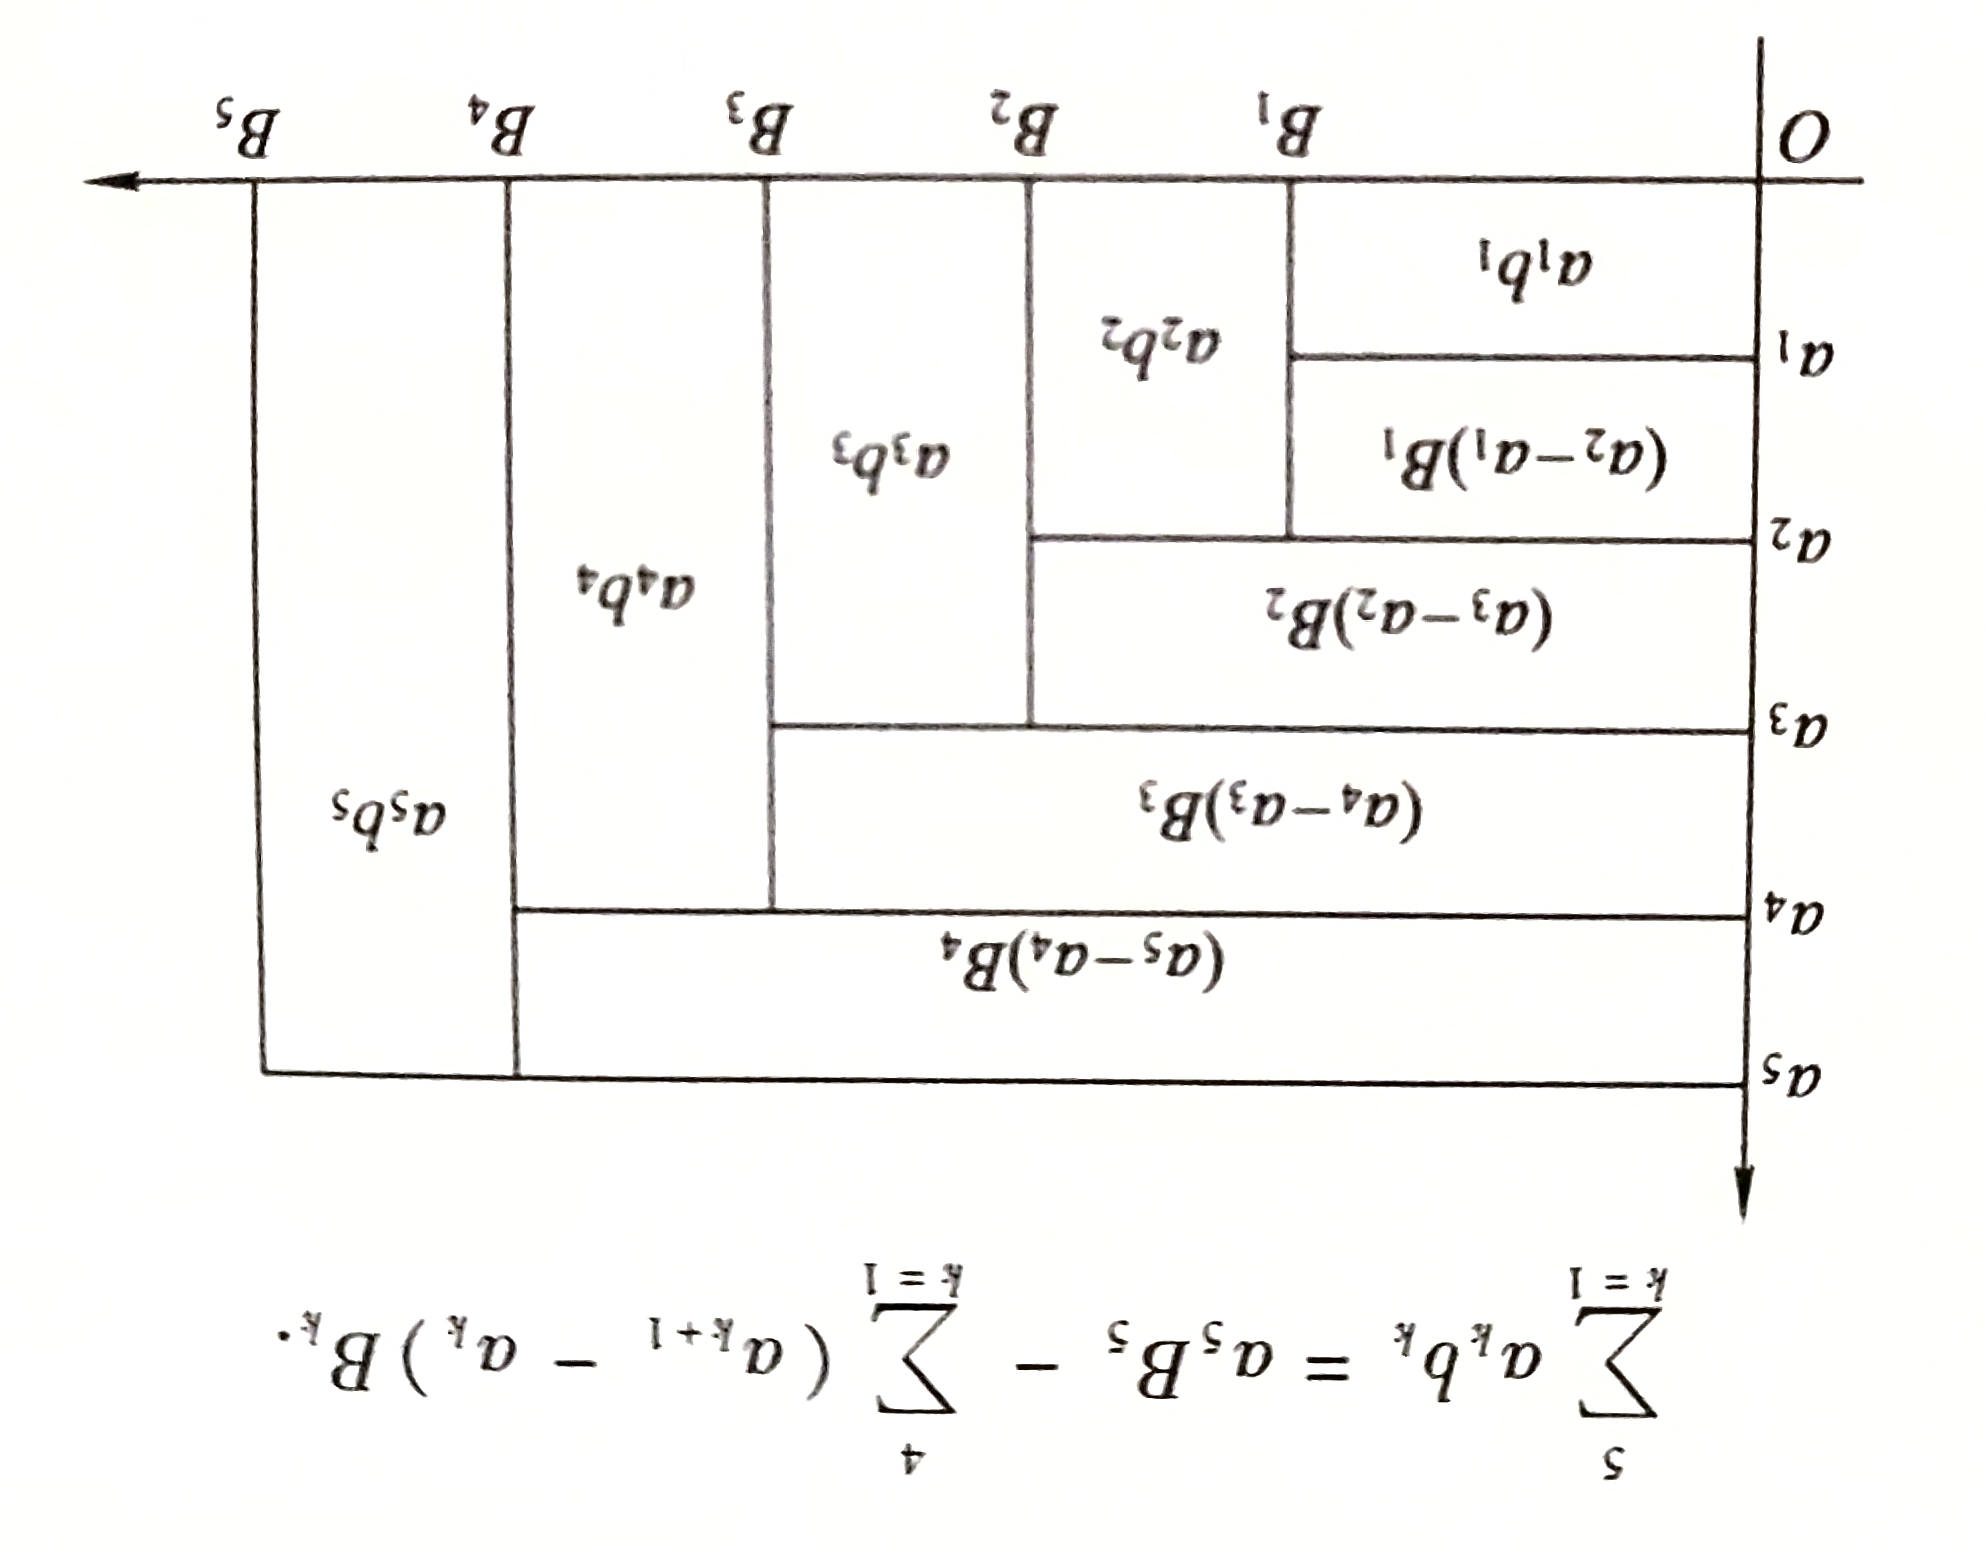
\includegraphics[width=0.5\textwidth, angle=180]{img/AbelTransform.jpg}
\end{figure}

\begin{lemma}{Abel Lemma (Discrete Second Integral Mean Value Theorem)}
    Let \(\{a_n\}, \{b_n\}\) be two sequences, if \(\{a_n\}\) is a monotonic sequence 
    and \(\{B_k\} = \sum_{k=1}^{n} b_k\) is a bounded sequence with bound \(M\),
    then for any \(p\in \mathbb{N}^{+}\),
    \[
        \left| \sum_{k=1}^{p} a_k b_k \right| \leqslant M \left( |a_{1}| + 2|a_{p}| \right) .
    \]
\end{lemma}

\begin{theorem}{Abel-Dirichlet Test}
    The series \(\sum_{n=1}^{\infty} a_n b_n\) converges if one of the following two conditions is satisfied:
    \begin{description}
        \item[Abel] \(\{a_n\}\) is a bounded monotonic sequence and \(\sum_{n=1}^{\infty} b_n\) converges.
        \item[Dirichlet]  \(\{a_n\}\) is a monotonic sequence, \(\lim_{n \to \infty} a_n = 0\),
            and the partial sums \(B_n = \sum_{k=1}^{n} b_k\) are bounded.       
    \end{description}
\end{theorem}

\section{Absolute and Conditional Convergence of Series}
\begin{definition}{Absolute and Conditional Convergence of Series}
    If the series \( \sum_{n=1}^{\infty} |x_n| \) converges, 
    then the series \( \sum_{n=1}^{\infty} x_n \) is said to be \textbf{absolutely convergent}.

    If the series \( \sum_{n=1}^{\infty} x_n \) converges but is not absolutely convergent, 
    then the series \( \sum_{n=1}^{\infty} x_n \) is said to be \textbf{conditionally convergent}.
\end{definition}

\section{Comparison of Convergence Speed of Series}
The series \( \sum_{n=1}^{\infty} a_n \) is said to converge faster than the series \( \sum_{n=1}^{\infty} b_n \) if:
\[
\lim_{n \to \infty} \frac{a_n}{b_n} = 0.
\]

\begin{theorem}{Du Bois-Reymond Theorem}
    For a given convergent positive term series \( \sum_{n=1}^{\infty} a_n \), there always exists a convergent strictly positive term series \( \sum_{n=1}^{\infty} b_n \) such that:
    \[
    \lim_{n \to \infty} \frac{a_n}{b_n} = 0.
    \]
\end{theorem}

\begin{theorem}{Abel Theorem}
    For a given divergent positive term series \( \sum_{n=1}^{\infty} a_n \), there always exists a divergent positive term series \( \sum_{n=1}^{\infty} b_n \) such that:
    \[
    \lim_{n \to \infty} \frac{a_n}{b_n} = 0.
    \]
\end{theorem}

\begin{remark}
    The above two theorems imply that the slowest converging positive term series \underline{does not} exist.
\end{remark}



\section{Infinite Products}
\begin{leftbarTitle}{Infinite Products}\end{leftbarTitle}


\begin{leftbarTitle}{Two Formulas}\end{leftbarTitle}
\begin{theorem}{Wallis Formula}
    \[
    \lim_{n \to \infty} \frac{1}{2n+1} \left[ \frac{(2n)!!}{(2n-1)!!} \right]^{2}  = \frac{\pi}{2}.
    \]
    Equivalently (\(n\to +\infty\)),
    \begin{gather*}
        \frac{(2n)!!}{(2n-1)!!} \sim \sqrt{\pi n}, \\
        \frac{(n!)^{2}2^{2n}}{(2n)!} \sim \sqrt{\pi n}.
    \end{gather*}
\end{theorem}


\begin{theorem}{Stirling Formula}
    \[
    n! = \sqrt{2\pi n} \left( \frac{n}{e} \right)^n 
    \left( 1 + \frac{1}{12n} - \frac{1}{288n^2} + \frac{139}{51840n^3} - \frac{571}{2488320n^4} + \cdots 
    + \frac{B_{2n}}{2k(2k-1) n^{k}} + \cdots  \right),
    \]
    where \( B_{2k} \) are Bernoulli numbers of order \( 2k \).
    Simplified form:
    \[
    n! \sim \sqrt{2\pi n} \left( \frac{n}{e} \right)^{n} \quad (n \to +\infty),
    \]
    or
    \[
    n! = \sqrt{2\pi n} \left( \frac{n}{e} \right)^{n} e^{\theta_n}, \quad \frac{1}{12n+1} < \theta_n < \frac{1}{12n}.
    \]
\end{theorem}


\section{Special Series}

\chapter{Series of Functions}
\section{Pointwise and Uniform Convergence}
\begin{leftbarTitle}{Pointwise Convergence}\end{leftbarTitle}
\begin{definition}{Function Term Series}
    Let \( u_n(x) \) (\( n = 1, 2, 3, \dots \)) be a sequence of functions with a common domain \( E \). 
    The sum of these infinitely many functions \( u_1(x) + u_2(x) + \dots + u_n(x) + \dots \) 
    is called a \textbf{function term series}, denoted as:
    \[
    \sum_{n=1}^{\infty} u_n(x).
    \]

    For any fixed point \( x_0 \in E \), if the numerical series \( \sum_{n=1}^{\infty} u_n(x_0) \) converges, 
    then the function term series \( \sum_{n=1}^{\infty} u_n(x) \) is said to 
    converge at \( x_0 \), or equivalently, \( x_0 \) is called 
    a \textbf{convergence point} of \( \sum_{n=1}^{\infty} u_n(x) \).

    The set of all convergence points is called the \textbf{domain of convergence} of \( \sum_{n=1}^{\infty} u_n(x) \).
\end{definition}

\begin{definition}{Pointwise Convergence}
    Let the domain of convergence of the function term series \( \sum_{n=1}^\infty u_n(x) \) be \( D \subset E \). 
    Then \( \sum_{n=1}^\infty u_n(x) \) defines a function \( S(x) \) on the set \( D \), where:
    \[
    S(x) = \sum_{n=1}^\infty u_n(x), \quad x \in D.
    \]
    The function \( S(x) \) is called the \textbf{sum function} of the series, 
    and \( \sum_{n=1}^\infty u_n(x) \) is said to \textbf{converge pointwise} to \( S(x) \) on \( D \).
\end{definition}

Define the \textbf{partial sum function} of the series as:
\[
S_n(x) = \sum_{k=1}^n u_k(x).
\]
It is evident that the set of all \( x \) for which \( \{ S_n(x) \} \) converges is precisely \( D \). 
Therefore, on \( D \), we have:
\[
S(x) = \lim_{n \to \infty} S_n(x) = \lim_{n \to \infty} \sum_{k=1}^n u_k(x).
\]
Conversely, if a sequence of functions \( \{ S_n(x) \} \) (\( x \in E \)) is given, we can define:
\[
\begin{cases}
u_1(x) = S_1(x), \\
u_{n+1}(x) = S_{n+1}(x) - S_n(x), \quad n = 1, 2, \dots
\end{cases}
\]
to obtain the corresponding function term series.

Thus, the convergence behavior of a function term series and the corresponding sequence 
of partial sum functions is essentially the same.

However, it is important to note that the pointwise convergence has certain limitations.

\begin{description}
    \item[Continuity]
    The sum of finitely many continuous functions satisfies additive continuity:
    \[
    \lim_{x \to x_0} [u_1(x) + u_2(x) + \dots + u_n(x)] 
    = \lim_{x \to x_0} u_1(x) + \lim_{x \to x_0} u_2(x) + \dots + \lim_{x \to x_0} u_n(x).
    \]

    If this property can be extended to infinitely many functions, that is:
    If \( u_n(x) \) is continuous on \( D \), the sum function \( S(x) = \sum_{n=1}^\infty u_n(x) \) 
    is also continuous on \( D \). Moreover:
    \[
    \lim_{x \to x_0} \sum_{n=1}^\infty u_n(x) = \sum_{n=1}^\infty \lim_{x \to x_0} u_n(x),
    \]
    meaning that \underline{the limit operation and infinite summation can be interchanged}
    (also known as the fact that function term series can be evaluated termwise).

    For the sequence of partial sums \( \{ S_n(x) \} \), 
    the corresponding conclusion is that the limit function 
    \( S(x) = \lim_{n \to \infty} S_n(x) \) is also continuous on \( D \), and:
    \[
    \lim_{x \to x_0} \lim_{n \to \infty} S_n(x) = \lim_{n \to \infty} \lim_{x \to x_0} S_n(x),
    \]
    meaning that the two limit operations can be interchanged.

    Unfortunately, in the case of pointwise convergence, this property \textcolor{red!70}{does not hold}.

    \item[Derivability]
    The sum of finitely many differentiable functions satisfies additive differentiability:
    \[
    \frac{\mathrm{d}}{\mathrm{d}x} [u_1(x) + u_2(x) + \dots + u_n(x)] 
    = \frac{\mathrm{d}}{\mathrm{d}x} u_1(x) + \frac{\mathrm{d}}{\mathrm{d}x} u_2(x) + \dots + \frac{\mathrm{d}}{\mathrm{d}x} u_n(x).
    \]

    If this property can be extended to infinitely many functions, that is:
    If \( u_n(x) \) is differentiable on \( D \), 
    the sum function \( S(x) = \sum_{n=1}^\infty u_n(x) \) is also differentiable on \( D \). Moreover:
    \[
    \frac{\mathrm{d}}{\mathrm{d}x} \sum_{n=1}^\infty u_n(x) = \sum_{n=1}^\infty \frac{\mathrm{d}}{\mathrm{d}x} u_n(x),
    \]
    meaning that \underline{the differentiation operation and infinite summation can be interchanged }
    (also known as the fact that function term series can be differentiated termwise).

    For the sequence of partial sums \( \{ S_n(x) \} \), 
    the corresponding conclusion is that the limit function 
    \( S(x) = \lim_{n \to \infty} S_n(x) \) is also differentiable on \( D \), and:
    \[
    \frac{\mathrm{d}}{\mathrm{d}x} \lim_{n \to \infty} S_n(x) = \lim_{n \to \infty} \frac{\mathrm{d}}{\mathrm{d}x} S_n(x),
    \]
    meaning that the two operations can be interchanged.

    Unfortunately, in the case of pointwise convergence, this property \textcolor{red!70}{does not hold}.


    \item[Integrability]
    The sum of finitely many integrable functions satisfies additive integrability:
    \[
    \int_a^b [u_1(x) + u_2(x) + \dots + u_n(x)] \, \mathrm{d}x 
    = \int_a^b u_1(x) \, \mathrm{d}x + \int_a^b u_2(x) \, \mathrm{d}x + \dots + \int_a^b u_n(x) \, \mathrm{d}x.
    \]

    If this property can be extended to infinitely many functions, that is:
    If \( u_n(x) \) is integrable on \( [a, b] \subset D \), 
    the sum function \( S(x) = \sum_{n=1}^\infty u_n(x) \) is also integrable on \( [a, b] \subset D \). Moreover:
    \[
    \int_a^b \sum_{n=1}^\infty u_n(x) \, \mathrm{d}x = \sum_{n=1}^\infty \int_a^b u_n(x) \, \mathrm{d}x,
    \]
    meaning that \underline{the integration operation and infinite summation can be interchanged }
    (also known as the fact that function term series can be integrated termwise).

    For the sequence of partial sums \( \{ S_n(x) \} \), 
    the corresponding conclusion is that the limit function \( S(x) = \lim_{n \to \infty} S_n(x) \) is also integrable on \( [a, b] \subset D \), and:
    \[
    \int_a^b \lim_{n \to \infty} S_n(x) \, \mathrm{d}x = \lim_{n \to \infty} \int_a^b S_n(x) \, \mathrm{d}x,
    \]
    meaning that the two operations can be interchanged.

    Unfortunately, in the case of pointwise convergence, this property \textcolor{red!70}{does not hold}.
\end{description}


\begin{leftbarTitle}{Uniform Convergence}\end{leftbarTitle}
\begin{definition}{Uniform Convergence}
    Let \( \{ S_n(x) \} (x \in D) \) be a sequence of functions. If:
    \[
    \forall \varepsilon > 0, \exists N(\varepsilon) \in \mathbb{N}^+, \forall n > N(\varepsilon): 
    |S_n(x) - S(x)| < \varepsilon \quad (\forall x \in D),
    \]
    then \( \{ S_n \} \) is said to \textbf{converge uniformly} to \( S(x) \) on \( D \), denoted as:
    \[
    S_n(x) \mathop{\rightrightarrows}\limits^{D} S(x).
    \]

    If the partial sum sequence \( \{ S_n(x) \} \) of the function term series 
    \( \sum_{n=1}^\infty u_n(x) (x \in D) \) converges uniformly to \( S(x) \) on \( D \), 
    then \( \sum_{n=1}^\infty u_n(x) \) is said to converge uniformly to \( S(x) \) on \( D \).
\end{definition}
Obviously, if the partial sum sequence \( \{ S_n(x) \} \) of \( \sum_{n=1}^\infty u_n(x) \) satisfies:
\[
S_n(x) \mathop{\rightrightarrows}\limits^{D} S(x),
\]
then:
\[
u_n(x) \mathop{\rightrightarrows}\limits^{D} 0.
\]

\begin{theorem}{Cauchy Criterion for Uniform Convergence}
    The necessary and sufficient condition for the sequence of functions \( \{ S_n(x) \} \) to converge uniformly on \( D \) is:
    \[
    \forall \varepsilon > 0, \exists N \in \mathbb{N}^*, \forall m > n > N: 
    |S_m(x) - S_n(x)| < \varepsilon \quad (\forall x \in D).
    \]

    Correspondingly, the necessary and sufficient condition for the function term series 
    \( \sum_{n=1}^\infty u_n(x) \) to converge uniformly on \( D \) is:
    \[
    \forall \varepsilon > 0, \exists N \in \mathbb{N}^*, \forall m > n > N: 
    \left| \sum_{i=n+1}^m u_i(x) \right| < \varepsilon \quad (\forall x \in D).
    \]
\end{theorem}

\begin{theorem}{Necessary and Sufficient Conditions for Uniform Convergence}
    Let \( \{ S_n(x) \} \) converge pointwise to \( S(x) \) on \( D \). 
    The necessary and sufficient conditions for \( S_n(x) \mathop{\rightrightarrows}\limits^{D} S(x) \) are:
    \begin{enumerate}
        \item  
            \[
            \lim_{n \to \infty} d(S_n, S) = \lim_{n \to \infty} \sup_{x \in D} |S_n(x) - S(x)| = 0.
            \]
        \item For any sequence \( \{ x_n \} \) where \( x_n \in D \), the following holds:
            \[
            \lim_{n \to \infty} \big(S_n(x_n) - S(x_n)\big) = 0.
            \]
    \end{enumerate}
\end{theorem}

With the concept of uniform convergence, the flaws of pointwise convergence can be remedied,
and the following properties can be established:
\begin{property}
    \begin{description}
        \item  [Continuity]
            Let \( f_n(x) \mathop{\rightrightarrows}\limits^{I \subset \mathbb{R}} f(x) \). 
            If \( f_n(x) \) is continuous at \( x_0 \in I \) for \( n = 1, 2, 3, \dots \), 
            then \( f(x) \) is also continuous at \( x_0 \). 

            In particular, if \( f_n(x) \in C(I) \), then \( f(x) \in C(I) \).

            \textbf{Termwise Limit} If \( \sum_{n=1}^\infty u_n(x) \mathop{\rightrightarrows}\limits^{I \subset \mathbb{R}} S(x) \) 
            and \( u_n(x) \in C(I) \), then the sum function \( S(x) \in C(I) \).
        \item  [Integrability]
            Let \( f_n(x) \mathop{\rightrightarrows}\limits^{[a, b]} f(x) \). 
            If \( f_n(x) \in R[a, b] \), then \( f(x) \in R[a, b] \), and:
            \[
            \lim_{n \to \infty} \int_a^b f_n(x) \, \mathrm{d}x = \int_a^b \lim_{n \to \infty} f_n(x) \, \mathrm{d}x = \int_a^b f(x) \, \mathrm{d}x.
            \]

            \textbf{Termwise Integration:} If \( \sum_{n=1}^\infty u_n(x) \mathop{\rightrightarrows}\limits^{[a, b]} S(x) \) 
            and \( u_n(x) \in R[a, b] \), then \( S(x) \in R[a, b] \).

        \item [Differentiability]
            Let \( f'_n(x) \mathop{\rightrightarrows}\limits^{[a, b]} \sigma(x) \). 
            If there exists \( x_0 \in [a, b] \) such that:
            \[
            \lim_{n \to \infty} f_n(x_0) = a,
            \]
            then there exists a function \( f(x) \) such that \( f_n(x) \mathop{\rightrightarrows}\limits^{[a, b]} f(x) \) 
            and \( f'(x) = \sigma(x) \).
            
            \textbf{Termwise Differentiation} If 
            \( \sum_{n=1}^\infty u'_n(x) \mathop{\rightrightarrows}\limits^{[a, b]} \sigma(x) \) 
            and there exists \( x_0 \in [a, b] \) such that:
            \[
            \sum_{n=1}^\infty u_n(x_0) \to a,
            \]
            then there exists a function \( S(x) \) such that 
            \( \sum_{n=1}^\infty u_n(x) \mathop{\rightrightarrows}\limits^{[a, b]} S(x) \) and \( S'(x) = \sigma(x) \).

            \textbf{Corollary} Obviously, if we add the condition \( f'_n(x) \in C[a, b] \), the conclusion still holds, 
            and the proof becomes simpler.
    \end{description}
\end{property}

\begin{note}
    Since continuity and differentiability are both local properties, 
    it suffices to have \textbf{internally closed uniform convergence} of \( (a, b) \) 
    to ensure that \( f(x) \) is continuous/differentiable.
\end{note}


\begin{leftbarTitle}{Quasi-Uniform Convergence}\end{leftbarTitle}
\begin{definition}{Quasi-Uniform Convergence}
    The sequence of functions \( \{ S_n(x) \} \) is said to \textbf{converge quasi-uniformly}
    on the interval \( [a, b] \) 
    if it converges pointwise to \( S(x) \) on \( [a, b] \), and the following condition is satisfied:
    \[
    \forall \varepsilon > 0, \forall N \in \mathbb{N}^*, \exists N_0 > N,
    \text{ s.t. } \forall x \in [a, b], \exists n_x \in [N, N_0] \; 
    (n_x \in \mathbb{N}^*): |S_{n_x}(x) - S(x)| < \varepsilon.
    \]    
\end{definition}


\section{Uniform Convergence Tests}
\begin{leftbarTitle}{Weierstrass Test (M-Test)}\end{leftbarTitle}
\begin{theorem}{Weierstrass Test (M-Test)}
    If there exists a convergent positive term series \( \sum_{n=1}^{\infty} a_n \) such that:
    \[
    |u_n(x)| \leqslant a_n, \quad \forall x \in E, n = 1, 2, 3, \dots
    \]
    then the function term series \( \sum_{n=1}^{\infty} u_n(x) \) converges uniformly on \( E \).

    The positive term series \( \sum_{n=1}^{\infty} a_n \) 
    is called a \textbf{majorant series} of \( \sum_{n=1}^{\infty} u_n(x) \).

    If replace the convergent positive term series \( \sum_{n=1}^{\infty} a_n \)
    with a uniform convergent series of functions \( \sum_{n=1}^{\infty} a_n(x) \),
    the conclusion still holds. 
\end{theorem}


\begin{leftbarTitle}{Abel-Dirichlet Test}\end{leftbarTitle}
\begin{theorem}{Abel-Dirichlet Test}
    If the series of functions \( \sum_{n=1}^{\infty} a_n(x) b_n(x) \) (\(x \in E\)) satisfies 
    at least one of the following two conditions, then it converges uniformly on \( E \).
    \begin{description}
        \item[Abel] \( \{ a_n(x_{0}) \} \) (\(\forall x_{0} \in E\)) is monotonic
            and the series of functions \( \{ a_n(x) \} \) is bounded uniformly on \( E \).
            Simultaneously, the series \( \sum_{n=1}^{\infty} b_n(x) \) converges uniformly on \( E \).
        \item[Dirichlet] \( \{ a_n(x_{0}) \} \) (\(\forall x_{0} \in E\)) is a monotonic and 
            and \( a_n(x) \to 0 \) uniformly convergent on \( E \) with limit \(0\).
            Simultaneously, the partial sums \( B_n(x) = \sum_{k=1}^{n} b_k(x) \) are uniformly bounded on \( E \).
    \end{description}
\end{theorem}

\begin{leftbarTitle}{Dini Theorem}\end{leftbarTitle}
\begin{theorem}{Dini Theorem}
    Let the sequence of functions \( \{ S_n(x) \} \) converges pointwise to \( S(x) \) on the closed interval \( [a, b] \),
    if
    \begin{enumerate}
        \item \( S_n(x) \in C[a, b] \) (\( n = 1, 2, 3, \dots \)); 
        \item \( S(x) \in C[a, b] \);
        \item \(\{ S_{n}(x_{0}) \}\) (\(\forall x_{0} \in [a, b]\)) is monotonic;
    \end{enumerate}
    then \( S_n(x) \mathop{\rightrightarrows}\limits^{[a, b]} S(x) \).
\end{theorem}

\begin{remark}
    Removing the condition of monotonicity, the Arzelà-Borel theorem (~\ref{thm:}) becomes the result of quasi-uniform convergence.
\end{remark}

\section{Special Cases}

\chapter{Power Series}
\section{Power Series and Its Convergence Radius}

\section{Expanding Functions into Power Series}

\section{Smooth Appropriation of Functions}

\chapter{Limits and Continuity in Euclidean Spaces}

\section{Continuous Mappings}
\begin{leftbarTitle}{Continuous Mappings on Compact Sets}\end{leftbarTitle}

\begin{leftbarTitle}{Continuous Mappings on Connected Sets}\end{leftbarTitle}
\begin{definition}{Connected Set}
    Let \(S\) be a set of points in \(\mathbb{R}^n\). 
    If a continuous mapping 
    \[
        \gamma: [0, 1] \to \mathbb{R}^n
    \]
    satisfies that the range of \(\gamma([0, 1])\) lies entirely within \(S\), 
    we call \(\gamma\) a \textbf{path} in \(S\), 
    where \(\gamma(0)\) and \(\gamma(1)\) are referred to as the starting point and ending point of the path, respectively.  
    
    If for any two points \(\mathbf{x}, \mathbf{y} \in S\), 
    there exists a path in \(S\) with \(\mathbf{x}\) as the starting point and \(\mathbf{y}\) as the ending point, 
    \(S\) is called path-connected, or equivalently, \(S\) is called a \textbf{connected set}.  
    
    A connected open set is called an \textbf{(open) region}. The closure of an (open) region is referred to as a closed region.
\end{definition}

\begin{remark}
    Intuitively, this means that any two points in \(S\) can be connected 
    by a curve lying entirely within \(S\). 
    Clearly, a connected subset of \(\mathbb{R}\) is an interval, 
    and a connected subset of \(\mathbb{R}\) is compact if and only if it is a closed interval.
\end{remark}



\chapter{Multi-variable Differential Calculus}
\section{Directional Derivatives and Total Differential}
\begin{leftbarTitle}{Directional Derivative}\end{leftbarTitle}
\begin{definition}{Directional Derivative}
    Let \(U\subset \mathbb{R}^n\) be an open set, \(f: U\to \mathbb{R}^{1}\),
    \(\mathbf{e}\) is a unit vector in \(\mathbb{R}^{n}\), \(\mathbf{x}^{0}\in U\). Define
    \[
    u(t) = f(\mathbf{x}^{0} + t\mathbf{e}).
    \]
    If the derivative of \(u\) at \(t=0\) 
    \[ 
        u'(0) = \lim_{t \to 0} \frac{u(t) - u(0)}{t} = 
        \lim_{t \to 0} \frac{f(\mathbf{x}^{0} + t\mathbf{e}) - f(\mathbf{x}^{0})}{t} 
    \] 
    exists and is finite, 
    it is called the \textbf{directional derivative} of \(f\) at \(\mathbf{x}^{0}\) in the direction \(\mathbf{e}\), 
    denoted by \(\frac{\partial f}{\partial \mathbf{e}}(\mathbf{x}^{0})\). 
    It is the rate of change of \(f\) at \(\mathbf{x}^{0}\) in the direction \(\mathbf{e}\).
\end{definition}

Consider the following set of unit coordinate vectors: \(\mathbf{e}_{1},\mathbf{e}_{2},\cdots,\mathbf{e}_{n}\).
Let \(\mathbf{e}_{i}=\left( 0, 0, \cdots, 0, 1, 0, \cdots, 0 \right)  \) denote the standard orthonormal basis 
in \(\mathbb{R}^{n}\), where the 1 appears in the \(i\)-th position. That is,
\[
    \langle \mathbf{e}_{i}, \mathbf{e}_{j} \rangle = \delta_{i j} = \begin{cases}
    1, & i = j, \\
    0, & i \neq j.
    \end{cases}
\]
For a function \( f \), the directional derivative of \( f \) at the point \( \mathbf{x}_{0} \) 
in the direction of \( \mathbf{e}_{i} \) 
is called the \( i \)th first-order \textbf{partial derivative} of \( f \) at \(\mathbf{x}^{0}\), denoted by
\[
\frac{\partial f}{\partial x_i}(\mathbf{x}^{0}) \quad \text{or} 
\quad \mathrm{D}_i f(\mathbf{x}^{0})  \quad \text{or} 
\quad f_{x_i}(\mathbf{x}^{0}) \quad (i = 1, 2, \cdots, n).
\]
\( \mathrm{D}_i = \frac{\partial}{\partial x_i} \) is called the \( i \)th partial differential operator (\( i = 1, 2, \cdots, n \)).

Let \(\mathbf{e}_{i}=\sum_{i=0}^{n} \mathbf{e}_{i}\cos\alpha\) be a unit vector, 
where \(\sum_{i=0}^{n} \cos^2\alpha = 1\).
If \(\frac{\partial f}{\partial x_{i}}\) is continuous at \(\mathbf{x}^0\), 
then the directional derivative of \(f\) at \(\mathbf{x}^0\) along the direction \(\mathbf{e}\) is given by:
\[
\frac{\partial f}{\partial \mathbf{e}}(\mathbf{x}^0) = \sum_{i=1}^n \frac{\partial f}{\partial x_i}(\mathbf{x}^0) \cos \alpha_i.
\]

This is the formula for \textbf{expressing a directional derivative using partial derivatives}.


\begin{note}
    Let \(\mathbf{e}\) be a direction, then \(\|-\mathbf{e}\| = \|\mathbf{e}\| = 1\), 
    which implies that \(-\mathbf{e}\) is also a direction. At this point, we have:
    \[
    \frac{\partial f}{\partial (-\mathbf{e})}(\mathbf{x}^{0}) = -\frac{\partial f}{\partial \mathbf{e}}(\mathbf{x}^{0}).
    \]
\end{note}



\begin{definition}{Jacobian Matrix (Gradient)}
    Let
    \[
    Jf(\mathbf{x}) = (\mathrm{D}_1 f(\mathbf{x}), \mathrm{D}_2 f(\mathbf{x}), \dots, \mathrm{D}_n f(\mathbf{x})),
    \]
    which is called the \textbf{Jacobian matrix} of the function \( f \) at the point \( \mathbf{x} \), 
    (a \( 1 \times n \) matrix) whose counterpart is the first-order derivative of a single-variable function.

    Henceforth, we represent the point \(\mathbf{x}\) in \( \mathbb{R}^n \) 
    and its increments \(\mathbf{h}\) as column vectors.
    In this way, the differential of the function can be expressed using matrix multiplication as follows:
    \[
    \mathrm{d}f(\mathbf{x}^{0})(\mathbf{\Delta x}) = Jf(\mathbf{x}^{0}) \mathbf{\Delta x}.
    \]
    The Jacobian matrix of the function \( f \) is also frequently denoted as 
    \(\mathrm{grad}\,f\) (or \(\nabla f\)), that is,
    \[
    \mathrm{grad}\,f(\mathbf{x}) = Jf(\mathbf{x}),
    \]
    which is called the \textbf{gradient} of the scalar function \( f \).
\end{definition}



\begin{leftbarTitle}{Total Differential}\end{leftbarTitle}
\begin{definition}{Total Differential}
    Let \(U\subset \mathbb{R}^n\) be an open set, \(f: U\to \mathbb{R}^{1}\), \(\mathbf{x}^{0}\in U\),
    \(\mathbf{\Delta x}=\left( \Delta x_{1},\Delta x_{2},\cdots,\Delta x_{n} \right) \in \mathbb{R}^{n}\). If
    \[
    f(\mathbf{x}^{0} + \mathbf{\Delta x}) - f(\mathbf{x}^{0}) = 
    \sum_{i=1}^n A_{i} \Delta x_{i} + o(\|\mathbf{\Delta x}\|) \qquad (\|\mathbf{\Delta x}\| \to 0),
    \]
    where \(A_{1}, A_{2}, \dots, A_{n}\) are constants independent of \(\mathbf{\Delta x}\), 
    then the function \(f\) is said to be \textbf{differentiable} at the point \(\mathbf{x}^{0}\), 
    and the linear main part \(\sum_{i=1}^n A_{i} \Delta x_{i}\) is called the \textbf{total differential} 
    of \(f\) at \(\mathbf{x}^{0}\), 
    denoted as
    \[
    df(\mathbf{x}^{0})(\mathbf{\Delta x}) = \sum_{i=1}^n A_{i} \Delta x_{i}.
    \]
    If \(f\) is differentiable at every point in the open set \(U\), 
    then \(f\) is called a differentiable function on \(U\).    
\end{definition}

\begin{theorem}{Conditions of Differentiability}
    \begin{description}
        \item[Necessary Condition] If an \(n\)-variable function \(f\) is differentiable at the point \(\mathbf{x}_{0}\), 
        then \(f\) is continuous at \(\mathbf{x}^{0}\) and 
        possesses first-order partial derivatives \(\frac{\partial f}{\partial x_{i}}(\mathbf{x}^{0})\) 
        at \(\mathbf{x}^{0}\) for \(i = 1, 2, \dots, n\), and
        \[
        \mathbf{A} = \left( A_{1}, A_{2}, \dots, A_{n} \right)  = Jf(\mathbf{x}^{0}) = 
        \left(\mathrm{D}_{1}f(\mathbf{x}^{0}), \mathrm{D}_{2}f(\mathbf{x}^{0}), \dots, \mathrm{D}_{n}f(\mathbf{x}^{0}) \right).
        \]\footnote{
            It is referred to as the total differential formula, and the more common form is
            \[
                \mathrm{d}f(x_{0},y_{0})=
                \frac{\partial f}{\partial x}(x_{0},y_{0})\,\mathrm{d}x+\frac{\partial f}{\partial y}(x_{0},y_{0})\,\mathrm{d}y.
            \]
        }
        However, the converse is not true.
        %%%%%%%%%%%%%%%%%%%%%%%%%%%%%%%%%%%%%%%%%%%%%%%%%%%%%%%%%%%%%%%%%%%%%%%%%%%%%%%%%%%%%%%%%
        \item[Sufficient Condition] Let \(U \subset \mathbb{R}^n\) be an open set, 
        and let \(f: U \to \mathbb{R}^1\) be an \(n\)-variable function. 
        If \(Jf = \left( \mathrm{D}_{1}f, \mathrm{D}_{2}f, \dots, \mathrm{D}_{n}f \right)\) 
        is continuous at \(\mathbf{x}^{0}\) 
        (i.e., \(\frac{\partial f}{\partial x_{i}}\) is continuous at \(\mathbf{x}^{0}\) for \(i = 1, 2, \dots, n\)), 
        then \(f\) is differentiable at \(\mathbf{x}^{0}\).
        However, the converse is not necessarily true.
    \end{description}    
\end{theorem}

\begin{note}
    \begin{itemize}
        \item The continuity of the derivative function at \(\mathbf{x}^{0}\) implies that 
            the original function \(f\) is differentiable in some neighborhood of \(\mathbf{x}^{0}\).
        \item In fact, this condition can be relaxed to require that one partial derivative exists at the point, 
            while the remaining \(n-1\) partial derivative functions are continuous at that point.
    \end{itemize}
\end{note}

\begin{proof}
    Taking a function of three variables as an example.

    Assume the \(3\)-ary function \(f: \mathbb{R}^3 \to \mathbb{R}\) meets:
    \begin{enumerate}
        \item There exists \(f_{z}(x_{0},y_{0},z_{0})\). 
        \item The partial derivative functions \(f_{x}(x,y,z)\) and \(f_{y}(x,y,z)\) are continuous at \((x_{0},y_{0},z_{0})\),
            i.e. there are partial derivatives in some neighborhood of \((x_{0},y_{0},z_{0})\).
    \end{enumerate}
    Consider the total increment of \(f\) at the point \((x_{0},y_{0},z_{0})\):
    \begin{align*}
        \Delta f 
        &= \underbrace{\left[ f(x_0 + \Delta x, y_0 + \Delta y, z_0 + \Delta z) - f(x_0, y_0 + \Delta y, z_0 + \Delta z) \right]}_{I_1}\\
        &+ \underbrace{\left[ f(x_0, y_0 + \Delta y, z_0 + \Delta z) - f(x_0, y_0, z_0 + \Delta z) \right]}_{I_2}\\
        &+ \underbrace{\left[ f(x_0, y_0, z_0 + \Delta z) - f(x_0, y_0, z_0) \right]}_{I_3}.
    \end{align*}
    For \(I_{1}, I_{2}\), by the Lagrange's Mean Value Theorem of unary functions, 
    there exist \(\theta_{1}, \theta_{2} \in (0,1)\) such that
    \begin{gather*}
        I_{1}=f_{x}(x_{0}+\theta_{1}\Delta x,y_{0}+\Delta y,z_{0}+\Delta z)\Delta x,\\
        I_{2}=f_{y}(x_{0},y_{0}+\theta_{2}\Delta y,z_{0}+\Delta z)\Delta y.
    \end{gather*}
    Then by the continuity of the their partial derivatives at \((x_{0},y_{0},z_{0})\), we have
    \[
        \lim_{\Delta x, \Delta y, \Delta z \to 0} I_{1} = f_{x}(x_{0},y_{0},z_{0})\Delta x, \quad
        \lim_{\Delta x, \Delta y, \Delta z \to 0} I_{2} = f_{y}(x_{0},y_{0},z_{0})\Delta y.
    \]
    They can be expressed in terms of infinitesimals(\(\rho = \sqrt{\Delta x^2 + \Delta y^2 + \Delta z^2}\)):
    \begin{align*}
        I_{1}=f_{x}(x_{0},y_{0},z_{0})\Delta x + \alpha_{1}\Delta x, \quad \alpha_{1}\to 0(\rho\to 0),\\
        I_{2}=f_{y}(x_{0},y_{0},z_{0})\Delta y + \alpha_{2}\Delta y, \quad \alpha_{2}\to 0(\rho\to 0).
    \end{align*}
    For \(I_{3}\), by the definition of the partial derivative \(f_{z}(x,y,z)\) at \((x_{0},y_{0},z_{0})\), we have
    \[
        I_{3}=f_{z}(x_{0},y_{0},z_{0})\Delta z + \alpha_{3}\Delta z, \quad \alpha_{3}\to 0(\rho\to 0).
    \]
    Accordingly, 
    \begin{align*}
        \Delta f &= I_{1} + I_{2} + I_{3} \\
        &= \left[ f_{x}(x_{0},y_{0},z_{0})\Delta x + \alpha_{1}\Delta x \right] + \left[ f_{y}(x_{0},y_{0},z_{0})\Delta y + \alpha_{2}\Delta y \right] + \left[ f_{z}(x_{0},y_{0},z_{0})\Delta z + \alpha_{3}\Delta z \right] \\
        &= f_{x}(x_{0},y_{0},z_{0})\Delta x + f_{y}(x_{0},y_{0},z_{0})\Delta y + f_{z}(x_{0},y_{0},z_{0})\Delta z + \left[ \alpha_{1}\Delta x + \alpha_{2}\Delta y + \alpha_{3}\Delta z \right].
    \end{align*}
    Apparently, 
    \[
        \lim_{\rho \to 0} \frac{\alpha_{1}\Delta x + \alpha_{2}\Delta y + \alpha_{3}\Delta z}{\rho} = 0,
    \]
    i.e. \(\alpha_{1}\Delta x + \alpha_{2}\Delta y + \alpha_{3}\Delta z = o(\rho)\). 
    Therefore, \(f(x,y,z)\) is differentiable at \((x_{0},y_{0},z_{0})\), which completes the proof.
\end{proof}

\begin{note}{(At some point)}
    \begin{enumerate}
        \item  Differentiable
            \begin{itemize}
                \item \(\implies\) Continuous
                \item \(\implies\) Partial derivatives exist: \(\mathrm{D}_{\vec{u}}=\nabla f\cdot\vec{u}\)
            \end{itemize}
        \item  Directional Derivative
            \begin{itemize}
                \item All directional derivatives exist \(\not\implies\) differentiable or continuous.
                \item All directional derivatives exist and are equal \(\not\implies\) differentiable.
            \end{itemize}
        \item  Partial Derivative
        \begin{itemize}
            \item  The continuity and existence of directional/partial derivatives are mutually exclusive.
        \end{itemize}
    \end{enumerate}
\end{note}


\begin{leftbarTitle}{Higher-Order Partial Derivatives and Differential}\end{leftbarTitle}
If the first-order partial derivative of \(f\), \(\frac{\partial f}{\partial x_i}\), 
itself possesses partial derivatives, then the second-order partial derivative of \(f\) is defined, 
and is denoted as follows(the first is also called the mixed partial derivative):
\[
f_{x_i x_j} = \frac{\partial^2 f}{\partial x_i \partial x_j} = \frac{\partial}{\partial x_j} \left( \frac{\partial f}{\partial x_i} \right), 
\quad f_{x_i x_i} = \frac{\partial^2 f}{\partial x_i^2} = \frac{\partial}{\partial x_i} \left( \frac{\partial f}{\partial x_i} \right), 
\quad i, j = 1, 2, \dots, n.
\]

Similarly, higher-order partial derivatives of order \(3,4,\cdots m,\cdots\) can be defined.

The following theorem provides the conditions under which mixed partial derivatives are equal.

\begin{theorem}{Conditions for Equality of Mixed Partial Derivatives}
    \begin{enumerate}\label{thm:condition_equality}
        \item Let $U \subset \mathbb{R}^2$ be an open set, and $f: U \to \mathbb{R}$ be a function of two variables. 
            If $f_{xy}$ and $f_{yx}$ are continuous at $(x_0, y_0) \in U$, then
            \[
            f_{xy}(x_0, y_0) = f_{yx}(x_0, y_0).
            \]
        \item Let \(U \subset \mathbb{R}^n\) be an open set, and \(f: U \to \mathbb{R}\) be a function of \(n\) variables. 
            If \(f\) has partial derivatives up to order \(k\) in \(D\), 
            and all of them are continuous at \(\mathbf{x}^{0} = (x_1^0, x_2^0, \ldots, x_n^0) \in U\), then
                \[
                \frac{\partial^l f}{\partial x_{i_1} \partial x_{i_2} \cdots \partial x_{i_l}}(\mathbf{x}^{0}) 
                = \frac{\partial^l f}{\partial x_{i_2} \partial x_{i_1} \cdots \partial x_{i_l}}(\mathbf{x}^{0}) 
                = \cdots 
                = \frac{\partial^l f}{\partial x_{i_l} \partial x_{i_l - 1} \cdots \partial x_{i_1}}(\mathbf{x}^{0}),
                \]
            that is, the order of taking partial derivatives \(l ( \leqslant k )\) does not affect the result.\footnote{
                If the condition "\(f_{xy}\) and \(f_{yx}\) are continuous at \((x_0, y_0)\)",
                is not satisfied, then the conclusion "\(f_{xy}(x_0, y_0) = f_{yx}(x_0, y_0)\)" does not necessarily hold.
            }
    \end{enumerate}
\end{theorem}


\begin{proof}
    When $k \neq 0, h \neq 0$, define
    \[
        \varphi(y) = f(x_0 + h, y) - f(x_0, y),
    \]
    and
    \[
        \psi(x) = f(x, y_0 + k) - f(x, y_0).
    \]
    Applying the Lagrange Mean Value Theorem, we have
    \[
        \begin{aligned}
            &[f(x_0 + h, y_0 + k) - f(x_0, y_0 + k)] - [f(x_0 + h, y_0) - f(x_0, y_0)] \\
            =& \varphi(y_0 + k) - \varphi(y_0) \\
            =& \varphi'(y_0 + \theta_1 k) k \\
            =& [f_y(x_0 + h, y_0 + \theta_1 k) - f_y(x_0, y_0 + \theta_1 k)] k \\
            =& f_{yx}(x_0 + \theta_2 h, y_0 + \theta_1 k) h k, \quad 0 < \theta_1, \theta_2 < 1.
        \end{aligned}
    \]
    On the other hand,
    \[
        \begin{aligned}
            &[f(x_0 + h, y_0 + k) - f(x_0, y_0 + k)] - [f(x_0 + h, y_0) - f(x_0, y_0)] \\
            =& [f(x_0 + h, y_0 + k) - f(x_0 + h, y_0)] - [f(x_0, y_0 + k) - f(x_0, y_0)] \\
            =& \psi(x_0 + h) - \psi(x_0) \\
            =& \psi'(x_0 + \theta_3 h) h \\
            =& [f_x(x_0 + \theta_{3}h, y_0 + k) - f_x(x_0 + \theta_{3}h, y_0)] h \\
            =& f_{xy}(x_0 + \theta_3 h, y_0 + \theta_4 k) h k, \quad 0 < \theta_3, \theta_4 < 1.
        \end{aligned}
    \]
    Therefore,
    \[
    f_{xy}(x_0 + \theta_3 h, y_0 + \theta_4 k) = f_{yx}(x_0 + \theta_2 h, y_0 + \theta_1 k).
    \]
    Since $f_{xy}$ and $f_{yx}$ are continuous at $(x_0, y_0)$, letting $h \to 0, k \to 0$, we obtain
    \[
    f_{xy}(x_0, y_0) = f_{yx}(x_0, y_0).
    \]
    By applying ~\ref{thm:condition_equality} and the principle of mathematical induction, one can immediately derive the following result.
\end{proof}

Suppose \(z=f(x,y)\) has continuous partial derivatives in the domain \(U\subset \mathbb{R}^2\). 
Then \(z\) is differentiable, and
\[
    \mathrm{d}z = \frac{\partial z}{\partial x} \mathrm{d}x + \frac{\partial z}{\partial y} \mathrm{d}y.
\]
If \(z\) also has continuous second-order partial derivatives, 
then \(\frac{\partial z}{\partial x}\) and \(\frac{\partial z}{\partial y}\) are also differentiable, 
and thus \(\mathrm{d}z\) is differentiable. 
We call the differential of \(\mathrm{d}z\) the second-order differential of \(z\), denoted as
\[
    \mathrm{d}^2z = \mathrm{d}(\mathrm{d}z).
\]
In general, based on the \(k\)-th order differential \(\mathrm{d}^kz\) of \(z\), 
its \((k+1)\)-th order differential (if it exists) is defined as
\[
    \mathrm{d}^{k+1}z = \mathrm{d}(\mathrm{d}^kz), \quad k = 1, 2, \cdots .
\]
Due to the fact that for the independent variables \( x \) and \( y \), we always have
\[
    \mathrm{d}^2 x = \mathrm{d}(\mathrm{d}x) = 0, \qquad \mathrm{d}^2 y = \mathrm{d}(\mathrm{d}y) = 0,
\]
the second-order differential of \( z = f(x, y) \) is given by
\begin{align*}
    \mathrm{d}^2 z &= \mathrm{d}(\mathrm{d}z) 
        = \mathrm{d}\left( \frac{\partial z}{\partial x} \mathrm{d}x + \frac{\partial z}{\partial y} \mathrm{d}y \right) \\
    &= \mathrm{d}\left( \frac{\partial z}{\partial x} \right) \mathrm{d}x + \frac{\partial z}{\partial x} \mathrm{d}^2 x 
        + \mathrm{d}\left( \frac{\partial z}{\partial y} \right) \mathrm{d}y + \frac{\partial z}{\partial y} \mathrm{d}^2 y\\
    &= \left( \frac{\partial^2 z}{\partial x^2} \mathrm{d}x + \frac{\partial^2 z}{\partial x \partial y} \mathrm{d}y \right) \mathrm{d}x
        + \left( \frac{\partial^2 z}{\partial y \partial x} \mathrm{d}x + \frac{\partial^2 z}{\partial y^2} \mathrm{d}y \right) \mathrm{d}y\\
    &= \frac{\partial^2 z}{\partial x^2} (\mathrm{d}x)^2 + 2 \frac{\partial^2 z}{\partial x \partial y} \mathrm{d}x \mathrm{d}y + \frac{\partial^2 z}{\partial y^2} (\mathrm{d}y)^2,
\end{align*}
where \( (\mathrm{d}x)^2 \) and \( (\mathrm{d}y)^2 \) denote \( \mathrm{d}^2 x \) and \( \mathrm{d}^2 y \) respectively.
If we treat \( \frac{\partial}{\partial x} \), \( \frac{\partial}{\partial y} \) as operators for partial differentiation 
and define
\[
    \left( \frac{\partial}{\partial x} \right)^2 = \frac{\partial^2}{\partial x^2}, \quad
    \left( \frac{\partial}{\partial y} \right)^2 = \frac{\partial^2}{\partial y^2}, \quad
    \left( \frac{\partial}{\partial x} \frac{\partial}{\partial y} \right) = \frac{\partial^2}{\partial x \partial y},
\]
then the formulas for the first and second differentials can be written as
\[
    \mathrm{d}z = \left( \mathrm{d}x \frac{\partial}{\partial x} + \mathrm{d}y \frac{\partial}{\partial y} \right) z,
\]
\[
    \mathrm{d}^2 z = \left( \mathrm{d}x \frac{\partial}{\partial x} + \mathrm{d}y \frac{\partial}{\partial y} \right)^2 z.
\]
Similarly, we define
\[
    \left( \frac{\partial}{\partial x} \right)^p
    \left( \frac{\partial}{\partial y} \right)^q
    = \frac{\partial^{p+q}}{\partial x^p \partial y^q}
    = \frac{\partial^q}{\partial y^q}
    \left( \frac{\partial}{\partial x} \right)^p,
    \quad (p, q = 1, 2, \dots)
\]
It is easy to use mathematical induction to prove the formula for higher-order differentials:
\[
    \mathrm{d}^k z = \left( \mathrm{d}x \frac{\partial}{\partial x} + \mathrm{d}y \frac{\partial}{\partial y} \right)^k z, 
    \quad k = 1, 2, \cdots.
\]
For an \( n \)-variable function \( u = f(x_1, x_2, \dots, x_n) \), higher-order differentials can be similarly defined, and the following holds:
\[
    \mathrm{d}^k u 
    = \left( \mathrm{d}x_1 \frac{\partial}{\partial x_1} + \mathrm{d}x_2 \frac{\partial}{\partial x_2} 
    + \cdots + \mathrm{d}x_n \frac{\partial}{\partial x_n} \right)^k u, \quad k = 1, 2, \dots.
\]



\section{Differential of Vector-Valued Functions}
Consider an $n$-dimensional vector-valued function defined on a domain $U \subset \mathbb{R}^n$:
\begin{gather*}
    f: U \to \mathbb{R}^m, \\ 
    \mathbf{x} \mapsto \mathbf{y} = f(\mathbf{x})
\end{gather*}
Expressed in coordinate vector form:
\[
    \mathbf{y} =
    \begin{pmatrix}
    y_1 \\ y_2 \\ \vdots \\ y_m
    \end{pmatrix}
    =
    \begin{pmatrix}
    f_1(x_1, x_2, \dots, x_n) \\
    f_2(x_1, x_2, \dots, x_n) \\
    \vdots \\
    f_m(x_1, x_2, \dots, x_n)
    \end{pmatrix},
    \qquad \mathbf{x} = \begin{pmatrix} 
    x_1 \\ x_2 \\ \vdots \\ x_n 
    \end{pmatrix}  \in U
\]

\begin{enumerate}
    \item  If each component function $f_i(x_1, x_2, \dots, x_n)$ ($i=1,2,\dots,m$) is partially differentiable at $\mathbf{x}^0$, 
        then the vector-valued function $\mathbf{f}$ is differentiable at $\mathbf{x}^0$, and we define the matrix
        \[
            \left( \frac{\partial f}{\partial x_j} (\mathbf{x}^0) \right)_{m \times n}
            =
            \begin{pmatrix}
            \frac{\partial f_1}{\partial x_1}(\mathbf{x}^0) & \frac{\partial f_1}{\partial x_2}(\mathbf{x}^0) & \cdots & \frac{\partial f_1}{\partial x_n}(\mathbf{x}^0) \\
            \frac{\partial f_2}{\partial x_1}(\mathbf{x}^0) & \frac{\partial f_2}{\partial x_2}(\mathbf{x}^0) & \cdots & \frac{\partial f_2}{\partial x_n}(\mathbf{x}^0) \\
            \vdots & \vdots & \ddots & \vdots \\
            \frac{\partial f_m}{\partial x_1}(\mathbf{x}^0) & \frac{\partial f_m}{\partial x_2}(\mathbf{x}^0) & \cdots & \frac{\partial f_m}{\partial x_n}(\mathbf{x}^0)
            \end{pmatrix}
        \]

        This matrix is called the Jacobian matrix of $\mathbf{f}$ at $\mathbf{x}^0$, 
        denoted by $f'(\mathbf{x}^0)$ (or $\mathrm{D}f(\mathbf{x}^0)$, $J_f(\mathbf{x}^0)$).

        For the special case $m=1$, i.e., $n$-variable scalar function $z=f(x_1,x_2,\dots,x_n)$, 
        the derivative at $\mathbf{x}^0$ is
        \[
            f'(\mathbf{x}^0) = 
            \left( 
                \frac{\partial f}{\partial x_1}(\mathbf{x}^0), \frac{\partial f}{\partial x_2}(\mathbf{x}^0), 
                \cdots, \frac{\partial f}{\partial x_n}(\mathbf{x}^0) 
            \right)
        \]
        If the vector-valued function $\mathbf{f}$ is differentiable at every point in $U$, 
        then $\mathbf{f}$ is said to be differentiable on $U$, and the corresponding relationship is
        \[
        \mathbf{x} \in U \mapsto f'(\mathbf{x}) = J_f(\mathbf{x})
        \]
        where $f'(\mathbf{x})$ (or $\mathrm{D}f(\mathbf{x})$, $J_f(\mathbf{x})$) 
        denotes the derivative of $\mathbf{f}$ at $\mathbf{x}$ in $U$.
    \item  If every component function $f_i(x_1, x_2, \dots, x_n)$ $(i=1,2,\dots,m)$ of $\mathbf{f}$ 
        has continuous partial derivatives at $\mathbf{x}^0$, 
        then every element of the Jacobian matrix of $\mathbf{f}$ is continuous at $\mathbf{x}^0$. 
        In this case, $\mathbf{f}$ is said to have a continuous derivative at $\mathbf{x}^0$ as a vector-valued function.
        
        If the derivative of a vector-valued function $\mathbf{f}$ is continuous at every point in $U$, 
        then $\mathbf{f}$ is said to have a continuous derivative on $U$.
    \item  If there exists an $m \times n$ matrix $A$ that depends only on $\mathbf{x}^0$ (and not on $\Delta \mathbf{x}$), 
        such that in the neighborhood of $\mathbf{x}^0$,
        \[
        \Delta \mathbf{y} = f(\mathbf{x}^0 + \Delta \mathbf{x}) - f(\mathbf{x}^0) = A \Delta \mathbf{x} + o(\|\Delta \mathbf{x}\|)
        \]
        (where $\Delta \mathbf{x} = (\Delta x_1, \Delta x_2, \dots, \Delta x_n)^T$ is a column vector and 
        $\|\Delta \mathbf{x}\|$ denotes its norm), 
        then $f$ is said to be differentiable at $\mathbf{x}^0$ as a vector-valued function, 
        and $A\Delta \mathbf{x}$ is called the differential of $f$ at $\mathbf{x}^0$, denoted as $\mathrm{d}\mathbf{y}$. 
        If we denote $\Delta \mathbf{x}$ by 
        $\mathrm{d}\mathbf{x}$ ($\mathrm{d}\mathbf{x} = (\mathrm{d}x_1, \mathrm{d}x_2, \dots, \mathrm{d}x_n)^T$), then
        \[
            \mathrm{d}\mathbf{y} = A\,\mathrm{d}\mathbf{x}.
        \]

        If the vector-valued function $\mathbf{f}$ is differentiable at every point in $U$, 
        then $\mathbf{f}$ is said to be differentiable on $U$.
\end{enumerate}

Combining the above three points, we obtain the following unified statement:

A vector-valued function \(\mathbf{f}\) is continuous, differentiable, 
and has derivatives if and only if each of its coordinate component functions 
\(f_i(x_1, x_2, \dots, x_n)\) (\(i = 1, 2, \dots, m\)) is continuous, differentiable, and has derivatives.


\section{Derivatives of Composite Mappings (Chain Rule)}
Let \( U \subset \mathbb{R}^l \) and \( V \subset \mathbb{R}^n \) be open sets, and let 
\[
\mathbf{g}: U \to V \quad \text{and} \quad \mathbf{f}: V \to \mathbb{R}^m
\]
be mappings. If \( \mathbf{g} \) is derivative at \( \mathbf{u}^{0} \in U \) 
and \( \mathbf{f} \) is differentiable at \( \mathbf{x}^{0} = \mathbf{g}(\mathbf{u}^{0}) \), 
then the composite mapping \( \mathbf{f} \circ \mathbf{g} \) is differentiable at \( \mathbf{u}^{0} \), and:
\[
J(\mathbf{f} \circ \mathbf{g})(\mathbf{u}^{0}) = 
J\mathbf{f}(\mathbf{x}^{0}) J\mathbf{g}(\mathbf{u}^{0}).
\]

\begin{note}
    \begin{enumerate}
        \item  outer differentiable + inner derivative = total derivative
        \item  outer differentiable + inner differentiable = total differentiable
        \item  
    \end{enumerate}
\end{note}

Specially, define \( z = f(x, y), (x,y)\subset D_{f}\subset \mathbb{R}^{2} \), 
\(\mathbf{g}:D_{g}\to \mathbb{R}^{2}, (u,v)\mapsto (x(u,v), y(u,v))\), 
and \(g(D_{g})\subset D_{f}\), 
then we have composite function
\[
z = f \circ \mathbf{g} = f\left[x(u,v), y(u,v)\right],\quad (u,v)\in D_{g}.
\]
\[
\mathbb{R}^{2}\xrightarrow{\mathbf{g}:\text{derivative}}\mathbb{R}^{2}\xrightarrow{f:\text{differentiable}}\mathbb{R}
\]
If \(\mathbf{g}\) is derivative at \((u_{0}, v_{0})\in D_{g}\), 
and \(f\) is differentiable at \((x_{0}, y_{0}) = \mathbf{g}(u_{0}, v_{0})\), 
then \(z = f \circ \mathbf{g}\) is differentiable at \((u_{0}, v_{0})\), and at the point,
\[
    \begin{bmatrix} 
        \frac{\partial z}{\partial u}   & \frac{\partial z}{\partial v} 
    \end{bmatrix} 
    =
    \begin{bmatrix}
        \frac{\partial z}{\partial x} & \frac{\partial z}{\partial y}
    \end{bmatrix}
    \begin{bmatrix} 
        \frac{\partial x}{\partial u} & \frac{\partial x}{\partial v} \\
        \frac{\partial y}{\partial u} & \frac{\partial y}{\partial v}
    \end{bmatrix} 
\]

\begin{proof}
    
\end{proof}

\section{Mean Value Theorem and Taylor's Formula}

\begin{definition}{Convex Region}
    Let \(D \subseteq \mathbb{R}^n\) be a region. 
    If every line segment connecting any two points \(\mathbf{x}_0, \mathbf{x}_1 \in D\) 
    (denoted by \(\overline{\mathbf{x}_0 \mathbf{x}_1}\))
    is entirely contained in \(D\), i.e., for any \(\lambda \in [0, 1]\), we have  
    \[
    \mathbf{x}_0 + \lambda (\mathbf{x}_1 - \mathbf{x}_0) \in D,
    \]
    then \(D\) is called a convex region.
\end{definition}

\begin{theorem}{Lagrange's Mean Value Theorem}\label{thm:Multi_Lagrange}
    Let \(f\) be \underline{differentiable} on \underline{a convex region} \(D \subseteq \mathbb{R}^n\). 
    For any two points \(\mathbf{a}, \mathbf{b} \in D\), 
    there exists a point \(\mathbf{\xi}\in \overline{\mathbf{a} \mathbf{b}}\)
    such that:  
    \[
    f(\mathbf{b}) - f(\mathbf{a}) = Jf(\mathbf{\xi})(\mathbf{b} - \mathbf{a}).
    \]
\end{theorem}

\begin{proof}
    
\end{proof}

\begin{theorem}
    Let \(D\) be a region in \(\mathbb{R}^n\). If for any \(\mathbf{x} \in D\), we have  
    \[
    Jf(\mathbf{x}) = 0,
    \]
    then \(f\) is constant on \(D\).
\end{theorem}

\begin{proof}
    
\end{proof}

\begin{theorem}{Taylor's Formula}
    \begin{description}
        \item[Lagrange's Remainder]  Let \(D \subseteq \mathbb{R}^n\) be a convex region, 
            and let \(f: D \to \mathbb{R}\) have \(m+1\) continuous partial derivatives. 
            For \(\mathbf{x}^0 = (x_1^0, x_2^0, \dots, x_n^0) \in D\) and \(\mathbf{x} = (x_1, x_2, \dots, x_n) \in D\), 
            there exists \(\mathbf{\xi} \in \overline{\mathbf{x}^0 \mathbf{x}}\) such that:  
            \[
            f(\mathbf{x}) = f(\mathbf{x}^0) 
            + \sum_{k=1}^m \frac{1}{k!} \left( \sum_{i=1}^n (x_i - x_i^0) \frac{\partial}{\partial x_i} \right)^k f(\mathbf{x}^0) 
            + \frac{1}{(m+1)!} \left( \sum_{i=1}^n (x_i - x_i^0) \frac{\partial}{\partial x_i} \right)^{m+1} f(\mathbf{\xi}).
            \]
        \item[Peano's Remainder] Let \(D \subseteq \mathbb{R}^n\) be a convex region, 
            and let \(f: D \to \mathbb{R}\) have \(m\) continuous partial derivatives. 
            Then:
            \[
            f(\mathbf{x}) = f(\mathbf{x}^0) 
            + \sum_{k=1}^m \frac{1}{k!} \sum_{i_1, i_2, \dots, i_k=1}^n 
            \frac{\partial^k f}{\partial x_{i_1} \partial x_{i_2} \dots \partial x_{i_k}}(\mathbf{x}^0) 
            \prod_{j=1}^{k} (x_{i_j} - x_{i_j}^0) 
            + R_m(\mathbf{x} - \mathbf{x}^0),
            \]
            where \(R_m(\mathbf{x} - \mathbf{x}^0) = O(\|\mathbf{x} - \mathbf{x}^0\|^{m+1})\) or \(o(\|\mathbf{x} - \mathbf{x}^0\|^{m})\), as \(\|\mathbf{x} - \mathbf{x}^0\| \to 0\).

    \end{description}
\end{theorem}

In applications, particularly important is the expression of the first three terms in Taylor's formula, which is given as
(let \(x_1 - x_1^0\) be denoted by \(\Delta x_1\), and similarly for other variables;
\(\Delta \mathbf{x} = (\Delta x_1, \Delta x_2, \dots, \Delta x_n)\)):
\[
    f(\mathbf{x}) = f(\mathbf{x}^0) + Jf(\mathbf{x}^0)(\Delta\mathbf{x})
    + \frac{1}{2!}(\Delta\mathbf{x})Hf(\mathbf{x}^0)(\Delta \mathbf{x})^{\mathrm{T}}+ \cdots,
\]
where the matrix
\[
Hf(\mathbf{x}^0) =
\begin{bmatrix}
\frac{\partial^2 f}{\partial x_1^2} & \frac{\partial^2 f}{\partial x_1 \partial x_2} 
    & \cdots & \frac{\partial^2 f}{\partial x_1 \partial x_n} \\
\frac{\partial^2 f}{\partial x_2 \partial x_1} & \frac{\partial^2 f}{\partial x_2^2} 
    & \cdots & \frac{\partial^2 f}{\partial x_2 \partial x_n} \\
\vdots & \vdots & \ddots & \vdots \\
\frac{\partial^2 f}{\partial x_n \partial x_1} & \frac{\partial^2 f}{\partial x_n \partial x_2} 
    & \cdots & \frac{\partial^2 f}{\partial x_n^2}
\end{bmatrix}_{\mathbf{x}^0}
\]
is called the \textbf{Hessian matrix} of the function \(f\). It is an \(n \times n\) symmetric matrix.


\section{Implicit Function Theorem}

\begin{theorem}{Implicit Function Theorem}
    Let \(U \subset \mathbb{R}^{n+1}\) be an open set, and \(F: U \to \mathbb{R}\) be an \(n+1\)-variable function. If:  
    \begin{enumerate}
        \item \(F \in C^k(U, \mathbb{R})\), where \(1 \leqslant k \leqslant +\infty\);
        \item \(F(\mathbf{x}^0, y^0) = 0\), 
            where \(\mathbf{x}^0 = (x_1^0, x_2^0, \dots, x_n^0) \in \mathbb{R}^n\), \(y^0 \in \mathbb{R}\), 
            and \((\mathbf{x}^0, y^0) \in U\) 
            (i.e., the equation \(F(\mathbf{x}, y) = 0\) has a solution \((\mathbf{x}^0, y^0)\));
        \item \(F'_y(\mathbf{x}^0, y^0) \neq 0\).
    \end{enumerate}

    Then there exists an open interval \(I \times J\) containing \((\mathbf{x}^0, y^0)\) 
    (\(I\) being an open interval in \(\mathbb{R}^n\) containing \(\mathbf{x}^0\), 
    and \(J\) being an open interval in \(\mathbb{R}\) containing \(y^0\)), 
    as shown in Fig.~\ref{fig:ImplicitFunction}, such that:  
    \begin{enumerate}
        \item \(\forall x \in I\), the equation \(F(\mathbf{x}, y) = 0\) has a unique solution \(y = f(\mathbf{x})\), 
            where \(f: I \to J\) is an \(n\)-variable function 
            (called the \textbf{implicit function} \(f\), hidden within the equation \(F(\mathbf{x}, f(\mathbf{x})) = 0\), 
            though not necessarily explicitly expressed);
        \item \(y^0 = f(\mathbf{x}^0)\);
        \item \(f \in C^k(I, \mathbb{R})\);
        \item When \(x \in I\), 
            \(\frac{\partial f}{\partial x_i} = \frac{\partial y}{\partial x_i} = -\frac{F_x(\mathbf{x}, y)}{F_y(\mathbf{x}, y)}\), 
            \(i = 1, 2, \dots, n\), where \(y = f(x)\).
    \end{enumerate}
\end{theorem}  
\begin{figure}[h]
    \centering
    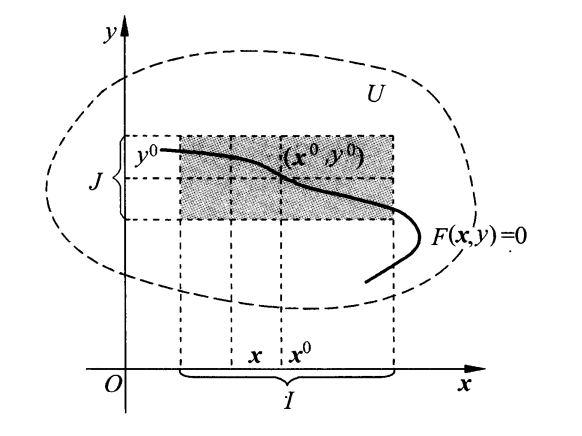
\includegraphics[width=0.5\textwidth]{img/ImplicitFunction.png}
    \caption{Implicit Function}
    \label{fig:ImplicitFunction}
\end{figure}

\begin{proof}
    Only the single-variable implicit function theorem is proved; 
    the multi-variable case can be derived using mathematical induction.
    
    Without loss of generality, assume \(F_y(x^0, y^0) > 0\).

    First, prove the \underline{existence of the implicit function}.  
    From the continuity of \(F_y(x^{0}, y^{0}) > 0\) and \(F_y(x, y)\), 
    it is known that there exist closed rectangle:
    \[
    D^* = \{(x, y) \mid |x - x_0| \leqslant \alpha, |y - y_0| \leqslant \beta\} \subset U,
    \]
    where the following holds:
    \[
    F_y(x, y) > 0.
    \]
    Thus, for fixed \(x_0\), the function \(F(x^{0}, y)\) is strictly monotonically increasing 
    within \([y^{0} - \beta, y^{0} + \beta]\). Furthermore, since:
    \[
    F(x^{0}, y^{0}) = 0,
    \]
    it follows that:
    \[
    F(x^{0}, y^{0} - \beta) < 0, \quad F(x^{0}, y^{0} + \beta) > 0.
    \]
    Due to the continuity of \(F(x, y)\) within \(D^*\), there exists \(\rho > 0\) such that along the line segment:
    \[
    x = x^{0} + \rho, \, y = y^{0} + \beta,
    \]
    we have \(F(x, y) > 0\), and along the line segment:
    \[
    x = x^{0} + \rho, \, y = y^{0} - \beta,
    \]
    we have \(F(x, y) < 0\).
    Therefore, for any point \(\bar{x} \in (x^{0} - \rho, x^{0} + \rho)\), treat \(F(x, y)\) as a single-variable function of \(y\). 
    Within \([y^{0} - \beta, y^{0} + \beta]\), this function is continuous. From the previous discussion, we know:
    \[
    F(\bar{x}, y^{0} - \beta) < 0, \quad F(\bar{x}, y^{0} + \beta) > 0.
    \]
    According to the zero point existence theorem~\ref{thm:Zero Point Existence Theorem}, 
    there must exist a unique \(\bar{y} \in [y^{0} - \beta, y^{0} + \beta]\) 
    such that \(F(\bar{x}, \bar{y}) = 0\). 
    Furthermore, because \(F_y(x, y) > 0\) within \(D^*\), this \(\bar{y}\) is unique.
    Denote the corresponding relationship as \(\bar{y} = f(\bar{x})\), 
    then the function \(y = f(x)\) is defined within \((x^{0} - \rho, x^{0} + \rho)\), 
    satisfying \(F(x, f(x)) = 0\), and clearly:
    \[
    y^{0} = f(x^{0}).
    \]

    Further proving \underline{the continuity of the implicit function} \(y = f(x)\) on \((x^{0} - \rho, x^{0} + \rho)\):  
    Let \(\bar{x} \in (x^{0} - \rho, x^{0} + \rho)\) be any point. 
    For any given \(\varepsilon > 0\) (\(\varepsilon\) being sufficiently small), 
    since \(F(\bar{x}, \bar{y}) = 0\) (\(\bar{y} = f(\bar{x})\)), from the previous discussion we know:  
    \[
    F(\bar{x}, \bar{y} - \varepsilon) < 0, \quad F(\bar{x}, \bar{y} + \varepsilon) > 0.
    \]
    Furthermore, due to the continuity of \(F(x, y)\) on \(D^*\), there exists \(\delta > 0\) such that:  
    \[
    F(x, \bar{y} - \varepsilon) < 0, \quad F(x, \bar{y} + \varepsilon) > 0, \quad \text{when} \quad x \in O(x^{0}, \delta).
    \]
    By reasoning similar to the previous discussion, 
    it can be obtained that when \(x \in O(x^{0}, \delta)\), 
    the corresponding implicit function value must satisfy \(f(x) \in (\bar{y} - \varepsilon, \bar{y} + \varepsilon)\), i.e.,  
    \[
    \left|f(x) - f(x^{0})\right| < \varepsilon.
    \]
    This implies that \(y = f(x)\) is continuous on \((x^{0} - \rho, x^{0} + \rho)\).  

    Finally, prove the \underline{differentiability} of \(y = f(x)\) on \((x^{0} - \rho, x^{0} + \rho)\):  
    Let \(\bar{x} \in (x^{0} - \rho, x^{0} + \rho)\) be any point. 
    Take \(\Delta x\) sufficiently small such that \(\bar{x} = x + \Delta x \in (x^{0} - \rho, x^{0} + \rho)\). 
    Denote \(\bar{y} = f(\bar{x})\) and \(\bar{y} + \Delta y = f(\bar{x})\). Clearly,  
    \[
    F(\bar{x}, \bar{y}) = 0 \quad \text{and} \quad F(\bar{x}, \bar{y} + \Delta y) = 0.
    \]
    Using the multi-variable function's mean value theorem~\ref{thm:Multi_Lagrange}, we obtain:  
    \begin{align*}
        0   &= F(\bar{x}, \bar{y} + \Delta y) - F(\bar{x}, \bar{y}) \\
            &= F_x(\bar{x} + \theta \Delta x, \bar{y} + \theta \Delta y) \Delta x + F_y(\bar{x} + \theta \Delta x, \bar{y} + \theta \Delta y) \Delta y,
    \end{align*}
    where \(0 < \theta < 1\).  
    Note that \(F_y \neq 0\) on \(D^*\), hence:  
    \[
    \frac{\Delta y}{\Delta x} = 
        -\frac{F_x(\bar{x} + \theta \Delta x, \bar{y} + \theta \Delta y)}{F_y(\bar{x} + \theta \Delta x, \bar{y} + \theta \Delta y)}.
    \]
    Let \(\Delta x \to 0\). Considering the continuity of \(F_x\) and \(F_y\), we obtain:  
    \[
    \frac{dy}{dx} \Big|_{x = \bar{x}} = -\frac{F_x(\bar{x}, \bar{y})}{F_y(\bar{x}, \bar{y})}.
    \]
    Thus:  
    \[
    f'(\bar{x}) = -\frac{F_x(\bar{x}, \bar{y})}{F_y(\bar{x}, \bar{y})}.
    \]

    The proof is complete.
\end{proof}

\begin{theorem}{Implicit Mapping Theorem}
    Let \( U \subset \mathbb{R}^{n+m} \) be an open set, and \( \mathbf{F}: U \to \mathbb{R}^m \) be a mapping. If:
    \begin{enumerate}
        \item \( \mathbf{F} \in C^k(U, \mathbb{R}^m) \), \( 1 \leqslant k \leqslant \infty \);
        \item \( \mathbf{F}(\mathbf{x}^0, \mathbf{y}^0) = 0 \), 
            where \( \mathbf{x}^0 = (x_1, x_2, \dots, x_n) \), \( \mathbf{y}^0 = (y_1, y_2, \dots, y_m) \), 
            \( (\mathbf{x}^0, \mathbf{y}^0) \in U \) 
            (implying \( \mathbf{F}(\mathbf{x}, \mathbf{y}) = \mathbf{0} \) 
            has a solution at \( (\mathbf{x}^0, \mathbf{y}^0) \));
        \item The determinant
        \[
        \det
        \begin{pmatrix}
            \frac{\partial F_1}{\partial y_1} & \cdots & \frac{\partial F_1}{\partial y_m} \\
            \vdots & \ddots & \vdots \\
            \frac{\partial F_m}{\partial y_1} & \cdots & \frac{\partial F_m}{\partial y_m}
        \end{pmatrix}_{(\mathbf{x}^0, \mathbf{y}^0)}
        = \det J_{\mathbf{y}} \mathbf{F}(\mathbf{x}^0, \mathbf{y}^0) \neq 0,
        \]
    \end{enumerate}
    then there exists an open neighborhood \( I \times J \subset U \subset \mathbb{R}^{n+m} \) 
    containing \( (\mathbf{x}^0, \mathbf{y}^0) \), such that:
    \begin{enumerate}
        \item For all \( \mathbf{x} \in I \), the system \( \mathbf{F}(\mathbf{x}, \mathbf{y}) = \mathbf{0} \) 
            has a unique solution \( \mathbf{y} = \mathbf{f}(\mathbf{x}) \), 
            where \( \mathbf{f}: I \to J \) is a mapping 
            (called \( \mathbf{f} \) the implicit function hidden in 
            \( \mathbf{F}(\mathbf{x}, \mathbf{f}(\mathbf{x})) = \mathbf{0} \));
        \item \( \mathbf{y}^0 = \mathbf{f}(\mathbf{x}^0) \);
        \item \( \mathbf{f} \in C^k(I, \mathbb{R}^m) \);
        \item For \( x \in I \),
        \[
        J_{\mathbf{f}}(x) = 
            - (J_{\mathbf{y}} \mathbf{F}(\mathbf{x}, \mathbf{f}(x)))^{-1} J_{\mathbf{x}} \mathbf{F}(\mathbf{x}, \mathbf{f}(x))
        = -
        \begin{pmatrix}
            \frac{\partial F_1}{\partial y_1} & \cdots & \frac{\partial F_1}{\partial y_m} \\
            \vdots & \ddots & \vdots \\
            \frac{\partial F_m}{\partial y_1} & \cdots & \frac{\partial F_m}{\partial y_m}
        \end{pmatrix}^{-1}
        \begin{pmatrix}
            \frac{\partial F_1}{\partial x_1} & \cdots & \frac{\partial F_1}{\partial x_n} \\
            \vdots & \ddots & \vdots \\
            \frac{\partial F_m}{\partial x_1} & \cdots & \frac{\partial F_m}{\partial x_n}
        \end{pmatrix},
        \]
    \end{enumerate}
    where \( \mathbf{y} = \mathbf{f}(\mathbf{x}) \).
\end{theorem}

\section{Applications of Multi-Variable Differential Calculus}
\begin{leftbarTitle}{Surface and Tangent Space}\end{leftbarTitle}
\begin{definition}{Parameterization of Surface}\label{def:Parameterization of Surface}
    Let \( \Delta \) be an open subset in \( \mathbb{R}^s \), 
    and \( \mathbf{x}: \Delta \to \mathbb{R}^n \) be a mapping, 
    where \( \mathbf{u} = (u_1, u_2, \dots, u_s) \to \mathbf{x}(\mathbf{u}) = 
    (x_1(u_1, u_2, \dots, u_s), x_2(u_1, u_2, \dots, u_s), \dots, x_n(u_1, u_2, \dots, u_s)) \). 
    Then \( M = \mathbf{x}(\Delta) = \{ \mathbf{x}(\mathbf{u}) \mid \mathbf{u} \in \Delta \} \) 
    is called an \( s \)-dimensional surface, and \( \mathbf{x}(\mathbf{u}) \) 
    is referred to as the parameterization of \( M \). 
    When \( \mathbf{x}(\mathbf{u}) \in C^k \) (\( k \geq 0 \)), 
    \( \mathbf{x} \) or \( M \) is called an \( s \)-dimensional \( C^k \) surface. 
    
    If \( \mathbf{x} \in C^k \) (\( k \geq 1 \)), \( \mathbf{x} \) or \( M \) 
    is called an \textbf{\( s \)-dimensional \( C^k \) smooth surface}. When
    \[
    \operatorname{rank}(x'_1(\mathbf{u}^0), x'_2(\mathbf{u}^0), \dots, x'_s(\mathbf{u}^0)) = 
    \operatorname{rank}
    \begin{pmatrix}
    \frac{\partial x_1}{\partial u_1} & \cdots & \frac{\partial x_1}{\partial u_s} \\
    \vdots & \ddots & \vdots \\
    \frac{\partial x_n}{\partial u_1} & \cdots & \frac{\partial x_n}{\partial u_s}
    \end{pmatrix}_{\mathbf{u}^0}
    = s,
    \]
    we call \( \mathbf{u}^0 \) or \( \mathbf{x}(\mathbf{u}^0) \) a \textbf{regular point} of the surface \( M \). 
    Otherwise, it is called a singular point. 
    Every point that is a regular point of the surface is referred to as an \textbf{\( s \)-dimensional \( C^k \) regular surface}. 
    At such points, \( \{x'_1, \dots, x'_s\} \) are linearly independent.
\end{definition}

When \( s = 1 \), \( t \) represents the parameter, a one-dimensional surface is commonly referred to as a curve. 
Considering a \( C^k \) (\( k \geq 1 \)) curve \( \mathbf{x}(t) \), we have:
\[
\mathbf{x}'(t) = \left( x_{1}'(t), x_{2}'(t), \cdots, x_{n}'(t) \right) .
\]
If \( t \) is a regular point, then 
\( \operatorname{rank}(\mathbf{x}'(t)) = \text{rank}(x'_1(t), x'_2(t), \dots, x'_n(t)) = 1 \); 
this is equivalent to \( \mathbf{x}'(t) \neq 0 \), which means \( x'_1(t), x'_2(t), \dots, x'_n(t) \) are not all zero.

We refer to \( \mathbf{x}'(t) \) as the tangent vector of the curve \( \mathbf{x}(t) \) at point \( t \). 
When \( t \) varies, a tangent vector field along the curve \( \mathbf{x}(t) \) is obtained. 
If \( \mathbf{x}(t) \) is a regular curve, 
\( \frac{\mathbf{x}'(t)}{\|\mathbf{x}'(t)\|} \) is the unit tangent vector field along the curve \( \mathbf{x}(t) \). 
It should be emphasized that \( \mathbf{x}'(t) \) or \( \frac{\mathbf{x}'(t)}{\|\mathbf{x}'(t)\|} \) 
always points outward from point \( t \).

\begin{definition}{Tangent Vector}
\end{definition}

\begin{leftbarTitle}{Unconditional Extremum}\end{leftbarTitle}

\begin{leftbarTitle}{Conditional Extremum}\end{leftbarTitle}


\chapter{Multiple Integrals}
\section{Multiple Integrals on Bounded Closed Regions}
\begin{leftbarTitle}{Definition of Multiple Integral}\end{leftbarTitle}

Initially, we define the double integral on a closed interval.
\begin{definition}{Double Integral on a Closed Interval}
    Let \( I = [a, b] \times [c, d] \) be a closed interval in \( \mathbb{R}^2 \), 
    (i.e., each boundary is parallel to the coordinate axes). Partition \( [a, b] \):
    \[
    T_x: a = x_0 < x_1 < \cdots < x_n = b.
    \]
    Partition \( [c, d] \):
    \[
    T_y: c = y_0 < y_1 < \cdots < y_m = d.
    \]
    Two sets of parallel lines \( x = x_i \, (i = 0, 1, \ldots, n) \) and \( y = y_j \, (j = 0, 1, \ldots, m) \) 
    divide \( I \) into \( n \times m \) subrectangles:
    \[
    [x_{i-1}, x_i] \times [y_{j-1}, y_j], \quad i = 1, \ldots, n, \, j = 1, \ldots, m.
    \]

    The union of these \( k \) subrectangles forms a partition \( T = T_x \times T_y = \{ I_1, I_2, \ldots, I_k \} \). 
    For each \( \xi^i \in I_i \, (i = 1, 2, \ldots, k) \), define the \textbf{Riemann sum} (also called a sum of integrals) as:
    \[
    \sum_{i=1}^k f(\boldsymbol{\xi}^i) v(I_i),
    \]
    where \( v(I_i) \) is the area of the rectangle \( I_i \), i.e., the product of its length and width. Denote:
    \[
    \lambda = \max(\text{diam}(I_1), \text{diam}(I_2), \ldots, \text{diam}(I_k)),
    \]
    where \( \text{diam}(I) \) is the diagonal length of the rectangle \( I \), 
    and \( \lambda \) is called the modulus or width of the partition \( T \). 
    The points 
    \( \boldsymbol{\xi} = (\boldsymbol{\xi}^1, \boldsymbol{\xi}^2, \ldots, \boldsymbol{\xi}^k) 
    \in I_1 \times I_2 \times \cdots \times I_k \) 
    are called sampling points for the Riemann sum.

    If there exists \( J \in \mathbb{R} \), such that \( \forall \varepsilon > 0 \), there exists \( \delta > 0 \), 
    such that when \( \lambda < \delta \), for all \( \boldsymbol{\xi} \in I_1 \times I_2 \times \cdots \times I_k \), we have:
    \[
    \left| \sum_{i=1}^k f(\boldsymbol{\xi}^i) v(I_i) - J \right| < \varepsilon,
    \]
    then \( f \) is said to be Riemann integrable on \( I \), and:
    \[
    J = \lim_{\lambda \to 0} \sum_{i=1}^k f(\boldsymbol{\xi}^i) v(I_i) =: 
    \iint_I f(x, y) \, \mathrm{d}x \mathrm{d}y \quad \text{or} \quad \int_I f \, \mathrm{d}v \quad \text{or} \quad \int_{I} f.
    \]

    The function \( f \) is said to have a double integral on \( I \), or simply \( f \) is integrable on \( I \). 
    Here \( f \) is called the integrand, \( I \) is called the integration region, 
    and \( \mathrm{d}v = \mathrm{d}x \mathrm{d}y \) is called the integration element.
\end{definition}

The defined double integral possesses properties similar to those of single-variable integrals.

On the basis of the above definition, we can extend it to the case of a bounded set.

\begin{definition}{Double Integral on a Bounded Set}
    Let \( \Omega \subset \mathbb{R}^2 \) be a bounded set, and \( f: \Omega \to \mathbb{R} \) a two-dimensional function. 
    Define:
    \[
    f_\Omega(\mathbf{x}) = f_\Omega(x, y) =
    \begin{cases} 
    f(x, y), & \text{if } \mathbf{x} = (x, y) \in \Omega, \\
    0, & \text{if } \mathbf{x} = (x, y) \not\in \Omega,
    \end{cases}
    \]
    and call this the \textbf{zero extension} of \( f \). 
    For any closed interval \( I \supset \Omega \), if \( f_\Omega \) is Riemann integrable on \( I \), 
    then \( f \) is said to be \textbf{Riemann integrable} on \( \Omega \) (abbreviated as integrable). 
    The integral of \( f \) on \( \Omega \), denoted as:
    \[
    \iint_\Omega f(x, y) \, \mathrm{d}x \mathrm{d}y = 
    \int_\Omega f \, \mathrm{dV} = \int_{\Omega} f = \int_{\Omega} f_\Omega = 
    \iint_I f_\Omega(x, y) \, \mathrm{d}x \mathrm{d}y,
    \]
    represents the Riemann integral of \( f \) on \( \Omega \).
\end{definition}

In above definition, the integral \( \int_\Omega f \) is independent of the choice of 
the closed interval \( I \) containing \( \Omega \) (this confirms the consistency of the definition).

It is worth noting that all the definitions and properties of double integrals 
can be extended to triple integrals and higher-dimensional integrals without excessive inconvenience.

\begin{leftbarTitle}{Necessary and Sufficient Conditions for Integrability}\end{leftbarTitle}

\begin{definition}{Set with Zero Area and Set with Zero Measure (Null Set)}
    Let \( A \subset \mathbb{R}^2 \). If for any \( \varepsilon > 0 \), 
    there exist \underline{finitely many} closed intervals \( I_1, I_2, \dots, I_k \) such that:
    \[
    \bigcup_{i=1}^k I_i \supset A, \quad \text{and} \quad \sum_{i=1}^k v(I_i) < \varepsilon,
    \]
    then \( A \) is called a \textbf{set with zero area}.

    Let \( A \subset \mathbb{R}^2 \). If for any \( \varepsilon > 0 \), 
    there exist at most \underline{countably many} closed intervals \( I_1, I_2, \dots, I_k, \dots \) such that:
    \[
    \bigcup_{i=1}^\infty I_i \supset A, \quad \text{and} \quad \sum_{i=1}^\infty v(I_i) < \varepsilon,
    \]
    then \( A \) is called a \textbf{set with zero measure (null set)}.
\end{definition}

\begin{definition}{Set with Finite Area}
    Let \( \Omega \subset \mathbb{R}^2 \) be a bounded set. 
    If the constant function \( 1 \) is integrable on \( \Omega \), 
    then \( \Omega \) is called a \textbf{set with finite area}, and the area of \( \Omega \) is defined as:
    \[
    v(\Omega) = \int_\Omega 1 = \iint_\Omega \mathrm{d}x \mathrm{d}y = \int_I 1_\Omega.
    \]

\end{definition}

Obviously, \(\Omega\) is a set with zero area if and only if \(\Omega\) has finite area, 
and \(v(\Omega) = \int_\Omega 1 = 0\).


\section{Properties and Calculation of Multiple Integrals}

\begin{leftbarTitle}{Reduction of Double Integral to Iterated Integral}\end{leftbarTitle}

\begin{theorem}{Reduction of Double Integral to Iterated Integral on a Closed Interval}\label{thm:Reduction of Double Integral to Iterated Integral on a Closed Interval}
    Let \( f \) be integrable on the closed interval \( I = [a, b] \times [c, d] \). 
    If \( \forall x \in [a, b] \), the function \( f(x, \cdot) \) is integrable on \( [c, d] \), then:
    \[
    \iint_I f = \int_a^b \left( \int_c^d f(x, y) \, \mathrm{d}y \right) \mathrm{d}x
    =: \int_{a}^{b}\mathrm{d}x\int_{c}^{d}f(x,y)\,\mathrm{d}y.
    \]

    Similarly, if \( \forall y \in [c, d] \), the function \( f(\cdot, y) \) is integrable on \( [a, b] \), then:
    \[
    \iint_I f = \int_c^d \left( \int_a^b f(x, y) \, \mathrm{d}x \right) \mathrm{d}y
    =: \int_{c}^{d}\mathrm{d}y\int_{a}^{b}f(x,y)\,\mathrm{d}x.
    \]
\end{theorem}

On the basis of the above theorem, we can extend it to the case of a bounded region.

\begin{theorem}{Reduction of Double Integral to Iterated Integral on a Bounded Set}
    Let \( \Omega \subset \mathbb{R}^2 \) be a set with infinite area, 
    and \( f: \Omega \to \mathbb{R} \) be bounded and continuous
    ~(\ref{fig:Double Integral on a Bounded Set}). 
    Denote the vertical projection of \( \Omega \) onto the \( x \)-axis as:
    \[
    I = \{ x \in \mathbb{R} \mid \exists y, \text{ s.t. } (x, y) \in \Omega \}.
    \]

    If \( \forall x \in I \), let \( \Omega_x = \{ y \in \mathbb{R} \mid (x, y) \in \Omega \} \) 
    be an interval (possibly reducing to a single point), then:
    \[
    \int_\Omega f = \int_I \mathrm{d}y \int_{\Omega_x} f(x, y) \, \mathrm{d}x.
    \]

    Similarly, denote the vertical projection of \( \Omega \) onto the \( y \)-axis as:
    \[
    J = \{ y \in \mathbb{R} \mid \exists x, \text{ s.t. } (x, y) \in \Omega \}.
    \]

    If \( \forall y \in J \), let \( \Omega_y = \{ x \in \mathbb{R} \mid (x, y) \in \Omega \} \) be an interval (possibly reducing to a single point), then:
    \[
    \int_\Omega f = \int_J \mathrm{d}y \int_{\Omega_y} f(x, y) \, \mathrm{d}x.
    \]
\end{theorem}
\begin{figure}[h]
    \centering
    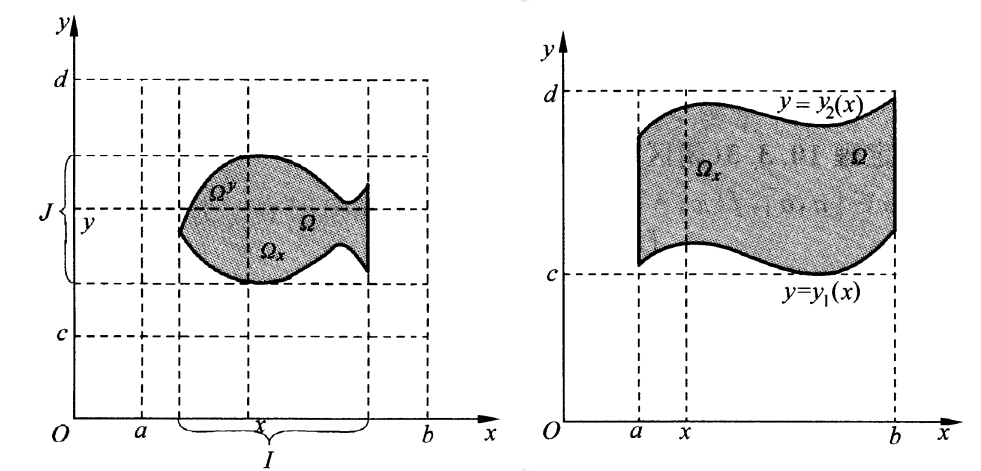
\includegraphics[width=0.5\textwidth]{img/IntegralImg.png}
    \caption{Double Integral on a Bounded Set}
    \label{fig:Double Integral on a Bounded Set}
\end{figure}

Specially, Let:
\[
\Omega = \{ (x, y) \in \mathbb{R}^2 \mid y_1(x) \leqslant y \leqslant y_2(x), \, a \leqslant x \leqslant b \},
\]
where the functions \( y_1 \) and \( y_2 \) are continuous on \( [a, b] \)~(\ref{fig:Double Integral on a Bounded Set}) 
and the function \( f \) is integrable on \( \Omega \). If \( \forall x \in [a, b] \), the single-variable integral:
\[
\int_{y_1(x)}^{y_2(x)} f(x, y) \, \mathrm{d}y
\]
exists, then:
\[
\int_\Omega f = \int_a^b \mathrm{d}x \int_{y_1(x)}^{y_2(x)} f(x, y) \, \mathrm{d}y.
\]
This area called the \textbf{type X region}, similarly, we can define the \textbf{type Y region}.


According to~\ref{thm:Reduction of Double Integral to Iterated Integral on a Closed Interval},
we can derive the formula of multiplicative property for double integral.

\begin{theorem}{Formula of Multiplicative Property for Double Integral}
    Let \( f \in C([a, b]) \), \( g \in C([c, d]) \). 
    Then the function \( h(x, y) = f(x) g(y) \) is integrable on the closed interval \( I = [a, b] \times [c, d] \), 
    and:
    \[
    \iint_I h(x, y) \, \mathrm{d}x \mathrm{d}y = \left( \int_a^b f(x) \, \mathrm{d}x \right) 
    \left( \int_c^d g(y) \, \mathrm{d}y \right).
    \]
\end{theorem}

\begin{example}
    Let \(p(x)\in R[a,b],p(x)>0,x\in [a,b]\), the monotonicity of \(f(x), g(x)\) is same,
    prove that
    \[
    \int_{a}^{b}p(x)f(x)\mathrm{d}x \int_{a}^{b}p(x)g(x)\mathrm{d}x
    \leqslant  \int_{a}^{b}p(x)\mathrm{d}x \int_{a}^{b}p(x)f(x)g(x)\mathrm{d}x
    \]
\end{example}
\begin{proof}
    Let
    \[
    I = \int_{a}^{b}p(x)\mathrm{d}x \int_{a}^{b}p(x)f(x)g(x)\mathrm{d}x
        - \int_{a}^{b}p(x)f(x)\mathrm{d}x \int_{a}^{b}p(x)g(x)\mathrm{d}x,
    \]
    then
    \[
    I = \int_{a}^{b}\int_{a}^{b}p(x)p(y)g(y)(f(x)-f(y))\mathrm{d}x\mathrm{d}y,
    \]
    similarly,
    \[
    I = \int_{a}^{b}\int_{a}^{b}p(x)p(y)g(x)(f(x)-f(y))\mathrm{d}x\mathrm{d}y.
    \]
    Then 
    \[
    2I = \int_{a}^{b}\int_{a}^{b}p(x)p(y)(g(y)-g(x))(f(x)-f(y))\mathrm{d}x\mathrm{d}y \geqslant  0,
    \]
    which implies
    \[
    I \geqslant  0.
    \]
    The proof is complete.
\end{proof}

\begin{leftbarTitle}{Calculation of Triple Integrals}\end{leftbarTitle}
\begin{example}\label{eg:Triple Integral of Cone}
    Calculating \(I = \iiint_{ \Omega }z^{2}\mathrm{d}x\mathrm{d}y\mathrm{d}z\),
    where \(\Omega\) is the cone defined by \(z^{2} = \frac{h^{2}}{R^{2}}(x^{2}+y^{2})\) 
    and \(z = h\)~(\ref{fig:Cone}).
    \begin{figure}[h]
        \centering
        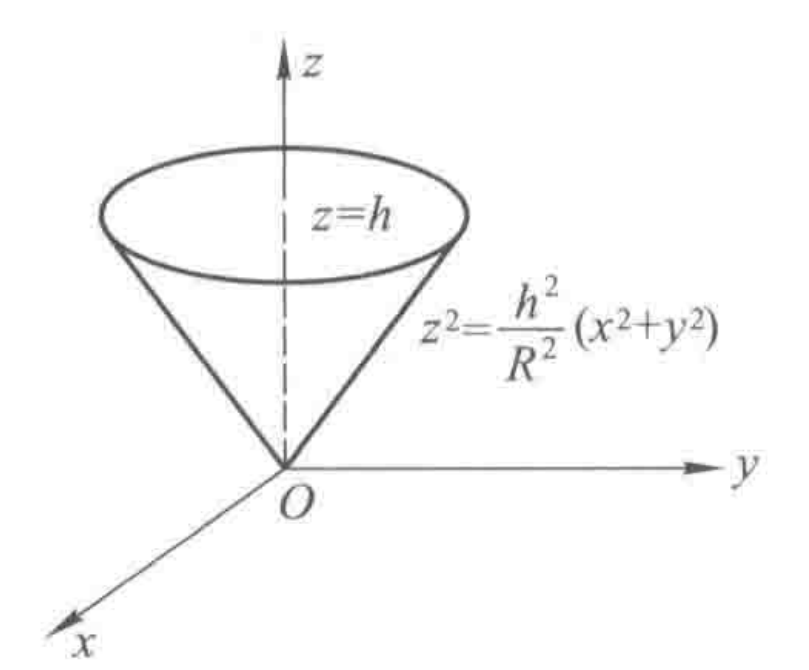
\includegraphics[width=0.4\textwidth]{img/cone.png}
        \caption{Cone Example.}
        \label{fig:Cone}
    \end{figure}
\end{example}

\begin{example}\label{eg:Project Method Example}
    Calculating \(I = \iiint_{ \Omega }xy\mathrm{d}x\mathrm{d}y\mathrm{d}z\),
    where \(\Omega\) is the region defined 
    by \(0 \leqslant z \leqslant xy, 0\leqslant y \leqslant 1-x, 0\leqslant x \leqslant 1\)
    ~(\ref{fig:Project Method Example}).
    \begin{figure}[h]
        \centering
        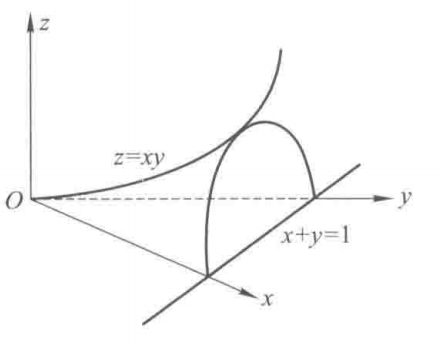
\includegraphics[width=0.4\textwidth]{img/project_method_example.png}
        \caption{Project Method Example.}
        \label{fig:Project Method Example}
    \end{figure}
\end{example}

\vspace{1cm}
With the help of examples above, we can derive \textbf{two methods for calculating triple integrals}.

\begin{description}
\item[First 2 then 1 (Section Method)] 
Fix one variable (e.g., \(z\)), first perform a double integral over the other two variables (e.g., \(x,y\)) 
on the "section region" corresponding to the fixed variable, 
and then perform a definite integral over the fixed variable (\(z\)) within its range of values.

This method is convenient when the area of the section region is easy to calculate, 
or when the integrand is only related to the "later-integrated variable" (e.g., only related to \(z\)).

In the example~\ref{eg:Triple Integral of Cone}, the following steps are taken:
\begin{enumerate}
    \item Determine the range of z: \(z \in [0, h]\). 
    \item Determine the section region \(D_z\): 
        For a fixed \(z\), \(D_z\) is the region on the \(xy\)-plane satisfying \(\frac{h^2}{R^2}(x^2 + y^2) \leqslant z^2\), 
        which is a circle with radius \(\frac{R}{h}z\).
    \item Split the integral: 
        \[
        I = \int_{0}^{h} \left( \iint_{D_z} z^2 \,\mathrm{d}x\mathrm{d}y \right) \,\mathrm{d}z.
        \] 
        Since \(z^2\) is independent of \(x\) and \(y\), it can be factored out:
        \(I = \int_{0}^{h} z^2 \left( \iint_{D_z} \,\mathrm{d}x\mathrm{d}y \right) dz\).
    \item Calculate the double integral (area of the section): 
        \[
        \iint_{D_z} \,\mathrm{d}x\mathrm{d}y = \pi \left( \frac{R}{h}z \right)^2 = \pi \frac{R^2}{h^2} z^{2}.
        \]
    \item Calculate the definite integral: 
        \[
        I = \int_{0}^{h} z^2 \cdot \pi \frac{R^2}{h^2} z^2 \,\mathrm{d}z = \frac{\pi R^2 h^3}{5}.\
        \]
\end{enumerate}

\item[First 1 then 2 (Project Method)]
Fix two variables (e.g., \(x,y\)), first perform a definite integral over the third variable (e.g., \(z\)) 
on the "vertical line segment" corresponding to the fixed variables, 
and then perform a double integral over the fixed two variables ( \(x,y\)) on their "projection region. 

This method is convenient when the projection region of the integral region on 
a certain coordinate plane (e.g., \(xy\)-plane) is easy to determine, 
and the upper and lower limits of a single variable (e.g., \(z\)) can 
be easily expressed by the other two variables.

In the example~\ref{eg:Project Method Example}, the following steps are taken:
\begin{enumerate}
    \item Determine the projection region \(D_{xy}\):\(D_{xy}\) is the region on the \(xy\)-plane 
        bounded by \(x + y \leqslant 1\), \(x \geq 0\), and \(y \geq 0\), 
        which can be expressed as \(0 \leqslant x \leqslant 1\) and \(0 \leqslant y \leqslant 1 - x\).
    \item Determine the range of \(z\): \(z \in [0, xy]\) (since \(z\) is bounded below by \(z = 0\) and above by \(z = xy\)).
    \item Split the integral: 
        \[
        I = \iint_{D_{xy}}\, \left( \int_{0}^{xy} xy \mathrm{d}z \right)  \mathrm{d}x \mathrm{d}y,
        \]
        split the double integral on \(D_{xy}\) as:
        \(I = \int_{0}^{1} \, \mathrm{d}x \int_{0}^{1 - x} \, \mathrm{d}y  \int_{0}^{xy} xy \, \mathrm{d}z\).
        (Since \(xy\) is independent of \(z\), it can be factored out without affecting the integral:
        \(I = \int_{0}^{1} \, \mathrm{d}x \int_{0}^{1 - x} xy \, \mathrm{d}y  \int_{0}^{xy} \, \mathrm{d}z\).)
    \item Calculate the inner integral (with respect to \(z\)):
        \(\int_{0}^{xy} xy \, dz = xy \cdot \int_{0}^{xy} dz 
        = xy \cdot \left. z \right|_{0}^{xy} = xy \cdot xy = x^2 y^2\).
    \item Calculate the middle integral (with respect to \(y\)):
        Substitute the result of the inner integral,
        \[
        \int_{0}^{1 - x} x^2 y^2 \, dy 
        = x^2 \cdot \left. \frac{y^3}{3} \right|_{0}^{1 - x} = \frac{x^2 (1 - x)^3}{3}.
        \]
    \item Calculate the outer integral (with respect to \(x\)):Substitute the result of the middle integral:
        \begin{align*}
            \int_{0}^{1} \frac{x^2 (1 - x)^3}{3} \, dx &= \frac{1}{3} \int_{0}^{1} (x^2 - 3x^3 + 3x^4 - x^5) \, dx \\
            &= \frac{1}{3} \left( \left. \frac{x^3}{3} - \frac{3x^4}{4} + \frac{3x^5}{5} - \frac{x^6}{6} \right|_{0}^{1} \right) \\
            &= \frac{1}{3} \left( \frac{1}{3} - \frac{3}{4} + \frac{3}{5} - \frac{1}{6} \right) \\
            &= \frac{1}{180}.
        \end{align*}
\end{enumerate}
\end{description}
% 选择哪种方法的技巧
Some tips for choosing between the two methods (take the above two examples as reference):

\begin{tabular}{p{0.45\textwidth} p{0.45\textwidth}}
    \textbf{First 2 then 1 (Section Method)} & \textbf{First 1 then 2 (Project Method)} \\
    \toprule
    Section area \(D_{z}\) is easy to calculate & Projection region \(D_{xy}\) is easy to determine \\
    \hline
    Integrand is only related to \(z\) & Upper and lower limits \(z\) can be easily expressed by the other two variables \(x,y\) \\
    \bottomrule
\end{tabular}



\section{Variable Substitution in Multiple Integrals}
\begin{theorem}{Variable Substitution in Double Integral}
    Let \( \Omega \subset \mathbb{R}^2 \) be an open set, and let the mapping:
    \[
    \mathbf{F}: \Omega \to \mathbb{R}^2, \quad (u, v) \mapsto \mathbf{F}(u, v) = (x(u, v), y(u, v))
    \]
    satisfy the following conditions:
    \begin{enumerate}
        \item \( \mathbf{F} \in C^1(\Omega, \mathbb{R}^2) \);
        \item \( \frac{\partial (x, y)}{\partial (u, v)} 
            = \det J\mathbf{F}(u, v) = \det J\mathbf{F}(\mathbf{p}) \neq 0, \quad \mathbf{p} = (u, v) \in \Omega \);
        \item \( \mathbf{F} \) is injective.
    \end{enumerate}

    If the set \( \Delta \) is a set with finite area and 
    \( \overline{\Delta} \subset \Omega \), and \( f \) is continuous on \( \mathbf{F}(\Omega) \), 
    then \( \mathbf{F}(\Delta) \) is also a set with finite area, and:
    \[
    \iint_{\mathbf{F}(\Delta)} f = \iint_{\Delta} f \circ \mathbf{F} \left| \det J\mathbf{F} \right|,
    \]
    i.e.,
    \[
    \iint_{F(\Delta)} f(x, y) \, \mathrm{d}x \mathrm{d}y = 
    \iint_{\Delta} f(x(u, v), y(u, v)) \left| \frac{\partial (x, y)}{\partial (u, v)} \right| \, \mathrm{d}u \mathrm{d}v.
    \]
\end{theorem}

For triple and higher-dimensional integrals, the variable substitution theorem is similar to the above theorem.

\vspace{0.7cm}
Some common variable substitutions in multiple integrals are as follows:
\begin{description}
\item[Polar Coordinates]
\[
\begin{cases} 
    x = r \cos \theta, \\ 
    y = r \sin \theta,
\end{cases}
\qquad
\begin{cases} 
    r = \sqrt{x^2 + y^2},\quad r\geqslant 0 \\ 
    \theta = \arctan\left(\frac{y}{x}\right)\quad x\neq 0, \theta\in [0, 2\pi].
\end{cases}
\]
and
\[
\frac{\partial (x,y)}{\partial (r,\theta)} = r.
\]

\item[Cylindrical Coordinate System]
\[
\begin{cases} 
    x = r \cos \theta, \\ 
    y = r \sin \theta, \\
    z = z,
\end{cases}
\qquad
\begin{cases} 
    r = \sqrt{x^2 + y^2},\quad r\geqslant 0 \\ 
    \theta = \arctan\left(\frac{y}{x}\right)\quad x\neq 0, \theta\in [0, 2\pi], \\
    z = z.
\end{cases}
\]
and
\[
\frac{\partial (x,y,z)}{\partial (r,\theta,\varphi)} = r.
\]

\item[Spherical Coordinate System]
\[
\begin{cases} 
    x = r \sin \varphi \cos \theta, \\ 
    y = r \sin \varphi \sin \theta, \\
    z = r \cos \varphi,
\end{cases}
\qquad
\begin{cases} 
    r = \sqrt{x^2 + y^2 + z^2},\quad r\geqslant 0 \\ 
    \varphi = \arccos\left(\frac{z}{r}\right)\quad r\neq 0, \varphi\in [0, \pi], \\
    \theta = \arctan\left(\frac{y}{x}\right)\quad x\neq 0, \theta\in [0, 2\pi].
\end{cases}
\]
and
\[
\frac{\partial (x,y,z)}{\partial (r,\theta,\varphi)} = r^2 \sin \varphi.
\]

\end{description}
\begin{figure}[h]
    \centering
    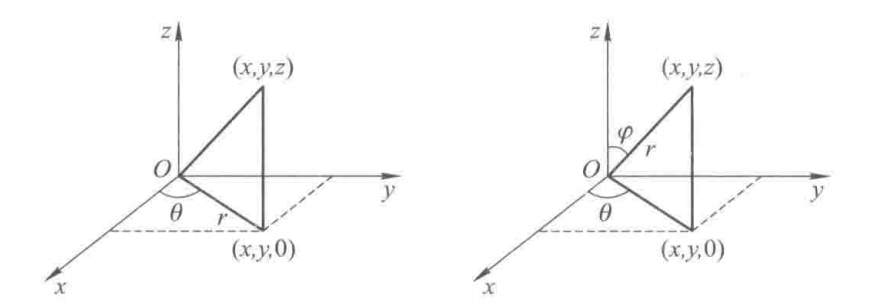
\includegraphics[width=0.8\textwidth]{img/coordinate.png}
    \caption{Cylindrical and Spherical Coordinate Systems}
\end{figure}




\section{Improper Multiple Integrals}


\chapter{Line Integrals and Surface Integrals}
\section{Line Integrals and Surface Integrals of scalar fields}
\begin{leftbarTitle}{Line Integral of Scalar Field}\end{leftbarTitle}
\begin{definition}{Line Integral of Scalar Field}
    Let \(L\) is a rectifiable continuous curve in \(\mathbb{R}^3\), whose endpoints are \(A\) and \(B\),
    and \(f(x, y, z)\) is bounded on \(L\).
    Partition \(L\) into \(n\) segments by points \(A = P_0, P_1, \ldots, P_n = B\),
    and select a point \(\boldsymbol{\xi}_{i}\) on each segment \(P_{i-1}P_i\) (\(i = 1, 2, \ldots, n\)).
    Remark that the length of segment \(P_{i-1}P_i\) is \(\Delta s_i\) (\(i=1,2,\cdots n\)),
    and make the sum:
    \[
    \sum_{i=1}^{n} f(\boldsymbol{\xi}_i) \Delta s_i.
    \]
    If when \( \lambda \) (the length of the longest segment) tends to \(0\),
    the above sum tends to a limit \(I\) independent of the partition and the choice of points \(\boldsymbol{\xi}_i\),
    then \(I\) is called the \textbf{line integral of the scalar field \(f\) along the curve \(L\)},
    denoted as:
    \[
    \int_{L} f \, \mathrm{d}s.
    \]
    That is,
    \[
    I = \int_{L} f(\boldsymbol{\xi}) \, \mathrm{d}s =
    \lim_{\lambda \to 0} \sum_{i=1}^{n} f(\boldsymbol{\xi}_i) \Delta s_i.
    \]
\end{definition}

\begin{theorem}
    Let \(L\) be a \(C^{1}\) smooth regular curve parameterized by \(\mathbf{x}(t) = (x(t), y(t), z(t)), t \in [\alpha, \beta]\),
    and \(f\) be continuous on \(L\).
    Then:
    \[
    \int_{L} f \, \mathrm{d}s = \int_{\alpha}^{\beta} f(\mathbf{x}(t)) \|\mathbf{x}'(t)\| \, \mathrm{d}t.
    = \int_{\alpha}^{\beta} f(x(t), y(t), z(t)) \sqrt{(x'(t))^2 + (y'(t))^2 + (z'(t))^2} \, \mathrm{d}t.
    \]
\end{theorem}

\begin{leftbarTitle}{Surface Theory}\end{leftbarTitle}

\begin{leftbarTitle}{Surface Integrals of Scalar Fields}\end{leftbarTitle}
\begin{definition}{Surface Integral of Scalar Field}
    Let \(\Sigma\) be a piecewise smooth surface in \(\mathbb{R}^3\),
    and \(f(x, y, z)\) be bounded on \(\Sigma\).
    Partition \(\Sigma\) into \(n\) small pieces \(\Delta\Sigma_1, \Delta\Sigma_2, \ldots, \Delta\Sigma_n\)
    with smooth curve webs,
    and select a point \(\boldsymbol{\xi}_i\) on each piece \(\Delta\Sigma_i\) (\(i = 1, 2, \ldots, n\)).
    Remark that the area of piece \(\Delta\Sigma_i\) is \(\Delta S_i\) (\(i=1,2,\cdots n\)),
    and make the sum:
    \[
    \sum_{i=1}^{n} f(\boldsymbol{\xi}_i) \Delta S_i.
    \]
    If when \( \lambda \) (the area of the largest piece) tends to \(0\),
    the above sum tends to a limit \(I\) independent of the partition and the choice of points \(\boldsymbol{\xi}_i\),
    then \(I\) is called the \textbf{surface integral of the scalar field \(f\) over the surface \(\Sigma\)},
    denoted as:
    \[
    \iint_{\Sigma} f \, \mathrm{d}S.
    \]
    That is,
    \[
    I = \iint_{\Sigma} f(\boldsymbol{\xi}) \, \mathrm{d}S =
    \lim_{\lambda \to 0} \sum_{i=1}^{n} f(\boldsymbol{\xi}_i) \Delta S_i.
    \]
\end{definition}

\begin{theorem}
    Let \(\Sigma\) be a piecewise smooth closed surface parameterized by 
    \(\mathbf{r}(u, v) = (x(u, v), y(u, v), z(u, v)), (u, v) \in D\),
    and \(f\) be continuous on \(\Sigma\).
    \(x, y, z\) have continuous first-order partial derivatives with respect to \(u\) and \(v\) on \(D\),
    and according Jacobian matrix 
    \[
    J = \begin{pmatrix}
        \frac{\partial x}{\partial u} & \frac{\partial x}{\partial v} \\
        \frac{\partial y}{\partial u} & \frac{\partial y}{\partial v} \\
        \frac{\partial z}{\partial u} & \frac{\partial z}{\partial v}
    \end{pmatrix}
    \]
    is of full rank.
    Then:
    \[
    \iint_{\Sigma} f \, \mathrm{d}S = \iint_{D} f(\mathbf{r}(u, v)) 
    \left\| \frac{\partial \mathbf{r}}{\partial u} \times \frac{\partial \mathbf{r}}{\partial v} \right\| \, \mathrm{d}u \mathrm{d}v
    = \iint_{D} f(x(u, v), y(u, v), z(u, v)) 
    \sqrt{EG-F^{2}} \, \mathrm{d}u \mathrm{d}v,
    \]
    where
    \begin{align*}
        &E = \mathbf{r}_{u} \cdot \mathbf{r}_{u} = x_{u}^2 + y_{u}^2 + z_{u}^2, \\        
        &F = \mathbf{r}_{u} \cdot \mathbf{r}_{v} = x_{u} x_{v} + y_{u} y_{v} + z_{u} z_{v}, \\
        &G = \mathbf{r}_{v} \cdot \mathbf{r}_{v} = x_{v}^2 + y_{v}^2 + z_{v}^2,
    \end{align*}
    and it is called the Gauß coefficients of the surface \(\Sigma\).
\end{theorem}

\section{Differential Form and Exterior Differentiation}
Let \(\mathrm{d}x_{i}, \mathrm{d}x_{j}\) be differentials of independent variables \(x_{i}, x_{j}\).

In \(\mathbb{R}^{1}\):
\begin{align*}
    &\text{0-form: } f(x), \\
    &\text{1-form: } \omega = f(x)\mathrm{d}x, \\
    &\text{k-form (\(k\geqslant 2\)): } \omega = \sum_{1 \leqslant i_{1} < i_{2} < \cdots < i_{k} \leqslant n}
        f_{i_{1} i_{2} \cdots i_{k}}(x_{1}, x_{2}, \cdots, x_{n})
        \mathrm{d}x_{i_{1}} \wedge \mathrm{d}x_{i_{2}} \wedge \cdots \wedge \mathrm{d}x_{i_{k}} = 0.
\end{align*}

In \(\mathbb{R}^{2}\):
\begin{align*}
    &\text{0-form: } f(x, y), \\
    &\text{1-form: } \omega = P(x, y)\mathrm{d}x + Q(x, y)\mathrm{d}y, \\
    &\text{2-form: } \omega = f(x, y)\mathrm{d}x \wedge \mathrm{d}y, \\
    &\text{k-form (\(k\geqslant 3\)): } \omega = \sum_{1 \leqslant i_{1} < i_{2} < \cdots < i_{k} \leqslant n}
        f_{i_{1} i_{2} \cdots i_{k}}(x_{1}, x_{2}, \cdots, x_{n})
        \mathrm{d}x_{i_{1}} \wedge \mathrm{d}x_{i_{2}} \wedge \cdots \wedge \mathrm{d}x_{i_{k}} = 0.
\end{align*}

In \(\mathbb{R}^{3}\):
\begin{align*}
    &\text{0-form: } f(x, y, z), \\
    &\text{1-form: } \omega = P(x, y, z)\mathrm{d}x + Q(x, y, z)\mathrm{d}y + R(x, y, z)\mathrm{d}z, \\
    &\text{2-form: } \omega = P(x, y, z)\mathrm{d}y \wedge \mathrm{d}z + Q(x, y, z)\mathrm{d}z \wedge \mathrm{d}x + R(x, y, z)\mathrm{d}x \wedge \mathrm{d}y, \\
    &\text{3-form: } \omega = f(x, y, z)\mathrm{d}x \wedge \mathrm{d}y \wedge \mathrm{d}z, \\
    &\text{k-form (\(k\geqslant 4\)): } \omega = \sum_{1 \leqslant i_{1} < i_{2} < \cdots < i_{k} \leqslant n}
        f_{i_{1} i_{2} \cdots i_{k}}(x_{1}, x_{2}, \cdots, x_{n})
        \mathrm{d}x_{i_{1}} \wedge \mathrm{d}x_{i_{2}} \wedge \cdots \wedge \mathrm{d}x_{i_{k}} = 0.
\end{align*}

Here, \(\wedge\) is called the \textbf{wedge product}, which satisfies:
\begin{enumerate}
    \item Skew symmetric: \(\mathrm{d}x_{i} \wedge \mathrm{d}x_{j} = -\mathrm{d}x_{j} \wedge \mathrm{d}x_{i}\), 
    \item Associative: \((\mathrm{d}x_{i} \wedge \mathrm{d}x_{j}) \wedge \mathrm{d}x_{k} = \mathrm{d}x_{i} \wedge (\mathrm{d}x_{j} \wedge \mathrm{d}x_{k})\),
    \item In a fixed dimension, the wedge product of k-forms becomes zero (as higher forms are not defined), 
        for example, in \(3\)-dimensional space, a \(4\)-form is equal to \(0\).
\end{enumerate}
\textbf{Differential form} is a skew symmetric tensor on vector field.


\begin{definition}{Exterior Differentiation}
    Let \(\omega\) be a \(k\)-form on \(\mathbb{R}^{n}\),
    \[
    \omega = \sum_{1 \leqslant i_{1} < i_{2} < \cdots < i_{k} \leqslant n}
        f_{i_{1} i_{2} \cdots i_{k}}(x_{1}, x_{2}, \cdots, x_{n})
        \mathrm{d}x_{i_{1}} \wedge \mathrm{d}x_{i_{2}} \wedge \cdots \wedge \mathrm{d}x_{i_{k}},
    \]
    where \(f_{i_{1} i_{2} \cdots i_{k}}\) are functions with continuous first-order partial derivatives.
    The exterior differentiation of \(\omega\) is defined as:
    \[
    \mathrm{d}\omega = \sum_{1 \leqslant i_{1} < i_{2} < \cdots < i_{k} \leqslant n}
        \mathrm{d}f_{i_{1} i_{2} \cdots i_{k}}(x_{1}, x_{2}, \cdots, x_{n})
        \wedge \mathrm{d}x_{i_{1}} \wedge \mathrm{d}x_{i_{2}} \wedge \cdots \wedge \mathrm{d}x_{i_{k}},
    \]
    where
    \[
    \mathrm{d}f = \frac{\partial f}{\partial x_1}\mathrm{d}x_1 + 
    \frac{\partial f}{\partial x_2}\mathrm{d}x_2 + 
    \cdots + 
    \frac{\partial f}{\partial x_n}\mathrm{d}x_n.
    \]
    Note that the exterior differentiation of a \(k\)-form is a \(k+1\)-form.
\end{definition}
\begin{property}
    \begin{description}
        \item[Linearity] \(\mathrm{d}(\alpha \omega+ \beta \eta) = \alpha \mathrm{d}\omega + \beta \mathrm{d}\eta\),
        where \(\alpha, \beta\) are constants.
        \item[Leibniz Rule] \(\mathrm{d}(\omega \wedge \eta) = \mathrm{d}\omega \wedge \eta + (-1)^{k} \omega \wedge \mathrm{d}\eta\),
        where \(\omega\) is a \(k\)-form.
        \item[Nilpotency] \(\mathrm{d}(\mathrm{d}\omega) = 0\).
    \end{description}
\end{property}


\section{Orientation of Curves and Surfaces}

\section{Line Integrals and Surface Integrals of Vector Fields}
\begin{leftbarTitle}{Line Integral of Vector Field}\end{leftbarTitle}
\begin{definition}{Line Integral of Vector Field}
    Let \(\overset{\rightharpoonup}{L}\) be a orientated smooth curve in \(\mathbb{R}^3\),
    whose endpoints are \(A\) and \(B\).
    Take unit tangent vector \(\boldsymbol{\tau}=(\cos\alpha, \cos\beta, \cos\gamma)\) 
    at each point of \(\overset{\rightharpoonup}{L}\), making it consistent with the orientation of \(\overset{\rightharpoonup}{L}\).
    Let \(\mathbf{f}(x, y, z) = P(x, y, z)\mathbf{i} + Q(x, y, z)\mathbf{j} + R(x, y, z)\mathbf{k}\) 
    be a vector-valued function on \(\overset{\rightharpoonup}{L}\), then 
    \[
    \int_{\overset{\rightharpoonup}{L}} \mathbf{f} \cdot \boldsymbol{\tau} \mathrm{d}\mathbf{s} =
    \int_{\overset{\rightharpoonup}{L}} \left[P \cos\alpha + Q \cos\beta + R \cos\gamma\right] \, \mathrm{d}s
    \]
    is called the \textbf{line integral of the vector field \(\mathbf{f}\) along the oriented curve \(\overset{\rightharpoonup}{L}\)}
    (if the right-hand side exists).
\end{definition}
Consider a differential arc length element \( \mathrm{d}s \) at a point \((x, y, z)\) on the curve \( L \). 
We form the vector \( \mathrm{d}\mathbf{s} = \boldsymbol{\tau} \mathrm{d}s \), 
where \( \boldsymbol{\tau} = (\cos\alpha, \cos\beta, \cos\gamma) \) represents 
the unit tangent vector of curve \( L \) at \((x, y, z)\), pointing along the direction of \( L \). 
The projection of \( \mathrm{d}s \) onto the \( x \)-axis is given by \(\cos\alpha \, \mathrm{d}s\). 
Therefore, we denote:
\[
\mathrm{d}x = \cos\alpha \, \mathrm{d}s, \quad \mathrm{d}y = \cos\beta \, \mathrm{d}s, \quad 
\mathrm{d}z = \cos\gamma \, \mathrm{d}s.
\]
Thus, the second type of line integral can be expressed as:
\[
\int_{\overset{\rightharpoonup}{L}} \mathbf{f} \cdot \boldsymbol{\tau} \mathrm{d}s = \int_{\overset{\rightharpoonup}{L}} \mathbf{f} \, \mathrm{d} \mathbf{s} 
= \int_{\overset{\rightharpoonup}{L}} P(x, y, z) \mathrm{d}x + Q(x, y, z) \mathrm{d}y + R(x, y, z) \mathrm{d}z.
\]
This line integral is also referred to as the integral of the \(1\)-form:
\[
\omega = P(x, y, z) \mathrm{d}x + Q(x, y, z) \mathrm{d}y + R(x, y, z) \mathrm{d}z.
\]
The second type of line integral of \( \omega \) along the curve \( L \) is denoted as:
\[
\int_{\overset{\rightharpoonup}{L}} \omega.
\]

\begin{theorem}
    Let \(\overset{\rightharpoonup}{L}\) be a \(C^{1}\) smooth regular oriented curve parameterized by 
    \(\mathbf{x}(t) = (x(t), y(t), z(t)), t \in [\alpha, \beta]\),
    and \(\mathbf{f} = P\mathbf{i} + Q\mathbf{j} + R\mathbf{k}\) be continuous on \(\overset{\rightharpoonup}{L}\).
    Then:
    \begin{gather*}
    \int_{\overset{\rightharpoonup}{L}} \mathbf{f} \cdot \boldsymbol{\tau} \mathrm{d}s =
    \int_{\alpha}^{\beta} \mathbf{f}(\mathbf{x}(t)) \cdot \mathbf{x}'(t) \, \mathrm{d}t \\
    = \int_{\alpha}^{\beta} [P(x(t), y(t), z(t)) x'(t) + Q(x(t), y(t), z(t)) y'(t) + R(x(t), y(t), z(t)) z'(t)] \, \mathrm{d}t.
    \end{gather*}
\end{theorem}
\begin{leftbarTitle}{Surface Integral of Vector Field}\end{leftbarTitle}
\begin{definition}{Surface Integral of Vector Field}
    Let \(\overset{\rightharpoonup}{\Sigma}\) be an orientated smooth surface in \(\mathbb{R}^3\),
    and \(\mathbf{f}(x, y, z) = P(x, y, z)\mathbf{i} + Q(x, y, z)\mathbf{j} + R(x, y, z)\mathbf{k}\) 
    be a vector-valued function on \(\overset{\rightharpoonup}{\Sigma}\).
    Each point appoints a unit normal vector \(\mathbf{n}=(\cos\alpha, \cos\beta, \cos\gamma)\).
    Then 
    \[
    \iint_{\overset{\rightharpoonup}{\Sigma}} \mathbf{f} \cdot \mathbf{n} \mathrm{d}S =
    \iint_{\overset{\rightharpoonup}{\Sigma}} \left[P \cos\alpha + Q \cos\beta + R \cos\gamma\right] \, \mathrm{d}S
    \]
    is called the \textbf{surface integral of the vector field \(\mathbf{f}\) over the oriented surface \(\overset{\rightharpoonup}{\Sigma}\)}
    (if the right-hand side exists).
\end{definition}
Consider a differential area element \( \mathrm{d}S \) at a point \((x, y, z)\) on the surface \( \Sigma \). 
We form the vector \( \mathrm{d}\mathbf{S} = \mathbf{n} \mathrm{d}S \), 
where \( \mathbf{n} = (\cos\alpha, \cos\beta, \cos\gamma) \) represents
the unit normal vector of surface \( \Sigma \) at \((x, y, z)\),
pointing along the orientation of \( \Sigma \).
The projection of \( \mathrm{d}S \) onto the \( x \)-axis is given by \(\cos\alpha \, \mathbf{\mathrm{d}}S\). 
Therefore, we denote:
\[
\mathrm{d}y \wedge \mathrm{d}z = \cos\alpha \, \mathrm{d}S, \quad \mathrm{d}z \wedge \mathrm{d}x = \cos\beta \, \mathrm{d}S, \quad 
\mathrm{d}x \wedge \mathrm{d}y = \cos\gamma \, \mathrm{d}S.
\]
Thus, the surface integral can be expressed as:
\[
\iint_{\overset{\rightharpoonup}{\Sigma}} \mathbf{f} \cdot \mathbf{n} \mathrm{d}S = 
\iint_{\overset{\rightharpoonup}{\Sigma}} P \mathrm{d}y \wedge \mathrm{d}z + Q \mathrm{d}z \wedge \mathrm{d}x + R \mathrm{d}x \wedge \mathrm{d}y
= \iint_{\Sigma} P \mathrm{d}y\mathrm{d}z + Q \mathrm{d}z\mathrm{d}x + R \mathrm{d}x\mathrm{d}y,
\]
where \(\mathrm{d}y\mathrm{d}z\) is the simplified notation for \(\mathrm{d}y \wedge \mathrm{d}z\), etc.
This surface integral is also referred to as the integral of the \(2\)-form:
\[
\omega = P(x, y, z) \mathrm{d}y \wedge \mathrm{d}z + Q(x, y, z) \mathrm{d}z \wedge \mathrm{d}x + R(x, y, z) \mathrm{d}x \wedge \mathrm{d}y.
\]
The second type of surface integral of \( \omega \) over the surface \( \Sigma \) is denoted as:
\[
\iint_{\overset{\rightharpoonup}{\Sigma}} \omega.
\]

\begin{theorem}
    Let \(\overset{\rightharpoonup}{\Sigma}\) be a smooth oriented surface parameterized by 
    \(\mathbf{r}(u, v) = (x(u, v), y(u, v), z(u, v)), (u, v) \in D\),
    where \(D\) is a closed region with piecewise smooth boundary in \(uv\)-plane,
    and \(\mathbf{f} = P\mathbf{i} + Q\mathbf{j} + R\mathbf{k}\) be continuous on \(\overset{\rightharpoonup}{\Sigma}\).
    \(x, y, z\) have continuous first-order partial derivatives with respect to \(u\) and \(v\) on \(D\),
    and according Jacobian matrix is of full rank.
    Then:
    \begin{align*}
        &\iint_{\overset{\rightharpoonup}{\Sigma}} \mathbf{f} \cdot \mathbf{n} \mathrm{d}S \\
        =&\iint_{\overset{\rightharpoonup}{\Sigma}} [P \cos\alpha + Q \cos\beta + R \cos\gamma] \, \mathrm{d}S \\
        =& \iint_{D} \mathbf{f}(\mathbf{r}(u, v)) \cdot \left( \frac{\partial \mathbf{r}}{\partial u} \times \frac{\partial \mathbf{r}}{\partial v} \right) \, \mathrm{d}u \mathrm{d}v \\
        =& \pm \iint_{D} \bigg[P(x(u, v), y(u, v), z(u, v)) \cdot \frac{\partial (y, z)}{\partial (u, v)} 
        + Q(x(u, v), y(u, v), z(u, v)) \cdot \frac{\partial (z, x)}{\partial (u, v)} \\
        &+ R(x(u, v), y(u, v), z(u, v)) \cdot \frac{\partial (x, y)}{\partial (u, v)}\bigg] \, \mathrm{d}u \mathrm{d}v,
    \end{align*}
    where the sign \(\pm\) depends on whether the orientation of \(\overset{\rightharpoonup}{\Sigma}\) is consistent with
    the direction of \(\frac{\partial \mathbf{r}}{\partial u} \times \frac{\partial \mathbf{r}}{\partial v}\).
\end{theorem}



\section{Stokes' Formula}
\begin{leftbarTitle}{Newton-Leibniz Formula}\end{leftbarTitle}

\begin{leftbarTitle}{Green's Formula}\end{leftbarTitle}
Consider two kinds of special orientated closed regions in \(xy\)-plane as shown in Figure \ref{fig:SpecialRegion1}.
As for the first region \(\overset{\rightharpoonup}{M}\), it consists of four orientated curves:
\begin{description}
    \item[\(\overset{\rightharpoonup}{C_1}\)] \(y = \varphi_{1}(x), x \in [a, b]\),
    \item[\(\overset{\rightharpoonup}{C_2}\)] \(x = b, y \in [\varphi_{1}(b), \varphi_{2}(b)]\), can be reduced to a point,
    \item[\(\overset{\rightharpoonup}{C_3}\)] \(y = \varphi_{2}(x), x \in [a, b]\),
    \item[\(\overset{\rightharpoonup}{C_4}\)] \(x = a, y \in [\varphi_{1}(a), \varphi_{2}(a)]\), can be reduced to a point.
\end{description}
The second region is similar.
\begin{figure}[h]
    \centering
    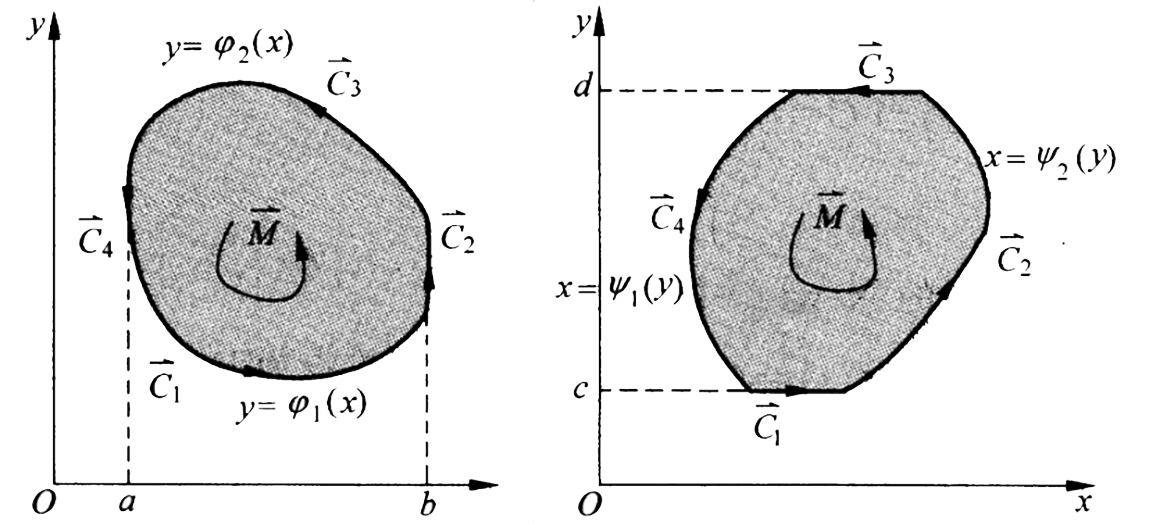
\includegraphics[width=0.8\textwidth]{img/SpecialRegion1.png}
    \caption{Two special orientated closed regions.}
    \label{fig:SpecialRegion1}
\end{figure}

Denote \(\oint_{\overset{\rightharpoonup}{\partial M}}\) as the line integral 
along the boundary of region \(\overset{\rightharpoonup}{M}\), then we have the following lemma.
\begin{lemma}
    \begin{enumerate}
        \item Let \(\overset{\rightharpoonup}{\partial M}\) be the first region in Fig~\ref{fig:SpecialRegion1},
            \(P(x, y) \in C^{1}(M)\), then:
            \[
            \oint_{\overset{\rightharpoonup}{\partial M}} P \, \mathrm{d}x = -\iint_{\overset{\rightharpoonup}{M}} \frac{\partial P}{\partial y} \, \mathrm{d}x \wedge \mathrm{d}y,
            \] 
        \item Let \(\overset{\rightharpoonup}{\partial M}\) be the second region in Fig~\ref{fig:SpecialRegion1},
            \(Q(x, y) \in C^{1}(M)\), then:
            \[
            \oint_{\overset{\rightharpoonup}{\partial M}} Q \, \mathrm{d}y = \iint_{\overset{\rightharpoonup}{M}} \frac{\partial Q}{\partial x} \, \mathrm{d}x \wedge \mathrm{d}y.
            \]
    \end{enumerate}
\end{lemma}

\begin{theorem}{Green's Theorem}
    Let \(\overset{\rightharpoonup}{M}\) be an orientated closed region in \(\mathbb{R}^{2}\),
    and \(\omega = P\mathrm{d}x + Q \mathrm{d}y \in C^{1}(M)\).
    If \(\overset{\rightharpoonup}{\partial M}\) can not only be split into finitely many first regions in Fig~\ref{fig:SpecialRegion1}
    (non-overlapping, no shared interior points),
    but also into finitely many second regions in Fig~\ref{fig:SpecialRegion1} (non-overlapping, no shared interior points),
    then:
    \[
    \oint_{\overset{\rightharpoonup}{\partial M}} P \, \mathrm{d}x + Q \, \mathrm{d}y = 
    \iint_{\overset{\rightharpoonup}{M}} \left( \frac{\partial Q}{\partial x} - 
    \frac{\partial P}{\partial y} \right) \, \mathrm{d}x \wedge \mathrm{d}y,
    \]
    or equivalently,
    \[
    \oint_{\overset{\rightharpoonup}{\partial M}} \omega = \iint_{\overset{\rightharpoonup}{M}} \mathrm{d}\omega,
    \]
    where \(\overset{\rightharpoonup}{\partial M}\) is the induced orientation of \(\overset{\rightharpoonup}{M}\).
\end{theorem}


\begin{leftbarTitle}{Gauß's Formula}\end{leftbarTitle}
Consider three kinds of special orientated closed surfaces in \(\mathbb{R}^{3}\) as shown in Figure \ref{fig:SpecialRegion2}.
As for the first surface \(\overset{\rightharpoonup}{M}\)
($\overset{\rightharpoonup}{M}$ adopts a positive orientation (right-hand system), 
and $\overset{\rightharpoonup}{\partial M}$ adopts the outward normal orientation), 
it consists of three orientated surfaces:
\begin{description}
    \item[\(\overset{\rightharpoonup}{\Sigma_1}\)] \(z = \varphi_{1}(x, y), (x, y) \in \Delta_{1}\),
    \item[\(\overset{\rightharpoonup}{\Sigma_2}\)] \(z = \varphi_{2}(x, y), (x, y) \in \Delta_{1}\),
    \item[\(\overset{\rightharpoonup}{\Sigma_3}\)] A cylindrical taking \(\partial \Delta_1\) as the directrix,
        with the generatrix paralleling to the \(Oz\)-axis. 
        Of course, it can also be reduced as a closed curve.
\end{description}
The second and third surfaces are similar.
\begin{figure}[h]
    \centering
    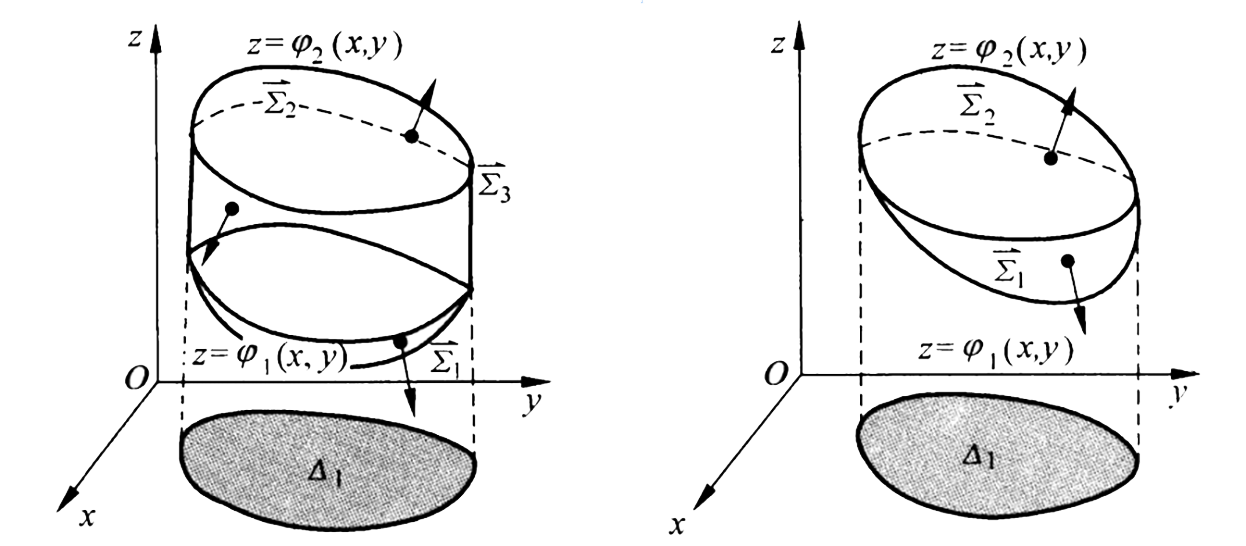
\includegraphics[width=0.8\textwidth]{img/SpecialRegion2.png}
    \caption{Three special orientated closed surfaces (only the first two are shown).}
    \label{fig:SpecialRegion2}
\end{figure}

Denote \(\oiint_{\overset{\rightharpoonup}{\partial M}}\) as the surface integral
over the boundary of region \(\overset{\rightharpoonup}{M}\), then we have the following lemma.
\begin{lemma}
    \begin{enumerate}
        \item Let \(\overset{\rightharpoonup}{\partial M}\) be the first surface in Fig~\ref{fig:SpecialRegion2},
            \(R(x, y, z) \in C^{1}(M)\), then:
            \[
            \oiint_{\overset{\rightharpoonup}{\partial M}} R \, \mathrm{d}x \wedge \mathrm{d}y = 
            \iiint_{\overset{\rightharpoonup}{M}} \frac{\partial R}{\partial z} \, \mathrm{d}x \wedge \mathrm{d}y \wedge \mathrm{d}z,
            \] 
        \item Let \(\overset{\rightharpoonup}{\partial M}\) be the second surface in Fig~\ref{fig:SpecialRegion2},
            \(P(x, y, z) \in C^{1}(M)\), then:
            \[
            \oiint_{\overset{\rightharpoonup}{\partial M}} P \, \mathrm{d}y \wedge \mathrm{d}z = 
            \iiint_{\overset{\rightharpoonup}{M}} \frac{\partial P}{\partial x} \, \mathrm{d}x \wedge \mathrm{d}y \wedge \mathrm{d}z,
            \]
        \item Let \(\overset{\rightharpoonup}{\partial M}\) be the third surface in Fig~\ref{fig:SpecialRegion2},
            \(Q(x, y, z) \in C^{1}(M)\), then:
            \[
            \oiint_{\overset{\rightharpoonup}{\partial M}} Q \, \mathrm{d}z \wedge \mathrm{d}x = 
            \iiint_{\overset{\rightharpoonup}{M}} \frac{\partial Q}{\partial y} \, \mathrm{d}x \wedge \mathrm{d}y \wedge \mathrm{d}z.
            \]
    \end{enumerate}
\end{lemma}

\begin{theorem}{Gauß's Theorem}
    Let \(\overset{\rightharpoonup}{M}\) be an orientated closed region in \(\mathbb{R}^{3}\),
    and \(\omega = P\mathrm{d}y \wedge \mathrm{d}z + Q \mathrm{d}z \wedge \mathrm{d}x 
    + R \mathrm{d}x \wedge \mathrm{d}y \in C^{1}(M)\).
    If \(\overset{\rightharpoonup}{\partial M}\) can not only be split into finitely many first surfaces 
    in Fig~\ref{fig:SpecialRegion2}
    (non-overlapping, no shared interior points),
    but also into finitely many second surfaces in Fig~\ref{fig:SpecialRegion2} (non-overlapping, no shared interior points),
    and into finitely many third surfaces in Fig~\ref{fig:SpecialRegion2} (non-overlapping, no shared interior points),
    then:
    \[
    \oiint_{\overset{\rightharpoonup}{\partial M}} P \, \mathrm{d}y \wedge \mathrm{d}z + Q \, \mathrm{d}z \wedge \mathrm{d}x + R \, \mathrm{d}x \wedge \mathrm{d}y = 
    \iiint_{\overset{\rightharpoonup}{M}} \left( 
        \frac{\partial P}{\partial x} + 
        \frac{\partial Q}{\partial y} + 
        \frac{\partial R}{\partial z} 
    \right) \, \mathrm{d}x \wedge \mathrm{d}y \wedge \mathrm{d}z,
    \]
    or equivalently,
    \[
    \oiint_{\overset{\rightharpoonup}{\partial M}} \omega = 
    \iiint_{\overset{\rightharpoonup}{M}} \mathrm{d}\omega,
    \]
    where \(\overset{\rightharpoonup}{\partial M}\) is the induced orientation of \(\overset{\rightharpoonup}{M}\).
\end{theorem}


\begin{leftbarTitle}{Stokes' Formula}\end{leftbarTitle}
\begin{theorem}{Stokes' Theorem}
    Let \(\overset{\rightharpoonup}{M}\) be an orientated smooth surface in \(\mathbb{R}^{3}\)
    with boundary \(\overset{\rightharpoonup}{\partial M}\),
    and \(\omega = P\mathrm{d}x + Q \mathrm{d}y + R \mathrm{d}z \in C^{1}(\Sigma)\).
    Then:
    \begin{align*}
        &\oint_{\overset{\rightharpoonup}{\partial M}} P \, \mathrm{d}x + Q \, \mathrm{d}y + R \, \mathrm{d}z\\
        =& \iint_{\overset{\rightharpoonup}{M}} \left( 
            \frac{\partial R}{\partial y} - \frac{\partial Q}{\partial z}
        \right) \, \mathrm{d}y \wedge \mathrm{d}z +
        \left( 
            \frac{\partial P}{\partial z} - \frac{\partial R}{\partial x}
        \right) \, \mathrm{d}z \wedge \mathrm{d}x +
        \left(
            \frac{\partial Q}{\partial x} - \frac{\partial P}{\partial y}
        \right) \, \mathrm{d}x \wedge \mathrm{d}y \\
        =& \iint_{\overset{\rightharpoonup}{M}} 
            \begin{vmatrix}\mathrm{d}y \wedge \mathrm{d}z&\mathrm{d}z \wedge \mathrm{d}x& \mathrm{d}x \wedge \mathrm{d}y\\
            \frac{\partial }{\partial x}&\frac{\partial }{\partial y}&\frac{\partial }{\partial z}\\
            P&Q&R            
            \end{vmatrix}\\
        =&\iint_{\overset{\rightharpoonup}{M}} 
        \begin{vmatrix}\cos\alpha&\cos\beta&\cos\gamma \\
        \frac{\partial }{\partial x}&\frac{\partial }{\partial y}&\frac{\partial }{\partial z}\\
        P&Q&R
        \end{vmatrix} \mathrm{d}S,
    \end{align*}
    or equivalently,
    \[
    \oint_{\overset{\rightharpoonup}{\partial M}} \omega = \iint_{\overset{\rightharpoonup}{M}} \mathrm{d}\omega,
    \]
    where \(\overset{\rightharpoonup}{\partial M}\) is the induced orientation of \(\overset{\rightharpoonup}{M}\).
\end{theorem}

\section{Closed and Exact Differential Forms}
\begin{definition}{Closed and Exact Differential Forms}
    Let \(U \subset \mathbb{R}^{n}\) be an open set and \(\omega\) be a \(C^{r}(r\geqslant 1)\) \(k\)-form on \(U\).
    \begin{enumerate}
        \item If \(\mathrm{d}\omega = 0\), then \(\omega\) is called a \textbf{closed form}.
        \item If there exists a \(C^{r+1}\) \((k-1)\)-form \(\eta\) such that \(\omega = \mathrm{d}\eta\),
            then \(\omega\) is called an \textbf{exact differential form}.
    \end{enumerate}
\end{definition}



\section{Introduction to Field Theory}

\chapter{Improper Integrals with Variable Parameters}




\begin{thebibliography}{99} 
\bibitem{1} 徐森林, 薛春华. \emph{数学分析 (1st edition) }. 清华大学出版社, 2005.
\bibitem{2} 陈纪修, 於崇华. \emph{数学分析 (3rd edition) }. 高等教育出版社, 2019.
\bibitem{3} 常庚哲, 史济怀. \emph{数学分析教程 (3rd edition) }. 中国科学技术大学出版社, 2012.
\bibitem{4} 裴礼文. \emph{数学分析中的典型问题与方法 (3rd edition) }. 高等教育出版社, 2021.
\bibitem{5} 汪林. \emph{数学分析中的问题与反例 (1st edition) }. 高等教育出版社, 2015.
\bibitem{6} 谢惠民, 恽自求, 易法槐, 钱定边. \emph{数学分析习题课讲义 (2nd edition) }. 高等教育出版社, 2019.
\bibitem{7} Walter Rudin. \emph{Principles of Mathematical Analysis (3rd edition) }. McGraw-Hill, 1976.
\bibitem{8} 菲赫金哥尔茨. \emph{微积分学教程 (8th edition) }. 高等教育出版社, 2006.
\bibitem{9} Wikipedia. \url{https://en.wikipedia.org/wiki/}.
\end{thebibliography}

\end{document}